\documentclass[12pt, a4paper]{report} \usepackage[titletoc]{appendix}
%\linespread{1.5}
%\usepackage{lineno}
%\linenumbers
\usepackage{amsmath}
\usepackage{float}
\usepackage[utf8]{inputenc}
\usepackage[T1]{fontenc}
\usepackage{lmodern}
\usepackage{microtype} % optional, for aesthetics
\usepackage{tabularx} % nice to have
\usepackage{booktabs}
\usepackage{makecell}
\usepackage{cite}
\usepackage{multirow}
\usepackage{hhline}
\usepackage{parskip}
\usepackage{wrapfig}
\usepackage{lscape}
\usepackage{xcolor}
\usepackage{ragged2e}
\usepackage{enumitem}
\usepackage{graphicx}
\usepackage{booktabs}
\setlist[enumerate]{label*=\arabic*.}
\usepackage{makecell}
\usepackage{kantlipsum}
\usepackage{enumitem}
\usepackage{tabularx}
\usepackage{appendix}
\usepackage{multirow}
\usepackage{hhline}
\usepackage{array}
\usepackage{subcaption}
%\usepackage{caption}
\graphicspath{{images/}} 
\usepackage{geometry}
\geometry{a4paper,left=4cm,top=3cm,bottom=3cm,right=3cm}
\usepackage{multirow}
\usepackage{hyperref}
\hypersetup{colorlinks=true,allcolors=blue}
\usepackage{hypcap}
\usepackage{courier}
\usepackage[linesnumbered,ruled]{algorithm2e}
\usepackage{listings}
\lstset{
    basicstyle=\ttfamily,
    frame=none, 
    breaklines=true,
    numbers=left,
    xleftmargin=2.5em,
    framexleftmargin=0em,
    emphstyle=\textbf,
    float=t
}
\lstdefinestyle{ocl}{
    emph={
        context, inv
    }
}
\lstdefinestyle{cbp}{
    basicstyle=\ttfamily\scriptsize,
    emph={
        session, create, type,
        set, to, add, hire
    }
}
\lstdefinestyle{xmi}{
    basicstyle=\ttfamily\scriptsize,
    emph={
        Node, children
    }
}
\lstdefinestyle{xml}{
    basicstyle=\ttfamily\scriptsize,
    emph={
        register, create, add, to, resource, at,
        from, eattribute, remove, ereference,
        set, unset, session, Roy, Jen,
        Moss, Richmond
    }
}
\lstdefinestyle{java}{
    basicstyle=\ttfamily\scriptsize,
    emph={
        case, $unset$,
        instanceof, else, if, void,
        new, UnsetEAttributeEvent,
        UnsetEReferenceEvent,
        @override, public, class, extends
    }
}
\lstdefinestyle{eol}{
    basicstyle=\ttfamily\scriptsize,
    emph={
        var, new, for, in, create, set, with, type, at,
        unset, to, add, remove, delete, register, move,
        from, position, from, move-within, session, \.
    }
}

\hyphenation{op-tical net-works semi-conduc-tor Hybrid-Change-Event-Adapter Hybrid-XMI-Change-Event-Adapater
    Hybrid-Neo-EMF-Change-Event-Adapater change-events Change-Event-Adapter EContent-Adapter notify-Changed Hybrid-Resource Resource-Impl state-Based-Resource cbp-Output-Stream Output-Stream Hybrid-Change-Event-Adapater Output-Stream Hybrid-XMI-Resource-Impl Hybrid-Neo-EMF-Resource-Impl Persistence-Resource change events
}


\definecolor{gray1}{gray}{0.90}
\definecolor{gray2}{gray}{0.95}

%\renewcommand{\thelstlisting}{\arabic{lstlisting}}
\renewcommand{\labelitemi}{$\bullet$}
\newcommand{\AndA}{\textnormal{\textbf{and }}}
\newcommand{\Is}{\textnormal{\textbf{is }}}
\newcommand{\Not}{\textnormal{\textbf{not }}}
\newcommand{\In}{\textnormal{\textbf{in }}}
\newcommand{\Or}{\textnormal{\textbf{or }}}
\newcommand{\eqnum}{\refstepcounter{equation}\textup{\tagform@{\theequation}}}

\begin{document}

\begin{titlepage}
\begin{center}

\textbf{\large Change-Based Model Persistence}

\vfill
\begin{figure}[ht]
\centering
\includegraphics[width=0.5\linewidth]{uoy}
\label{fig:uoy}
\end{figure}
\vfill

Alfa Ryano Yohannis\\
ary506@york.ac.uk

\vspace{1cm}

Supervisors:\\
Dimitris Kolovos\\
Fiona Polack\\
Horacio Hoyos Rodriguez
\vspace{1cm}

Department of Computer Science\\
University of York\\
United Kingdom\\
\vspace{1cm}
\today

\vfill
A Thesis Submitted in Partial Fulfillment of the Requirements\\
for the Degree of Doctor of Philosophy in Computer Science


\end{center}
\end{titlepage}


\begin{abstract}
\label{abstract}
\addcontentsline{toc}{chapter}{Abstract}
Most of the models in Model-Driven Engineering are persisted in state-based formats. While state-based persistence has certain advantages, it is problematic when it comes to detecting changes in large-scale models. As an alternative, this work proposes a change-based approach that involves persisting the full sequence of changes made to models. Persisting a model in a change-based format has the potential to deliver benefits over state-based persistence, such as the ability to detect changes, compare and merge models much faster and more precisely, which can then yield positive knock-on effects on helping developers compare and merge models in collaborative modelling environments. Nevertheless, change-based persistence also comes with downsides, such as ever-growing model file sizes and increased model loading time. So far, the initial implementation has been presented at the FlexMDE 2017 workshop, the proposed algorithm to optimise the loading time of change-based persistence has been presented at the ECMFA 2018 conference, and a paper discussing hybrid model persistence also has been presented at the Models and Evolution 2018 workshop. Currently, this research is still working on the change-based model comparison and merging. The thesis writing up is planned to start next year. An adjustment of the previous research plan is also presented in this report.
\end{abstract}

\tableofcontents
\addcontentsline{toc}{chapter}{Contents}

\cleardoublepage
\listoffigures
\addcontentsline{toc}{chapter}{List of Figures}

\cleardoublepage
\listoftables
\addcontentsline{toc}{chapter}{List of Tables}

\cleardoublepage
\lstlistoflistings
\addcontentsline{toc}{chapter}{Listings}

\cleardoublepage
\chapter*{Preface}

\cleardoublepage
\chapter*{Acknowledgements}
This work was partly supported through a scholarship managed by 
\emph{Lembaga Pengelola Dana Pendidikan Indonesia}
(Indonesia Endowment Fund for Education).

\cleardoublepage
\chapter*{Declaration}
I declare that this thesis is a presentation of original work and 
I am the sole author. This work has not previously been presented 
for an award at this, or any other, University. All sources are 
acknowledged as References.

\cleardoublepage
\chapter{Introduction}
\label{ch:introduction}
This Chapter briefly presents the background of this work as well as the research questions that will be 
addressed in this project. Several research objectives are then defined to answer the research questions. 
Lastly, research outputs and scoping are also presented. 

\section{Background}
\label{sec:background}
Most of the models in the context of Model-Driven Engineering are persisted in state-based formats. 
In such approaches, model files contain snapshots of the models' contents, and activities like version control 
and change detection are left to external systems such as file-based version-control systems and model differencing 
facilities. Activities such as change-detection (identifying parts that have changed in a model compared 
to a previous version) and model comparison (finding differences between models) are computationally consuming
for state-based models \cite{Kolovos:2009:DMM:1564596.1564641}. Thus, a new approach is needed to make the 
computation more efficient.

As an alternative to state-based persistence, this work proposes that a model can also be persisted in a change-based format, 
which persists the full sequence of \emph{changes} made to the model instead. 
The concept of change-based persistence is not new and has been used in persisting changes to software, 
object-oriented databases, and hierarchical documents 
\cite{DBLP:journals/entcs/RobbesL07,DBLP:conf/sde/LippeO92,DBLP:conf/caise/IgnatN05}. 
The change-based approach can improve detecting differences more precisely at the semantic 
level -- that is by providing finer-granularity information (e.g. types of changes, the order of the changes, 
elements that were changed, previous values, etc.) -- and therefore provide support to resolve them \cite{mens2002state}. 
The ordered nature of change-based persistence means that changes made to a model can be identified sequentially without 
having to explore and compare all elements of the model and its previous version. Based on these arguments, 
this work explores the advantages and shortcomings of change-based persistence as an alternative approach to 
state-based persistence for models conforming to 3-layer metamodelling architectures such as EMF and MOF. 
Persisting models in a change-based format can bring a number of envisioned benefits over state-based persistence, 
such as the ability to detect changes much faster and more precisely, which can then have positive 
knock-on effects on supporting (1) developers compare and merge models in collaborative modelling environments, 
and (2) incremental model management (e.g., incremental query \cite{DBLP:conf/ecmdafa/RathHV12} and 
model-to-text transformation \cite{DBLP:conf/ecmdafa/OgunyomiRK15}). 

Nevertheless, change-based persistence also comes with downsides, such as ever-growing model files 
\cite{DBLP:journals/entcs/RobbesL07,DBLP:conf/edoc/KoegelHLHD10} and increased model loading time \cite{mens2002state}
which increase storage and computation costs. A model that is frequently modified will increase considerably in file size 
since every change is added to the file. The increased file size (proportional to the number of persisted changes) will, 
in turn, increase the loading time of the model since all changes have to be replayed to reconstruct the model's 
eventual state. These downsides have to be mitigated to enable the practical adoption of change-based persistence. 
One approach to reducing the file size of change-based models is by removing changes that do not affect the eventual 
state of the model. For the increased loading time, it can be mitigated by ignoring -- i.e. not replaying -- changes 
that are cancelled out by later changes or employing change-based and state-based persistence side-by-side so that the
benefits of state-based persistence on loading time can be obtained. Other downsides are change-based persistence requires 
integration with existing tools -- since it is still a non-standard approach -- for its adoption \cite{koegel2010emfstore}, 
and still has limited support for standard, text-based version controls for collaborative development \cite{koegel2010emfstore}. 
These downsides can be addressed by developing a change-based persistence plugin for a specific development environment 
(e.g. Eclipse) and persisting changes in text-based format to support text-based version controls (e.g. Git, SVN).

\section{Research Questions}
\label{sec:research_questions}
The hypothesis of this work is that \textbf{``Change-based model persistence reduces the execution time of model differencing and conflict detection of large models compared to their execution time in state-based model persistence, with acceptable trade-offs on loading and persisting time, memory footprint, and storage space consumption''}. The execution time is the time required to complete the processes (e.g. change-detection, model comparison, model merging, or persisting changes). Model differencing is identifying the differences between two  versions of a model, which elements of features of the model that have different states. Model conflict detection is identifying changes applied to two versions of a model that cause an element or feature of the model has different states in both versions. This condition requires user decision to choose one of the possible states as the end state when both versions are merged.  This work refers ``large models'' to models with more than 1M elements, consistently with \cite{daniel2016neoemf,DBLP:conf/models/Espinazo-PaganCM11}. Model load time is the amount of time required to load a model from its persistence into memory. Persisting changes is saving changes made to a model into a persistent representation (e.g. a file). Memory footprint is the size of the memory occupied  at the time a process finished. Disk space consumption is the amount of storage consumed by the persistence. The term ``acceptable'' means that (1) the solutions proposed in this work deliver improvement on faster loading and saving time with less memory footprint compared to existing solutions as the baselines, or (2) the performance could be slightly worse but in rare condition or not statistically significant, or (3) the cost to accommodate the trade-off is affordable in the current context, such as the cost for extending memory and storage space.

To assess the validity of the hypothesis, this work aims to answer the following research questions: 
\begin{enumerate} 
\item \textbf{How to persist models in a change-based format? How does it perform compared to state-based persistence on loading and saving models? (RQ1)} 

The concept of change-based persistence has to be translated into an implementation in a modelling framework context so that it can be applied for model persistence, and therefore its impact on model loading and saving, model differencing, and model conflict detection can be assessed.

\item \textbf{How to identify differences between two versions of a change-based model? To what extent does change-based model differencing perform, in terms of speed and memory footprint, compared to state-based model differencing? (RQ2)} 

The purpose of using change-based persistence in this work is to speed up model differencing. Due to the nature of change-based persistence, the mechanism to perform change-based model differencing will differ substantially from the current state-based model differencing. It is expected that model differencing in change-based persistence perform faster than model differencing in state-based persistence.        

\item \textbf{How to detect conflicts between two versions of a change-based model? To what extent does change-based model conflict detection perform, in terms of speed and memory, compared to state-based model conflict detection? (RQ3)} 

The knock-on effect of change-based persistence on model conflict detection will also be investigated. It is expected that comparison of change-based models will be significantly faster than the comparison of state-based models.

%\item \textbf{How to merge different change-based models that come from the same ancestor? How does the merging perform compared to model merging in state-based persistence?}
%
%Another knock-on effect of faster change-detection of change-based persistence is faster model merging. Similar to the change-based model comparison, the mechanism to merge change-based models will differ substantially from merging state-based models. It is expected that the change-based model merging will be much faster than state-based model merging.   

\end{enumerate}

\section{Research Objectives}
\label{sec:research_objectives}
This research aims to meet the following research objectives to answer the research questions.
\begin{enumerate}
\item Develop an implementation of change-based persistence so it can be applied to persist models in change-based format, and evaluate the correctness of change-based models that it produces and its performance on saving changes against state-based persistence. 
\item Develop a solution to perform change-based model differencing, and compare its execution time and memory footprint against state-based model differencing.
\item Develop a solution to perform change-based model conflict detection, and compare its execution time and memory footprint against state-based model conflict detection.
\end{enumerate}

\section{Research Outputs}
\label{sec:research_outputs}
By the end of this research, these following outputs will have been produced:
\begin{enumerate}
\item Prototypes for change-based persistence. 
\item Solutions -- including their implementation and evaluation -- for loading time reduction and saving, model differencing, and model conflict detection of change-based persistence.
\item Publications and a thesis documenting the outcomes of this research.
\end{enumerate}

\section{Research Scope}
\label{sec:research_scope}
The scope of this research will be restricted to models conforming to 3-level metamodelling architectures. The Eclipse Modelling Framework will be used, as a representative example of such architectures, for the implementation of all algorithms and prototypes.

\section{Thesis Structure}
\label{sec:Thesis Structure}
This section provides the overview of each chapter presented in this thesis.

\subsection{Chapter 1: Introduction}
\label{sec:chapter_1_introduction_plan}
This chapter is intended to present the motivation and purpose of this research. It comprises the background of the research as well as the research hypothesis, research questions, research objectives, research outputs, research scope, thesis structure, and published papers. 

\subsection{Chapter 2: Literature Review}
\label{sec:chapter_2_literature_review_plan}
This chapter is dedicated to summarise work related to change-based persistence and comparison, critically assesses the advantages and disadvantages of current approaches, and seek the opportunities to contribute novel knowledge to the field. The chapter comprises brief discussion on methods to identify changes in models, the benefits of change-based solutions to model management, the advantages and drawbacks state and change-based persistence in the context of software engineering, the state of art of model persistence, the state of art of model comparison, state-based model differencing, state-based conflict detection, change-based conflict detection, and the research method applied in this work.

\subsection{Chapter 3: Change-based Model Persistence}
\label{sec:chapter_3_Change-based_model_ersistence_plan}
This chapter presents the concept of change-based model persistence and its core implementation. It comprises the concept of change-based model persistence, and the design of the core implementation. These contents have been published in a workshop \cite{DBLP:conf/models/YohannisKP17}.


\subsection{Chapter 4: Optimised Loading of Change-based Models}
\label{sec:chapter_4_optimised_loading_change_based_model_persistence}

Change-based persistence comes with a downside of ever-growing file sizes \cite{DBLP:journals/entcs/RobbesL07,DBLP:conf/edoc/KoegelHLHD10} which causes increased loading time \cite{mens2002state}. Reducing the loading time is essential to facilitate the practical adoption of change-based persistence. One way to reduce the increased loading time is by ignoring -- not replaying -- changes that are cancelled out by subsequent changes. 

To evaluate the efficiency of the proposed approach, the optimised loading is compared to a naive loading of a change-based representation and loading the same model from a state-based representation. They are compared on time required to load models and the memory footprint after loading models. Evaluation is also performed on time required for persisting changes between change-based and state-based persistence to show the benefit of change-based persistence on saving changes. 

This chapter is intended to present the optimisation approach along with its implementation and evaluation. The contents of this chapter is largely based on a published conference paper \cite{yohannis2018towards}. 

\subsection{Chapter 5: Hybrid Model Persistence}
\label{sec:chapter_5_hybrid_model_persistence}
While optimised loading is faster than the naive loading, the benefits are moderate and that the optimised loading is still slower than loading from a state-based representation \cite{DBLP:conf/models/YohannisRPK18}. This finding has motivated the design and development of a hybrid persistence approach, that is augmenting a change-based representation with a state-based representation. 

The hybrid model persistence approach is evaluated by comparing it to state-based persistence (e.g. XMI, NeoEMF \cite{daniel2016neoemf}) on time, memory footprint, and storage space required for loading models and persisting changes. The evaluation is also performed on time required for detecting changes between hybrid and state-based persistence to show the benefit of change-based persistence over state-based model comparison. 

This chapter is dedicated to present the hybrid model persistence approach together with its implementation and evaluation. The contents of this chapter is be largely based on a workshop paper \cite{DBLP:conf/models/YohannisRPK18}.

\subsection{Chapter 6: Efficient Model Differencing of Change-based Models}
\label{sec:chapter_6_model_differencing}
This chapter presents a change-based model differencing with its implementation and evaluation. Change-based persistence is expected to speed-up model differencing because the information required to identify changes is already contained in the models' persistence. 

The proposed model differencing is evaluated by comparing it to state-based model differencing on the time and memory footprint required to find all differences between two versions of a model. The contents of this chapter is be largely based on a workshop paper \cite{yohannis2018efficient}.

\subsection{Chapter 7: Efficient Conflict Detection of Change-based Models}
\label{sec:chapter_7_conflict_detection}
This chapter is planned to present change-based model conflict detection. After identifying the differences between two versions of a change-based model, this work also aims to detect conflict between two versions of a model. Model conflict detection is a crucial step that precedes model merging.

Similar to change-based model comparison in Section \ref{sec:chapter_6_model_differencing}, the proposed conflict detection is also evaluated by comparing it to the conflict detection of existing change and state-based persistence on the affected time and memory footprint.

\subsection{Chapter 8: Conclusions and Future Work}
\label{sec:chapter_8_conclusions_and_future_work}
This chapter summarises the work that has been carried and the evaluation results obtained in order to answer the research requestions and hypothesis proposed in Section \ref{sec:research_questions}. However, the conclusions also come with limitations and threat to validity which are also presented in the chapter. The chapter also presents the future work that can be done to address the limitations of this work, to extend the features of the proposed change-based model persistence, or for other research topics.

\section{Publications}
\label{sec:publications}
This research has published several papers in workshops and conferences. They are as follow:
\begin{enumerate}
  \item A. Yohannis, D. S. Kolovos, and F. Polack, ``Turning models inside out,'' in Proceedings of MODELS 2017 Satellite Events co-located with ACM/IEEE 20th International Conference on Model Driven Engineering Languages and Systems (MODELS 2017), Austin, TX, USA, September, 17, 2017., 2017, pp. 430–434. [Online]. Available: \url{http://ceur-ws.org/Vol-2019/flexmde_8.pdf}.
  \item  A. Yohannis, H. H. Rodriguez, F. Polack, and D. S. Kolovos, ``Towards efficient loading of change-based models,'' in Modelling Foundations and Applications - 14th European Conference, ECMFA 2018, Held as Part of STAF 2018, Toulouse,  France, June 26-28, 2018, Proceedings, 2018, pp. 235–250. [Online]. Available: \url{https://doi.org/10.1007/978-3-319-92997-2_15}.
  \item  A. Yohannis, H. H. Rodriguez, F. Polack, and D. S. Kolovos, ``Towards hybrid model persistence,'' in Proceedings of MODELS 2018 Workshops co-located with ACM/IEEE 21st International Conference on Model Driven Engineering Languages and Systems (MODELS 2018), Copenhagen, 
  Denmark, October, 14, 2018., 2018, pp. 594–603. [Online]. Available:  \url{http://ceur-ws.org/Vol-2245/me_paper_3.pdf}.
  \item  A. Yohannis, H. H. Rodriguez, F. Polack, and D. Kolovos,``Towards efficient comparison of change-based models,'' B. Combemale and A. Shaukat, Eds., vol. 18, no. 2, Jul. 2019, pp. 7:1–21, the 15th European Conference on Modelling Foundations and Applications. [Online]. Available: 
  \url{http://www.jot.fm/contents/issue_2019_02/article7.html}.
\end{enumerate}

\chapter{Literature Review}
\label{ch:literature_review}

This chapter presents the literature review of this study. Firstly, it discusses some work on model persistence by highlighting some key characteristics -- unique features, strong points, and downsides -- of some existing implementations. It then summarises the advantages and drawbacks of the two main types of persistence: state-based and change-based persistence, and introduces desirable characteristics for a new change-based persistence implementation. This chapter then reviews the related work on identifying differences and detecting conflicts between versions of models. It then presents the current challenges that model differencing and conflict detection are dealing with as well as the downsides of existing approaches in tackling the problems, which gives motivation to this research to come up with a new solution. Lastly, the conclusions of the literature review are presented.  

%\section{Introduction}
%\label{sec:introduction_2}
%The research introduced in this thesis aims at enabling high-performance model differencing and conflict detection through change-based persistence. This goal can only be delivered if this study can identify the strong points and downsides of current approaches of model persistence, differencing, and conflict detection and incorporate and address them in the solution of this research. Knowing the strong points and downsides is also helpful to find rooms for improvement and to deliver novelties in the solution. A literature review needs to be conducted in order to identify the strong points and downsides. The literature review of this study is presented in this chapter.
%
%Once the strong points, downsides, rooms for improvements and novelties have been gathered, they all need to be elaborated into a design of a solution. The solution needs to be translated into a working implementation, experimented, and evaluated to answer the research questions of this study. This sequence of work has to be guided by a research method to ensure it has been carried out properly. The research method employed in this study is also presented in this chapter. 
%
%The rest of this chapter is structured as follows. Section \ref{sec:model_persistence} reviews some key implementations of model persistence; their strong points and drawbacks. Section \ref{sec:model_differencing_and_conflict_detection} presents the current approaches in model differencing and conflict detection, their existing challenges, as well as the motivation for a new change-based model persistence. Section \ref{sec:benefits_and_novel_capabilities} presents briefly the research method employed in this research. Section \ref{sec:conclusions_2} concludes this chapter.

\section{Models in This Research}
\label{sec:models_in_this_research)}

A model is an abstract representation of an entity \cite{volter2013model}. It can be used for different purposes: as a sketch to communicate a system, as a blueprint to define the specification of a system, or as a modifiable artefact to generate a working system \cite{fowler2019umlmode}. In model-based software engineering, the latter is the case in which models are mainly used. 
In this context, a model are created using a modelling language, and the model should conform to its metamodel -- an abstraction that describes the model. Later, the model can be transformed to generate a software artefact through model transformation/code generation \cite{brambilla2012model}. The software artefact, its model, and the model's metamodel of its model create three layers of abstraction which are known as the 3-layer metamodelling architecture.  

Eclipse Modeling Framework (EMF) \cite{steinberg2008emf} is a technical implementation of such architecture. It is a framework and code generation facility that allows developers to define metamodels, create models, and to generate implementations of the models \cite{steinberg2008emf}. In this literature review, we focus on modelling tools that support the 3-layer metamodelling architecture of EMF.

\section{Model Persistence}
\label{sec:model_persistence}
In constructing models, modelling tools should be able to support model persistence so that models that are under construction can be saved at any time and reloaded for further modification. Majority of the tools persist models in a state-based format that is capturing a snapshot of a model at a time and then persist its entire state into storage. The model state can be persisted in different forms, such as text files, relational databases, or NoSQL databases.

\subsection{Text Files}
\label{sec:text_file}
The simplest and most common way to save a model is to persist it into a text file. By default, modelling tools that support the 3-layer metamodelling architectures of Eclipse Modeling Framework (EMF) \cite{steinberg2008emf} persist a model in a text file with a format of Metadata Interchange (XMI) -- a standard issued by Object Management Group (OMG) for exchanging metadata information via Extensible Markup Language (XML) \cite{omg2018xmi}. 

Since it is the default standard for persisting EMF models, it is supported by  most modelling tools. In order to modify a model persisted in an XMI file, such as performing create, read, update, delete (CRUD) operations, a tool has to de-serialise and load the model from the file into memory. This can be a problem when we only want to make a small number of changes but the size of the model is very large -- it takes considerable time and memory to load the model. Also, when saving, the model has to be persisted in its entirety causing inefficiency when we only made small number of changes. Since it is a text-based file, the model can be duplicated and shared with minimum effort, e.g. through manual copy or version control systems (e.g. Git \cite{git2019about}, SVN \cite{apache2019svn}). However, for model differencing (see Section \ref{sec:model_differencing_and_conflict_detection}), text-based differencing \cite{DBLP:journals/algorithmica/Meyers86} cannot be applied accurately to XMI files since essentially they are tree documents which require different differencing approaches \cite{wang2003xdiff}.

\subsection{Relational Databases}
\label{sec:relational_databases}
Models can also be persisted into relational databases. EMF Teneo \cite{eclipse2017teneo} is a solution that integerates EMF with existing persistency solutions, such as Hiberbate \cite{hibernate2019hibernateorm} and EclipseLink \cite{eclipse2019eclipselink}. Thus it can persists EMF models into relational database backends. In this way, EMF Teneo can utilise the power of storage, caching, and querying of the database backends. It also supports the automatic mapping of models to relational model schema with flexible mapping customisation. Using relational databases as its backends enables EMF Teneo to support lazy loading of models. So, when performing CRUD operations, it only loads and saves relevant elements and features -- not the entire model -- into and from memory, which is efficient in terms of memory usage.

Similar to EMF Teneo, Connected Data Objects (CDO) \cite{eclipse2019cdo} also supports persisting models into various database-backends model persistence (e.g. relational and NoSQL databases). It is a development-time model and metamodel repository as well as a distribution and runtime persistence framework for EMF-based application systems. It supports model versioning and can perform model differencing and conflict detection -- it uses EMF Compare \cite{emfcompare2018developer} to perform the comparison \cite{cdo2019emfcompare}. One downside of CDO is its adoption necessitates the use of a separate version control system (e.g. a Git repository for code and a CDO repository for models), which introduces fragmentation and administration challenges \cite{barmpis2014evaluation}.

\subsection{NoSQL Databases}
\label{sec:NoSQL Databases}
In the era where data is abundant and models are getting larger in sizes, the ability to handle large models is necessary. Tools, such as Morsa \cite{DBLP:conf/models/Espinazo-PaganCM11} and NeoEMF \cite{daniel2016neoemf}, has been developed to persist models into non-relational (NoSQL) databases. Morsa saves models in documents with MongoDB as its backend \cite{mongodb}, while NeoEMF persists models in multi, NoSQL backends: Neo4j \cite{neo4j2019neo4j} for Graph, MapDB \cite{mapdb2019mapdb} for Map, and Apache HBase \cite{apache2019hbase} for Column datastores. The advantages of using NoSQL databases are that users are given options to choose which datastores -- wih some degree for configuration -- that best fit with the characteristics of their models and metamodels and to maximise the features  the backends provide, such as lazy loading, caching, etc. Neither Morsa nor NeoEMF provide built-in support for versioning and models are eventually stored in binary files/folders which are known to be a poor fit for text-oriented version control systems like Git and SVN. 

\subsection{Change-based Representation}
\label{sec:change_based_representation}
All the solutions previously mentioned persist models in state-based format. EMF Store \cite{koegel2010emfstore} takes a different approach; it persists models in a change-based representation. EMF Store appears to be the only current implementation of change-based persistence for EMF models.

EMF Store is a model repository and supports collaborative editing and versioning of models \cite{emfstore2019what}. Instead of using standard text-oriented version controls (e.g., Git, SVN) for model versioning, EMF Store has its own dedicated, change-based, model-oriented versioning mechanism. Models are shared through a server and distributed to client applications. Clients can modify the models in parallel, offline or online, and synchronize with the server. Conflicts caused by concurrent modification are detected automatically and can be resolved interactively by users. The historical changes of models are kept on the server, and different versions of a model as well as changes that produce the them can be retrieved from the server. 

In EMF Store, to version models, a project has to be created first. A project can contain one or more models. Every project has a version history, and each version represents a commit of a client. A commit sends a package of changes to the server. The package itself contains a collection of operations applied to a version that transforms it to a newer version or can be said as the deltas between the two versions. The operations can be add, delete, set, unset or move that modifies an element or feature, or they can be a composite operation, an operation that consists of many operations, e.g. refactoring that moves a method to a superclass.

To obtain a specific version of an existing project, a client can perform a checkout. This version is called the base version on the client side. The client then can perform modification to this version. Every operation applied to the version is recorded by EMF Store. When the client commits, these operations are put into one package and sent to the server. If the base version is still the head version of the project on the server, the commit is accepted, and a new version is created. If they are different, it means that there is another client that already committed its changes to the server. Thus the current client has to synchronise it by updating its local project. This is the state where conflicts can happen potentially between the incoming and local changes, that is when they modify the same element or feature of a model. EMF Store performs conflict detection to identify conflicts automatically. The mechanism of EMF Store to identify conflicts is discussed in detail in Section \ref{sec:emfstore_conflict_detection}.

\begin{table*}[]
  \centering
  \caption{Advantages and downsides of different model persistence solutions.}
  \label{table:model_persistence_comparison}
\begin{scriptsize}
  \begin{tabular}{
      |>{\centering\arraybackslash}m{0.1\linewidth}
      |>{\centering\arraybackslash}m{0.4\linewidth}
      |>{\centering\arraybackslash}m{0.4\linewidth}
      |}
    \hline
    \textbf{Products} & \textbf{Advantages} & \textbf{Downsides} \\
    \hline
    XMI 
    &
    \begin{minipage}[t]{\linewidth}
      \raggedright
      \begin{itemize}[leftmargin=7pt]
        \setlength
        \item[+] default standard, widely supported
        \item[+] easy to be duplicated and shared by manual copy or text-oriented version controls
      \end{itemize}
    \end{minipage}
    & 
    \begin{minipage}[t]{\linewidth}
      \raggedright
      \begin{itemize}[leftmargin=5pt]
        \setlength
        \item[--] requires loading the entire model to modify
        \item[--] a model is saved in its entirety
        \item[--] supports text-oriented version controls, but applying text-based differencing might produce inaccurate results    
      \end{itemize}
    \end{minipage}
    \\
    \hline
    Teneo 
    & 
    \begin{minipage}[t]{\linewidth}
      \raggedright
      \begin{itemize}[leftmargin=7pt]
        \setlength
        \item[+] supports lazy loading, only load and save affected elements and features when performing CRUD operations
        \item[+] has the capabilities supported by database backends: rollback, caching, etc. 
      \end{itemize}
    \end{minipage}
    &
    \begin{minipage}[t]{\linewidth}
      \raggedright
      \begin{itemize}[leftmargin=7pt]
        \setlength
        \item[--] does not support model versioning, comparison, and merging
        \item[--] multiple concurrent accesses can cause a bottleneck
%        \item[--] performance on loading and saving for CRUD operations depends on the database backend
        \item[--] poor fit for text-oriented version controls since models are persisted in database
      \end{itemize}
    \end{minipage} 
    \\
    \hline
    CDO
    &
    \begin{minipage}[t]{\linewidth}
      \raggedright
      \begin{itemize}[leftmargin=7pt]
        \setlength
        \item[+] supports lazy loading, only load and save affected elements and features when performing CRUD operations
        \item[+] supports model versioning, comparison, and merging
        \item[+] has the capabilities supported by database backends: rollback, caching, etc. 
      \end{itemize}
    \end{minipage}
    &
    \begin{minipage}[t]{\linewidth}
      \raggedright
      \begin{itemize}[leftmargin=7pt]
        \setlength
%        \item[--] performance on loading and saving for CRUD operations depends on the database backends
        \item[--] fragmentation and administration challenges due to separation of version controls between models and code
        \item[--] poor fit for text-oriented version controls since models are persisted in database
      \end{itemize}
    \end{minipage} 
    \\
    \hline
    Morsa \& NeoEMF 
    & 
    \begin{minipage}[t]{\linewidth}
      \raggedright
      \begin{itemize}[leftmargin=7pt]
        \setlength
        \item[+] supports lazy loading, only load and save affected elements and features when performing CRUD operations
        \item[+] has the capabilities supported by NoSQL backends: handling big data, graph data, etc.
      \end{itemize}
    \end{minipage}
    &
    \begin{minipage}[t]{\linewidth}
      \raggedright
      \begin{itemize}[leftmargin=7pt]
        \setlength
        \item[--] does not support model versioning, comparison, and merging
%        \item[--] performance on loading and saving for CRUD operations depends on the database backends
        \item[--] poor fit for text-oriented version controls since models are persisted in database
      \end{itemize}
    \end{minipage} 
    \\
    \hline
    EMF Store
    &
    \begin{minipage}[t]{\linewidth}
      \raggedright
      \begin{itemize}[leftmargin=7pt]
        \setlength
        \item[+] supports semantic versioning of models that allows model merging and conflict detection to be more effective
      \end{itemize}
    \end{minipage}
    &
    \begin{minipage}[t]{\linewidth}
      \raggedright
      \begin{itemize}[leftmargin=7pt]
        \setlength
        \item[--] requires loading the entire model to modify
        \item[--] a model is saved in its entirety even for small changes
        \item[--] persists models in the forms of files/folders and using its own mechanism for model versioning thus poor fit for text-oriented version controls
      \end{itemize}
    \end{minipage} 
    \\
    \hline
  \end{tabular}
\end{scriptsize}
\end{table*}
  
The primary motivation EMF Store applies change-based approach is that calculating the differences between two versions in state-based persistence can be expensive and less accurate \cite{emfstore2019versioning} (state-based model differencing identify differences using LCS algorithms \cite{emfcompare2018developer,DBLP:journals/algorithmica/Meyers86}, not from the real changes). Since it follows a change-based approach, it does not store the state of every version. It only saves operations of each version in an ordered manner so that they can be executed and reversed to obtain the states between versions. Nevertheless, it also stores the intermediate cached states for selected versions, including the head version, to speed up the retrieval of specific versions.

The advantages of EMF Store are that it was designed to allow semantic versioning of models, which can support model differencing and conflict detection to be more accurate and efficient rather than performing them on state-based model persistence \cite{emfstore2019versioning}. By default, the packages of operations are persisted in XMI files but it can also be configured to use other backends, e.g. MongoDB \cite{emfstore2019mongodb}. The downsides of EMF Store are it has its own mechanism for controlling versions thus limits its adopters to use common text-oriented version controls \cite{emfstore2019getting}, such as Git and SVN . Its performance can also degrade as more models/users are added to a repository \cite{KolovosRMPGCLRV13}.

The summary of the advantages and downsides of the different model persistence solutions presented in this section can be found in Table \ref{table:model_persistence_comparison}. These advantages and downsides give this research some points to consider on how a change-based model persistence format that is compatible with version control systems such as Git and SVN should be designed. These considerations are presented in Section \ref{sec:a_new_change_based_persistence}.

\subsection{Change-based vs. State-based Persistence}
\label{sec:change_based_vs_state_based_persistence}
This section compares the advantages and drawbacks of change-based and state-based persistence. Change-based persistence works by persisting the complete change history of an artefact instead of persisting a snapshot -- the entire state -- of an artefact at a time. The concept of change-based persistence is not new and has been used in persisting changes of software, object-oriented databases, hierarchical documents, and models 
\cite{DBLP:journals/entcs/RobbesL07,DBLP:conf/sde/LippeO92,DBLP:conf/caise/IgnatN05,koegel2010emfstore}. 

Change-based persstence offers two main advantages. First, it records finer-granularity information (e.g. types of changes, the order of the changes, elements that were changed, previous values, etc.) of changes which can improve the accuracy of change detection \cite{DBLP:journals/entcs/RobbesL07,DBLP:conf/sde/LippeO92,DBLP:conf/caise/IgnatN05,mens2002state}. Second, it records changes in an ordered manner which means that changes made to an artefact can be identified sequentially without having to explore and compare all elements of compared versions of an artefact \cite{DBLP:conf/edoc/KoegelHLHD10}. The advantages to detect changes more precisely and much faster can then have positive knock-on effects on supporting (1) developers compare and merge artefacts in collaborative environments \cite{DBLP:conf/sde/LippeO92,DBLP:conf/caise/IgnatN05,koegel2010emfstore}, and (2) incremental management \cite{jouault2010towards,DBLP:conf/ecmdafa/OgunyomiRK15, DBLP:conf/ecmdafa/RathHV12}. Moreover, changed-based persistence contains wealth information which can be exploited for analytics \cite{DBLP:journals/entcs/RobbesL07}.

Nevertheless, change-based persistence also comes with downsides, such as ever-growing artefact files  \cite{DBLP:journals/entcs/RobbesL07,DBLP:conf/edoc/KoegelHLHD10} and increased artefact loading time \cite{mens2002state} which increases storage and computation costs. An artefact that is frequently modified will increase considerably in file size since every change is added to the file. The increased file size (proportional to the number of persisted changes) will, in turn, increase the loading time of the artefact since all changes have to be replayed to reconstruct the artefact's eventual state. 

%These downsides have to be mitigated to enable the practical adoption of change-based persistence. 
%One approach to reducing the file size of change-based models is by removing changes that do not affect the eventual 
%state of the model. For the increased loading time, it can be mitigated by ignoring -- i.e. not replaying -- changes 
%that are cancelled out by later changes or employing change-based and state-based persistence side-by-side so that the
%benefits of state-based persistence on loading time can be obtained. 

Other downsides are change-based persistence requires 
integration with existing tools -- since it is still a non-standard approach -- for its adoption \cite{koegel2010emfstore}, 
and still has limited support for standard, text-based version controls for collaborative development \cite{koegel2010emfstore}. 
These downsides can be addressed by developing a change-based persistence plugin for a specific development environment 
(e.g. Eclipse) and persisting changes in text-based format to support text-based version controls (e.g. Git, SVN).

In summary, state-based persistence has several strong points. First, since it is the default standard persistence approach for most artefacts, it requires minimum effort to integrate with existing tools \cite{koegel2010emfstore}. Second, it is faster in loading artefacts persisted in state-based format since there is no need to replay all changes as in change-based persistence. Also, some of the artefacts support lazy loading. For example, an artefact is not loaded in entirety upfront. Only parts affected by an operation are loaded into memory. This enables faster CRUD (create, read, update, delete) operations \cite{DBLP:conf/models/Espinazo-PaganCM11,daniel2016neoemf}. 

\begin{table*}[h]
  \centering
  \caption{The advantages and downsides between change-based and state-based persistence.}
  \label{table:advantages_drawbacks}
\begin{scriptsize}
    \begin{tabular}
      {|>{\centering\arraybackslash}p{1.1cm}|>{\centering\arraybackslash}p{1.1cm}|>{\centering\arraybackslash}p{5cm}|>{\centering\arraybackslash}p{5cm}|}
      \hline 
      \multicolumn{2}{|c|}{\textbf{Dimensions}}&\textbf{Change-based Approach}&\textbf{State-based Approach}\\
      \hline 
      \multicolumn{2}{|p{2.2cm}|}{\centering Advantages} &
      \begin{minipage}[t]{5cm}
        \begin{itemize}[leftmargin=9pt]
          \setlength\itemsep{2pt}
          \item[+] Faster for detecting changes \cite{DBLP:conf/edoc/KoegelHLHD10}
          \item[+] More accurate, carry semantic information \cite{DBLP:journals/entcs/RobbesL07,DBLP:conf/sde/LippeO92,DBLP:conf/caise/IgnatN05,mens2002state}  
          \item[+] Faster and more accurate for comparison and merging \cite{DBLP:conf/sde/LippeO92,DBLP:conf/caise/IgnatN05,koegel2010emfstore}
          \item[+] Information carried is useful for analytics \cite{DBLP:journals/entcs/RobbesL07}
        \end{itemize}
      \end{minipage}
      & 
      \begin{minipage}[t]{5cm}
        \raggedright
        \begin{itemize}[leftmargin=9pt]
          \setlength\itemsep{2pt}
          \item[+] Faster for loading large artefacts \cite{DBLP:conf/models/Espinazo-PaganCM11,daniel2016neoemf,eclipse2019cdo}
          \item[+] A default standard, no need integration with existing tools \cite{koegel2010emfstore}  
        \end{itemize}
      \end{minipage}
      \\
      \hline
      \multicolumn{2}{|p{2.2cm}|}{\centering Disadvantages} & \begin{minipage}[t]{5cm}
        \raggedright
        \begin{itemize}[leftmargin=9pt]
          \setlength\itemsep{2pt}
          \item[--] Increased record size \cite{DBLP:journals/entcs/RobbesL07,DBLP:conf/edoc/KoegelHLHD10}
          \item[--] Is not efficient for replaying (loading) long records \cite{mens2002state}
          \item[--] Limited supports from standard, text-based version controls (e.g. GitHub) \cite{koegel2010emfstore} 
          \item[--] Not a standard, need integration with existing tools \cite{koegel2010emfstore} 
        \end{itemize}
      \end{minipage}
      & 
      \begin{minipage}[t]{5cm}
        \raggedright
        \begin{itemize}[leftmargin=9pt]
          \setlength\itemsep{2pt}
          \item[--] Slower for saving changes  \cite{mens2002state,daniel2016neoemf,DBLP:conf/models/Espinazo-PaganCM11}
          \item[--] Slower for comparison \cite{DBLP:conf/edoc/KoegelHLHD10}
          \item[--] Less accurate, does not carry semantic information \cite{mens2002state,DBLP:conf/edoc/KoegelHLHD10}  
        \end{itemize}
      \end{minipage}
      \\
      \hline
    \end{tabular} 
  \end{scriptsize}
\end{table*}

Compared to change-based persistence, state-based persistence also has  downsides. First, it is slower than change-based persistence in saving changes \cite{mens2002state}. For an artefact persisted in state-based format and does not support lazy loading, the the artefact has to be persisted in its entirety even thought only a single change has been made. Second, state-based persistence does not have any records of changes of an artefact. Thus, every part of the artefact has to be checked for differences which can be less efficient if the comparison is performed in change-based format \cite{DBLP:conf/edoc/KoegelHLHD10}. Third, since comparison in state-based format requires deriving differences through a diffing process -- not based on actual change records, it can be less accurate than comparison in change-based persistence which is provided with more information to detect changes accurately \cite{mens2002state,DBLP:conf/edoc/KoegelHLHD10}. The summary of the advantages and downsides between change-based and state-based persistence are presented in Table \ref{table:advantages_drawbacks}.

\section{Model Differencing and Conflict Detection}
\label{sec:model_differencing_and_conflict_detection}
The history of model differencing and conflict detection can be traced back to the presence of \textsf{diff} program on Unix or Unix-like platform \cite{hunt1976algorithm}. The program can perform diffing that is comparing text files ``in order to determine how or whether they differ'' \cite{diff}. Diffing basically is about finding the longest common subsequence between two or more sequences which commonly known as the Longest Common Subsequence (LCS) algorithms \cite{bergroth2000lcs}. This problem is equivalent to the Shortest Edit Script (SES) problem that is to find the smallest number of editing (add and delete) in order to make a sequence equal to another sequence \cite{DBLP:journals/algorithmica/Meyers86}. LCS or SES algorithms are commonly implemented by Version Control Systems, such as SVN \cite{svn-diff} and Git \cite{git-diff}, in their \textsf{diff} programs to identify differences between versions of files.   

Applying this diffing approach to some graph-based artefacts, such as XML \cite{w3c-xml} and Ecore models \cite{steinberg2008emf}, is not straightforward since they have different characteristics to text files. For example, XML is a hierarchical document with a tree structure; one node can contains other nodes. The unique feature of XML is that its containment is  unordered whereas in text differencing order is a necessary feature. This has been addressed by Wang et al. \cite{wang2003xdiff} by exploiting key XML  structure characteristics. Identifying differences between Ecore models is even more complex since the models support multiple characteristics of features, such as attribute/reference, literal/object values, single/multiple values, containment/non-containment, etc \cite{steinberg2008emf}. 

There are several existing tools for model differencing. 
EMF Compare \cite{emfcompare2018developer} is a popular tool used to compare and merge EMF models, with generic support for different metamodels. It is an extensible framework so that it can be adapated to the specific needs of certain metamodels. EMF Compare works by performing matching between elements of models being compared and then executing differencing to identify differences between the matched elements. Matching and differencing are discussed in detail in Chapter \ref{ch:model_differencing}. In this study, EMF Compare is used as a baseline for comparative evaluation due to its maturity and ongoing development activity. EMF DiffMerge (EDM) \cite{eclipse2019emfdiffmerge} is similar to EMF Compare except that its abstraction is at a lower level, and it is designed to prevent data loss and enforce model consistency \cite{eclipse2019emfdiffmerge2}. As a consequence, EMF Compare could use the EDM engine when it needs to enforce a particular consistency policy. Also, it supports scoping which means comparison does not have to be at the model level but could also be applied on arbitrarily-defined sets of model elements -- subsets of models -- that can be defined by specific filters \cite{jaxenter2019emfdiffmerge}. EMF Compare is used in this study used for comparative evaluation due to its maturity and ongoing development activity. Other tools, such as SiDiff \cite{Treude2007SiDiff} and DSMDiff \cite{lin2009dsmdiff},  also provide language-agnostic graph-based model comparison, with some room for configuration (e.g., assigning different weights to features of types in the language). Additional expressive power -- at the cost of increased complexity and configuration effort -- is offered by dedicated comparison languages such as the Epsilon Comparison Language, which can be used to compare both homogeneous and heterogeneous models \cite{kolovos2009ecl}. All of these tools work with state-based persistence to identify differences between models.

Our literature review has not revealed any other work that targets comparison of change-based models persisted in text files. Only EMF Store \cite{koegel2010emfstore} identified addresses change-based model conflict detection but it persists models in its own dedicated backend system. Moreover, since it is designed to identify conflicts between changes, it does not give direct, summarised information about which parts of two versions of a model are different -- not for model differencing. Database or dedicated-backend model persistence and version control solutions such as CDO \cite{eclipse2019cdo} and EMF Store provide model comparison capabilities between different versions of the same model but they present integration challenges when users wish to use text-oriented version control systems (e.g. Git, SVN) which are typically file-based and commonly used, and their performance can also degrade as more models/users are added to a repository \cite{KolovosRMPGCLRV13}.

\subsection{The Challenges of Model Comparison}
\label{sec:the_key_challenge_of_incrementality}

The performance of identifying differences between versions of models can become crucial for large evolving models, particularly in the latter phases of the development cycle when many small changes made to models to fine-tune them \cite{selic2003pragmatics}. This challenge has been addressed in incremental model management where changes of models are recorded and used as the basis to perform effective incremental model processing operations. In his work, Egyed \cite{egyed2011automatically} has shown that the property-access recording approach is applicable to query such changes. More recent work has shown that variants of this approach can be used to achieve incrementality in a wide range of model processing operations, including model-to-model transformation \cite{jouault2010towards}, model-to-text transformation \cite{DBLP:conf/ecmdafa/OgunyomiRK15}, model validation, and pattern matching \cite{DBLP:conf/ecmdafa/RathHV12}---as long as changes to models can be precisely identified.  

Nonetheless, this approach works best at identifying differences between serial versions of a model; it does not work straightforwardly to identify differences between parallel -- branched -- versions. In addition, the solutions in incremental model management are coupled to their execution engines, which limits itself to work best only in single-developer environment (discussed more in Section \ref{sec:identifying_changes_in models}). In a collaborative setting, as the sizes and complexity of models grows, it is common to manage a model in multiple parallel versions. Thus, capabilities to identify differences differencing between these parallel versions and to detect conflicts between the differences are also necessary.

Before merging two versions, model differencing and conflict detection need to be executed first in order to identify differences and conflicts between. Nevertheless, performing the model differencing and conflict detection in traditional, state-based way is computationally expensive and memory greedy (discussed more in Section \ref{sec:identifying_changes_in models}). Traditional, state-based model comparison requires every element of the versions being compared to be loaded into memory, matched, and then differenced \cite{emfcompare2018developer}, which is inefficient for large models that only undergo a small number of changes. A novel approach is required that can compare only elements that have been modified -- not all elements -- to speed up model comparison.

\subsection{Identifying Changes in Models}
\label{sec:identifying_changes_in models}
There are two approaches in the literature for identifying changes in models: using notification facilities and model differencing.

\subsubsection{Notifications}
\label{sec:notifications}
In this approach, a model change tracking 
engine needs to hook into the notification facilities 
provided by the modelling tool through which the developer edits the model, 
so that the engine can directly receive notifications as soon as 
changes happen (e.g. class \textsf{Giant} has been deleted, class \textsf{Character} has been renamed to ``Hero''). 
This is an approach taken by the IncQuery incremental pattern matching 
framework \cite{DBLP:conf/ecmdafa/RathHV12} and the ReactiveATL incremental model-to-model 
transformation engine \cite{DBLP:conf/ecmdafa/OgunyomiRK15}. The main advantage of this 
approach is that precise and fine-grained change notifications are provided 
for free by the modelling tool (and thus do not need to be computed by the 
execution engine---which as discussed below can be expensive and inefficient). 
On the downside, this approach is a poor fit for collaborative development 
settings where modelling and automated model processing activities are 
performed by different members of the team.

\subsubsection{Model Differencing}
\label{sec:model_differencing}
  This approach eliminates the coupling between 
modelling tools and model change tracking engines. Instead of depending on 
live notifications, in this approach the developer needs to have access to a copy of the last or other version of the model, so that it can be compared against the current version of 
the model (e.g. using a model-differencing framework such as
EMFCompare\cite{emfcompare2018developer} or EMF DiffMerge \cite{eclipse2019emfdiffmerge}) and the delta can be computed on demand. The main advantage of 
this approach is that it works well in a collaborative development environment 
where typically developers have distinct roles and responsibilities. On the 
downside, model comparison and differencing are computationally expensive and 
memory-greedy as both versions of the model need to be loaded into memory before they can be compared.

In summary, tracking changes of models using notification facilities currently delivers significant performance benefits only in a single-developer environment as the approach is coupled to modelling tools. 
As a result, in collaborative development environments, 
developers need to either forgo the notification approach altogether 
or to work with model differencing, which is computationally expensive and 
memory-greedy.



\section{Conclusions}
\label{sec:conclusions_2}
This chapter presented a review of literature in the areas of model persistence and differencing. It summarised the advantages and drawbacks of state-based and change-based model persistence, and related work on identifying differences and detecting conflicts between versions of models.
\chapter{Analysis and Hyphothesis}
\label{ch:analysis_and_hypothesis}

This chapter summarises on the findings of the literature review and presents the motivation for a new change-based persistence format and a novel approach to improve the performance of model differencing and conflict detection by exploiting the change-based persistence. Based on the findings in Chapter \ref{ch:literature_review}, this chapter presents the hypothesis and research questions addressed in this study. It also presents an overview of the employed research method in answering the research questions. 

\section{Summary of Findings}
\label{sec:a_new_change_based_persistence}

Performing model differencing and conflict detection in state-based persistence can be expensive in computation time \cite{DBLP:conf/edoc/KoegelHLHD10}. This is due to the state-based model differencing that requires every element of two versions being compared to be inspected, matched, and diffed in order to identify their differences \cite{emfcompare2018developer}. Even persisting state-based models using database backends -- such as in Teneo \cite{eclipse2017teneo}, CDO \cite{eclipse2019cdo}, Morsa \cite{DBLP:conf/models/Espinazo-PaganCM11}, and NeoEMF \cite{daniel2016neoemf} -- can only reduce the overhead cost of loading models, since all elements still need to be checked. Imagine if we have only made small changes on a model, but all of its elements have to be examined to identify differences. This approach is not efficient and can cause bottlenecks, especially in collaborative environments where models are often managed in different concurrent versions; differencing, conflict detection, and merging are common in this context.

As an alternative to state-based persistence, change-based persistence has the potential to deliver high-performance model differencing and conflict detection since the change history of a model is already contained in the model's change-based representation  \cite{DBLP:conf/sde/LippeO92,DBLP:conf/caise/IgnatN05,koegel2010emfstore}, and therefore deriving changes through model differencing is not required as in state-based persistence. Moreover, model differencing and conflict detection in change-based persistence can also be more accurate than performing them in state-based persistence since detailed information about the changes is also contained in the persistent representation, such as order of changes, types of changes, and elements affected by changes  \cite{DBLP:journals/entcs/RobbesL07,DBLP:conf/sde/LippeO92,DBLP:conf/caise/IgnatN05,mens2002state}.  

So far, we can only identify EMF Store as the only implementation of change-based model persistence that conforms to Eclipse Modeling Framework (EMF). Nevertheless, this research does not consider to use and extend EMF Store due to several considerations. Firstly, EMF Store is a full-fledged client-server model repository and versioning system which means it demands a certain degree of administration activities (e.g. server configuration, user authentication and authorisation) and creates dependency on EMF Store. We favour avoiding such administration activities and dependency and prefer a solution that can version on share models through different text-oriented version controls (e.g. SVN, Git). Secondly, it does not scale due to performance degradation as more models/users are added to a repository and models grow in sizes \cite{KolovosRMPGCLRV13} (we have evaluated the latter ourselves in Sections \ref{sec:evaluation_6} and \ref{sec:evaluation_discussion}). Thirdly, EMF Store does detect conflicts between changes that produce different states when merging. However, it cannot be used directly for model differencing. It is not designed to identify differences between two versions of a model. Fourthly, since it works purely in changes, and it does not consider eventual states of models in detecting conflicts \cite{DBLP:conf/sfm/BroschKLSWW12}. In consequence, if an element has been changed concurrently, but the changes produce eventual states that are equal to their original state, EMF Store still treats these changes as they are in conflict. Lastly, EMF Store has been in maintenance mode, no active feature development going on, and might be declared end-of-life in the year 2022 \cite{emfstore2019what}.

Based on these considerations, we aim for a new change-based persistence for EMF-based models. The implementation should be able to capture and persist all the necessary changes of models into text-based files, and it should be able to exploit the persisted changes to produce high-performance model differencing and conflict detection.

\section{Hypothesis and Research Questions}
\label{sec:research_questions}
The research presented in this thesis aims at improving the performance of model differencing and conflict detection. Based on the literature review, change-based model persistence has the potential to deliver such performance. In order to assess whether that change-based persistence can be used to improve the performance of model differencing and conflict detection, the following hypothesis has been established \textbf{``a textual change-based model persistence approach can outperform existing model persistence formats in terms of model saving, model differencing and conflict detection time, with an overhead in terms of model loading time and memory use''}. 

In this thesis, the word 'model' refers to typed object graphs that conform to 3-layer object-oriented metamodelling architectures such as Eclipse Modelling Framework (EMF) \cite{eclipse2019emf}. 

Model differencing is used to identify the differences between versions of a model. For example, determining what has been changed from an original version of a model, or comparing versions of a model created by different teams working independently. The main goal of conflict detection is to ascertain whether independent updates can be merged, or whether there are conflicts that need to be resolved first: elements or features that differ in ways that are incompatible. 

The execution time referred to in the hypothesis is the time required to perform model saving, model differencing, or model conflict detection. We are parcicularly interested in the benefits and the challenges of using change-based persistence for large models; these are models having more than a million elements as per \cite{daniel2016neoemf,DBLP:conf/models/Espinazo-PaganCM11}. Model loading time is the amount of time required to load a model from its persistent representation into memory. Memory use is the size of the memory occupied during model saving, loading, differencing, and conflict detection.

To assess the validity of the hypothesis, this work aims to answer the following research questions: 
\begin{enumerate} 
  \item \textbf{How can models be persisted in a change-based format, and how does change-based persistence perform, compared to state-based persistence in terms of loading and saving models? (RQ1)} 
  
  The concept of change-based persistence has to be translated into an implementation in a modelling framework context so that it can be applied for model persistence, and therefore its impact on model loading and saving, and later model differencing, and model conflict detection can be assessed.
  
  \item \textbf{In a change-based format, how can differences between models be identified, and how does change-based model differencing perform, in terms of speed and memory footprint, compared to state-based model differencing? (RQ2)} 
  
  One of the main motivations for exploring of using change-based persistence in this work is to speed up model differencing. Due to the nature of change-based persistence, the mechanism to perform change-based model differencing will differ substantially from the current state-based model differencing approaches. It is expected that model differencing in change-based persistence will perform faster than model differencing in state-based persistence.        
  
  \item \textbf{Following change-based model differencing, how can conflicts be detected between versions of a model, and  how does change-based conflict detection perform, in terms of speed and memory, compared to state-based model conflict detection? (RQ3)} 
  
  The knock-on effect of change-based persistence on model conflict detection will also be investigated. It is expected that conflict detection of change-based models will be significantly faster than conflict detection of state-based models.
\end{enumerate}

\section{Research Method}
\label{sec:research_method}
In performing this research, this work follows the experimental process proposed by Wohlin et al. \cite{DBLP:books/daglib/0029933/Wohlin}. The experimental process consist of 5 activities: scoping, planning, operation, analysis and interpretation, and presentation and package.

\textbf{Scoping}. In the scoping activity, the hypothesis, goals, and objectives of an experiment have to be defined clearly \cite{DBLP:books/daglib/0029933/Wohlin}. Basili et al. \cite{basili1988tame} provide the following questions (scoping points) in their framework to help determining the scope of an experiment in software engineering: (1) what is studied? (object of study), (2) what is the intention? (purpose), (3) which effect is studied? (quality focus), (4) whose view? (perspective), and where is the study conducted? (context).

\textbf{Planning}. In the planning activity, these components have to be defined in detail: context selection, hypothesis formulation, variables selection, selection of subjects, experiment design selection, instrumentation, and validity evaluation\cite{DBLP:books/daglib/0029933/Wohlin}. The context can be offline vs. online, student vs. professional, toy vs. real problems, specific vs. general. Null and alternative hypotheses have to be stated formally, and the data gathered throughout the experiment should be used -- using appropriate statistical tests -- to reject the null hypothesis if possible. In the variables selection, the independent and dependent variables to be measured are determined. The subjects should be selected carefully that they are representative of the case experimented to generalise the results of the experiment. The experiment should be designed carefully to get the desired results, and suitable standard design types should be selected. Experiment objects, guidelines, and measurement instruments also should be defined to ensure the experiment is executable. Lastly, validity threats should be identified and evaluated.

\textbf{Operation}. The operation activity consists of three steps: preparation, execution, and validation \cite{DBLP:books/daglib/0029933/Wohlin}. 
In the preparation, all the required materials to facilitate the execution of the experiment are selected and prepared. The experiment can be executed in several ways, such as in one or multiple occasions, or one or multiyear.  While performing, the experiment has to be made sure if it is on the right track, not interrupted, and running correctly. The produced data also have to be validated if they are reasonable and collected orderly.

\textbf{Analysis and interpretation}.
To understand the data gathered, descriptive statistics and visualization can be used. Unnecessary data and variables also can be removed to facilitate analysis and interpretation. Hypothesis testing can be performed to reject or accept the experiment's hypotheses. The analysis and interpretation should explain how the data gathered contribute to the rejection or acceptance of the hypotheses. The results might be statistically insignificant, but the lessons might still worth to be learned \cite{DBLP:books/daglib/0029933/Wohlin}. 

\textbf{Presentation and package}. In this activity, experiment results should be documented and published in research papers for the dissemination of the results. The experiment also should be packaged to support other parties to replicate it \cite{DBLP:books/daglib/0029933/Wohlin}. 

\section{Conclusions}
\label{sec:conclusions_2b}
In this chapter, reflecting on the identified advantages, downsides, and challenges of current approaches on model persistence, differencing, and conflict detection in the literature review, we have pointed out some design considerations that the solution proposed in this research should deliver to achieve high-performance model differencing and conflict detection. From there, we established the hypothesis and research questions of this study. Finally, we presented the overview of the research method employed in this research. 
\chapter{Designing Change-based Persistence for Models}
\label{ch:change_based_model_persistence}

This chapter presents a novel approach to change-based model persistence, including it format, requirements, design, and implementation. Potential benefits and novel capabilities as well the challenges of using a change-based format for model persistence also are highlighted in this chapter using a running example.

\section{Introduction}
\label{Introduction}

The concept of change-based persistence presented in the literature review must be translated for a modelling framework if it is to be applied for model persistence. To gain all the benefits of change-based persistence, an implementation that can save and load a model in change-based persistence must be developed first. The implementation should be able to capture all relevant changes of a model and persist them into a file. It must also be able to de-serialise changes from the file and (re)execute them in order to (re)construct the model. This research has developed a prototype of such a tool, designed to work with EMF models and meta-models.

Before exploring how change-based persistence is implemented, this chapter introduces a running example to explain the solutions proposed in this study and how model differencing and conflict detection are performed in existing tools, such as in EMF Compare \cite{emfcompare2018developer} and EMF Store \cite{emfstore2019what}.

The rest of this chapter is structured as follows. Section \ref{sec:running_example_1} introduces the running example.
Sections \ref{sec:proposed_approach} presents an overview of the proposed approach.
Section \ref{sec:prototype_implementation} discusses the prototype implementation on top of the Eclipse Modeling Framework.
The challenges of change-based model persistence are presented in
Section \ref{sec:challenges}. Section \ref{sec:conclusions_3} concludes this chapter.

\section{Running Example: Part I}
\label{sec:running_example_1}

Figure \ref{fig:class_diagram_rpg} shows three versions of an incomplete model conforming to a simplified UML-like meta-model in Figure \ref{fig:miniuml_metamodel}. The meta-model is minimalist to facilitate explaining the running example.

\begin{figure*}[h]
  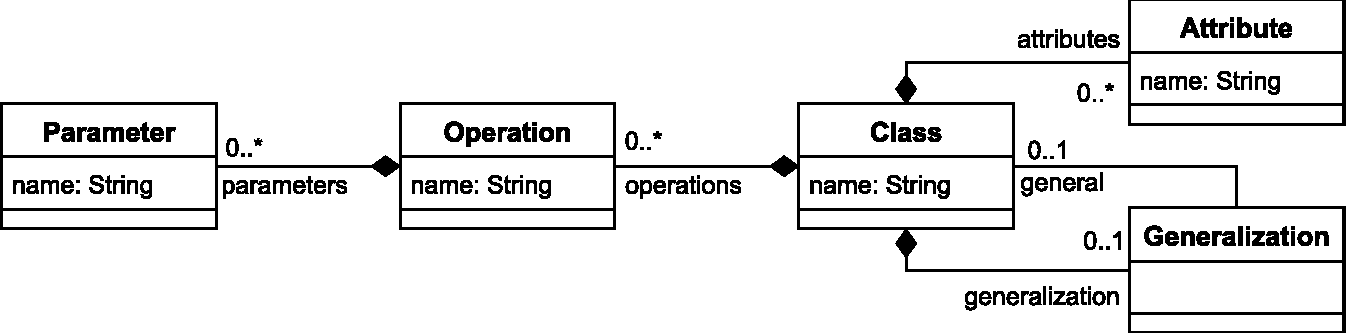
\includegraphics[width=\linewidth]{miniuml_metamodel}
  \caption{An excerpt of the UML-like meta-model of the running example in Figure \ref{fig:class_diagram_rpg}.}
  \label{fig:miniuml_metamodel}
\end{figure*}

\begin{figure*}[h]
  \centering
  \begin{subfigure}[t]{0.47\linewidth}
    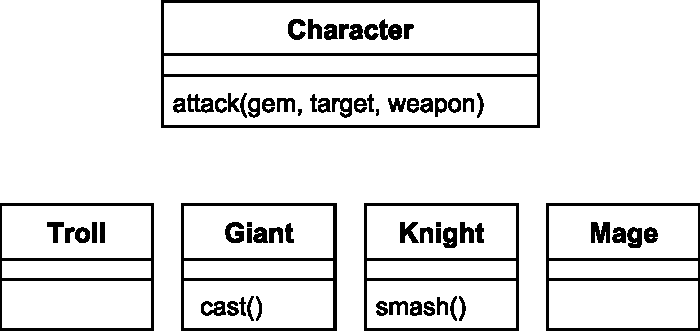
\includegraphics[width=\linewidth]{class_diagram_origin}
    \caption{original version (Jane’s version)}
    \label{fig:class_diagram_origin}
  \end{subfigure}
  \\
  \begin{subfigure}[t]{0.47\linewidth}
    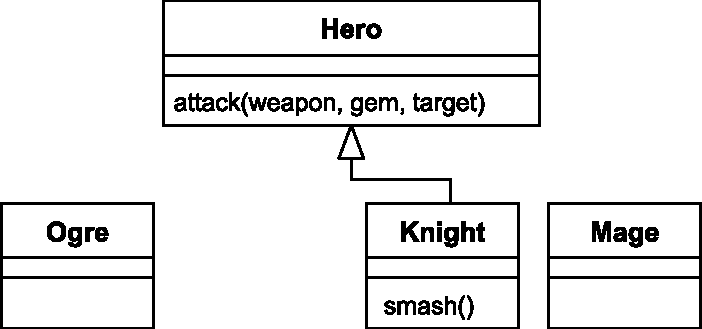
\includegraphics[width=\linewidth]{class_diagram_left}
    \caption{left version (Bob’s version)}
    \label{fig:class_diagram_left}
  \end{subfigure}
  \hfill
  \begin{subfigure}[t]{0.47\linewidth}
    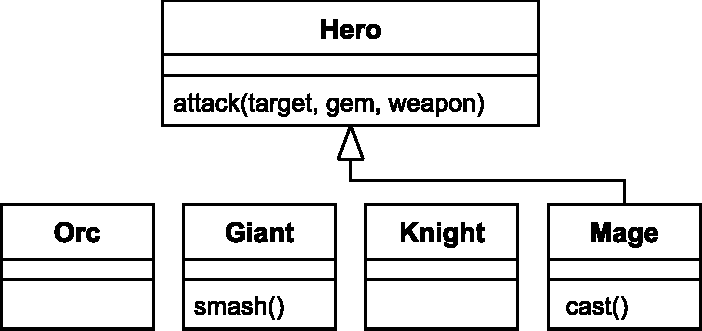
\includegraphics[width=\linewidth]{class_diagram_right}
    \caption{right version (Alice’s version)}
    \label{fig:class_diagram_right}
  \end{subfigure}
  \caption{Three incomplete class diagrams of a Role Playing Game.}
  \label{fig:class_diagram_rpg}
\end{figure*}

In this scenario, Jane has set up an initial model of a Role Playing Game (RPG) (Figure \ref{fig:class_diagram_origin}). She then assigned this work to Bob and Alice. Both Alice and Bob continued to work on the model and made some modifications, seen in Figures \ref{fig:class_diagram_left} and \ref{fig:class_diagram_right} respectively. Persisting these models in the standard XMI \cite{omg2018xmi} format produces three files as shown in Listings \ref{lst:xmimodel_origin}, \ref{lst:xmimodel_left}, and \ref{lst:xmimodel_right}. In this running example, every element has its globally unique ID. Thus, if Bob and Alice create two elements independently, they will not be allocated the same ID. For example, the generalisations that Bob and Alice added in Listings \ref{lst:xmimodel_left} and \ref{lst:xmimodel_right} have different IDs, \textsf{leftGen} and \textsf{rightGen} respectively.

An alternative way to persist these three models would be to persist the sequence of all changes through which they were constructed, not to persist their state. This approach was first introduced in \cite{DBLP:conf/models/YohannisKP17}, and it is illustrated in the next section. This example is extended in Section \ref{sec:runnnig_example_continue} to facilitate explaining the change-based model differencing proposed in this research.

\section{Proposed Approach}
\label{sec:proposed_approach}

To illustrate the proposed approach, Listing \ref{lst:xmimodel_left} shows a state-based representation of Bob’s model in Figure \ref{fig:class_diagram_left} in (simplified) XMI, and Listing \ref{lst:cbp_left_full} shows the proposed equivalent change-based representation of the same model. Instead of persisting a snapshot of the model’s state, the representation of Listing \ref{lst:cbp_left_full} captures the complete sequence of change events (create/set/add/move/remove/delete) that were performed on the model since its creation, organised in editing sessions. There are two editing session in the case of this model. The session at line 1 marks the editing made by Jane until line 29. Replaying these changes produces Jane’s model in Figure \ref{fig:class_diagram_origin}. The rest of the change events are the modification performed by Bob on Jane’s model. Replaying all the changes, both Jane’s and Bob’s changes, produces the same state as the one captured in Listing \ref{lst:xmimodel_left} or Figure \ref{fig:class_diagram_left}. Thus, we can conclude that the proposed change-based representation carries at least as much information as the state-based representation.

\vspace{-20pt}
\begin{lstlisting}[style=eol,float=tp,escapechar=|,caption={The complete change events of Bob’s model in Figure \ref{fig:class_diagram_left}.},label=lst:cbp_left_full]
session "Jane-01"
create character type Class
set character.name from null to "Character"
create attack type Operation
set attack.name from null to "attack"
add attack to character.operations at 0
create gem type Parameter
set gem.name from null to "gem"
add gem to attack.parameters at 0
create target type Parameter
set target.name from null to "target"
add target to attack.parameters at 1
create weapon type Parameter
set weapon.name from null to "weapon"
add weapon to attack.parameters at 2
create troll type Class
set troll.name from null to "Troll"
create giant type class
set giant.name from null to "Giant"
create cast type Operation
set cast.name from null to "smash"
add cast to giant.operations at 0
create knight type Class
set knight.name from null to "Knight"
create smash type Operation
set smash.name from null to "smash"
add smash to knight.operations at 0
create mage type Class
set mage.name from null to "Mage"
session "Bob-01"
create leftGen type Generalization
set leftGen.general from null to character
set troll.generalization to leftGen
set character.name from "Character" to "Hero"
unset troll.generalization from leftGen to null composite l1
set knight.generalization to leftGen composite l1
move target in attack.parameters from 1 to 2
unset cast.name from "cast" to null composite l2
remove cast from giant.operations at 0 composite l2
delete cast composite l2
unset giant.name from "Giant" to null composite l2
delete giant composite l2
set troll.name from "Troll" to "Ogre"
\end{lstlisting}

Such a representation is particularly suitable to identify the changes of the model since the last version. For example, if we can identify that changes recorded for the previous version came before editing session \textsf{Bob-01} (lines 1–29) of the model, we can readily identify the changes that were made to the model since then (i.e. in session \textsf{Bob-01}—lines 30–43) instead of having to rediscover them through expensive state-based model differencing.

For the sake of readability, the format of change-based persistence presented in Listing \ref{lst:cbp_left_full} is a simplified version. The real format is in XML-like-format (Appendix \ref{lst:class_diagram_left_cbpfile}). For example, change event \textsf{session "Jane-01"} is persisted as:

\textsf{<session ID="Jane-01" time="20190923181841687GMT"/>}

and \textsf{set character.name from null to "Character"} is persisted as:

\textsf{<set-eattribute eclass="Class" name="name"
  target = "character">
  <old-value literal=null/>
  <value literal = "Character"/>
  </set-eattribute>}.

Change events that have been persisted to a change-based persistence file cannot be altered or removed. They are immutable. Only new change events can be appended to the file.

%\section{Requirements}
%\label{sec:requirements}
%From the literature review and the text-based change summaries in the above listings, a number of requirements have been gathered as guidance for designing the implementation of change-based persistence.
%\begin{enumerate}
% \item[R1] The implementation should be able to listen and collect change events when a model is modified.
% \item[R2] It should conform to model and meta-model infrastructure of the Eclipse Modeling Framework.
% \item[R3] A change event should contain necessary information, such as change event type (add, remove, delete, create, set, unset, composite), element (class and ID), feature (name and type), value (literal or object), and index (from and to), so that when replaying them orderly an equivalent model is constructed.
% \item[R4] The implementation should be able to append change events into a change-based model file as well as to (re)load them from the file by replaying all the change events.
%\end{enumerate}

\section{Prototype Implementation}
\label{sec:prototype_implementation}

A prototype \cite{epsilonlabs2019emfcbp} of the change-based model persistence format (EMF CBP) has been implemented using the model-element level change notification facilities provided by the Eclipse Modeling Framework. In that implementation, the prototype uses a subclass of EMF’s \textsf{EContentAdapter} (\textsf{ChangeEventAdapter}) to receive and record \textsf{Notification} events produced by the framework for every model-element-level change.

\begin{figure*}[th]
  \centering
  \includegraphics[width=\linewidth]{events}
  \caption{Event classes to represent changes of models.}
  \label{fig:events}
\end{figure*}

Since not all change events are relevant to change-based persistence (e.g. EMF also produces change notifications when listeners/adapted are added/removed from the model), we have defined a set of event classes to represent events of interest. The event classes are depicted in Figure \ref{fig:events} as subclasses of the \textsf{ChangeEvent} abstract class.

EMF has dedicated classes to express the graph structure of a model. For instance, \textsf{EStructuralFeature} can be \textsf{EReference} or \textsf{EAttribute}, it can have a single value or multiple values (e.g., Integer, String), the value(s) of \textsf{EStructuralFeature} can be a \textsf{EObject} or primitive, the \textsf{EReference} can be a containment or non-containment. These characteristics drive the design of the prototype to have different subclasses of \textsf{ChangeEvent}, and they also decide which attributes and methods should be defined in the class.

The \textsf{ChangeEvent} class has a multi-valued \textsf{values} attribute, which can accommodate both single-valued (e.g. set/add) or multi-valued events (e.g. addAll/removeAll). \textsf{ChangeEvent} can also accommodate different types of values, such as \textsf{EObject}s for \textsf{EReferenceEvents} and primitive values (e.g. Integer, String) for \textsf{EAttributeEvents}. The \textsf{ChangeEvent} class also has a position attribute to hold the index of an \textsf{EObject} or a literal when they are added to a \textsf{Resource}, \textsf{EReference}, or \textsf{EAttribute} with multiple values.

Every time an \textsf{EObject} is added to the model, a globally unique ID is assigned to the \textsf{EObject}, and a \textsf{CreateEObjectEvent} and an \textsf{AddToResourceEvent} are recorded. When an EObject is deleted, or moved to a containment \textsf{EReference} elsewhere in the model, a \textsf{RemoveFromResourceEvent} is recorded.

\begin{lstlisting}[style=java,caption={Simplified Java code to handle notification events.},label=lst:javacode]
public class ChangeEventAdapter extends EContentAdapter {
  ...
  @override
  public void notifyChanged(Notification n) {
  ...
  switch (n.getEventType()) {
    ... // other events
    case Notification.UNSET: {
      if (n.getNotifier() instanceof EObject) {
        EStructuralFeature feature = (EStructuralFeature) n.getFeature();
        if (feature instanceof EAttribute) {
          event = new UnsetEAttributeEvent();
        } else if (feature instanceof EReference) {
          event = new UnsetEReferenceEvent();
        }
      } break;
    }
    ... // other events
\end{lstlisting}	

The \textsf{ChangeEventAdapter} receives EMF change notifications in its \textsf{notifyChanged()} method and filters and transforms them into appropriate change events. As an example of how notifications are filtered and transformed, Listing \ref{lst:javacode} shows how the prototype handles \textsf{Notification.UNSET} events, based on the type of the feature that was changed. That is, an \textsf{UnsetEAttributeEvent} is instantiated if the feature of the notifier is an \textsf{EAttribute}, or an \textsf{UnsetEReferenceEvent} is created if the notifier is an \textsf{EReference}. The transformed instances are then stored in a list of events in \textsf{ChangeEventAdapter} (\textsf{ChangeEvents}) for persistence.

To integrate seamlessly with the EMF framework and to eventually support multiple concrete change-based serialisation formats (e.g. XML-formatted representation for readability and binary for performance/size), the prototype implemented a \textsf{CBPResource} abstract class that extends EMF’s built-in \textsf{ResourceImpl} class. The role of the abstract class is to encapsulate all change recording functionality while the role of its concrete subclasses is to implement serialisation and de-serialisation.
To save a model, \textsf{CBPXMLResourceImpl} persists changes in a line-based format where every change is serialised as a single-line XML document. In this way, when a model changes, the prototype can append the new changes to the end of the model file without needing to serialise the entire model again.
To load a model, \textsf{CBPXMLResourceImpl} de-serialises every line in the document as a change event and then re-executes it to reconstruct the model.
The prototype also includes a \textsf{CBPXMLResourceFactory} class that extends EMF’s \textsf{ResourceFactoryImpl} as the factory class for change-based models. Figure \ref{fig:resources} shows the relationships between these classes.format 

\begin{figure}[th]
  \centering
  \includegraphics[width=\linewidth]{resources}
  \caption{Factory, resource, and ChangeEventAdapter classes.}
  \label{fig:resources}
\end{figure}

Listing \ref{lst:javacode_resource} shows how to use the prototype in Java code. Lines 1–8 demonstrate how to initialise and save a model using the prototype. First, the code creates an instance of \textsf{CBPResource}, \textsf{cbpResource}, using \textsf{CBPXMLResourceFactory} and specifies its file as \textsf{helloworld.cbpxml} using \textsf{URI}. The code then executes method \textsf{startNewSession} of \textsf{cbpResource}. This method adds a change event to indicate the start of the editing session as depicted at line 1 in Listings \ref{lst:cbp_origin} and \ref{lst:cbp_left}.
The code then uses \textsf{UMLFactory} to create an element, \textsf{model}, of UML2’s \textsf{Model}. The code adds \textsf{model} into \textsf{cbpResource} and sets the name to ‘Hello World’. The code then saves the model in change-based format using \textsf{save} and then unloads \textsf{cbpResource}. Lines 9–12 demonstrate how to replay (load) the model that had been saved and then print the name of the first element in \textsf{cbpResource}, which is expected to print “Hello World”.

\vspace{-20pt}
\begin{lstlisting}[style=java,caption={An example how to use \textsf{CBPResource} in Java code.},label=lst:javacode_resource]
/* initialise, save, and unload */
CBPResource = (CBPResource) (new CBPXMLResourceFactory()).createResource(URI.createFileURI("helloworld.cbpxml"));
cbpResource.startNewSession("Initial");
Model = UMLFactory.eINSTANCE.createModel();
cbpResource.getContents().add(model);
model.setName("Hello World");
cbpResource.save(null);
cbpResource.unload();

/* load and print */
cbpResource.load(null);
model = (Model) cbpResource.getContents().get(0);
System.out.println(model.getName()); // expected output: "Hello World"
\end{lstlisting}

%\section{Benefits and Novel Capabilities}
%\label{sec:benefits_and_novel_capabilities}
%This section highlights some of the benefitsnovel capabilities of the prototype.
%
%\begin{itemize}
%\item With appropriate tool support, modellers will be able to ‘replay’ (part of) the change history of a model (e.g. to understand design decisions made by other developers, for training purposes). In state-based approaches, this can be partly achieved if models are stored in a version control repository (e.g. Git). However, the granularity would be at the commit level only.
%\item By analysing models serialised in the proposed representation, modelling language and tool vendors will be able to develop deeper insights into how modellers use these languages/tools in practice. They can then use this information to guide the evolution of the language/tool. An early work for this case is in \cite{polack2019towards}.
%\item By attaching additional information to each session (e.g. the ID of the developer, references to external documents/URLs), sequences of changes can be traced back to the developer that made them or to the requirements/bug reports that triggered them.
%\item Persisting changes to large models after an editing session will be significantly faster than serialising the entire state of the model, as only changes made during the session will need to be appended to the model file. The evaluation of this benefit can be found in Chapters \ref{ch:optimised_loading} and \ref{ch:hybrid_model_persistence} of this thesis.
%\item The performance and precision of model differencing and conflict detection can be substantially improved, particularly for large models with shared editing histories. The evaluation of this benefit can be found in Chapters \ref{ch:model_differencing} and \ref{ch:conflict_detection} of this thesis.
%\item Using a text file to persist changes of a model allows common text-oriented version controls, such as Git and SVN, to be used for model versioning. Text-oriented version controls are not supported by EMF Store—an existing implementation of change-based persistence of EMF models—which uses its own mechanism to version models.
%\end{itemize}

\section{Challenges}
\label{sec:challenges}
This section highlights the challenges that come from adopting change-based persistence. As was mentioned in the literature review, change-based persistence also comes with a number of challenges, such as (1) loading overhead and (2) fast-growing model files, which can hold back the delivery of its potential benefits. Addressing these challenges surely facilitates its adoption.

For the first challenge, persisting changes to large models is expected to be much faster and resource-efficient than state-based approaches, since loading models into memory by naïvely replaying the entire change history is expected to have a significant overhead. This work has addressed this challenge by proposing two solutions that reduce the cost of change-based model loading. The first solution is to record and ignore events that are later overridden or cancelled out by other events. That solution can be found in Chapter \ref{ch:optimised_loading}. The second solution is a proposed hybrid model persistence format that uses change-based and state-based persistence together. In that solution, changes applied to a model are persisted into both change-based and state-based representations, but the model is loaded from the stated-based persistence. In that way, it avoids replaying the change events. This solution is discussed in Chapter \ref{ch:hybrid_model_persistence}.

In the second challenge—fast-growing model files—persisting a model in a change-based format means that the size of its file grows significantly faster during the model’s evolution than it does in its state-based counterpart. This challenge has not been addressed in this research, and must be considered in future work. Nevertheless, this research recommends two solutions. Use sound change-compression operations (e.g. remove older/unused information) to reduce the size of a model in a controlled way, or develop  a compact textual format that will minimise the space required to record a change. (A textual line-separated format is desirable to maintain compatibility with file-based version control systems.)

\section{Conclusions}
\label{sec:conclusions_3}
Through persisting models’ change history, this research aims to enable high-performance model differencing and conflict detection in collaborative development settings. This study has translated the concept of change-based persistence into an implementation in a modelling framework, which can be used to persist models.

In this chapter, a running example was introduced. This example is used throughout this thesis to explain the solutions proposed in this study. A prototype of a change-based persistence format also was presented, including its requirements and a design of the implementation that meets the requirements. Some potential benefits and novel capabilities that a change-based persistence can contribute and the challenges that might restrain delivering them also have been presented.

This chapter also has partially addressed the first research question of this study, \textbf{How can models be persisted in a change-based format, and how does change-based persistence perform, compared to state-based persistence, in terms of loading and saving models?} (RQ1). To persist models in a change-based format, a prototype has been developed. It captures relevant notifications returned by the notification facilities provided by EMF every time a change is applied to an EMF model. It then transforms the notifications into different classes of change events representing different types of changes (e.g., set, unset, add, remove, move, create, and delete) that conform to the model and meta-model infrastructure of EMF. Every captured change event is then persisted by appending it into an XML-like-formatted file when the model is saved. The model can be (re)loaded by de-serialising the file and (re)executing all the persisted change events—replaying the historical construction of the model. Please refer to Appendix \ref{sec:reproducing_experiments} to download the source code of the prototype.


\chapter{Optimised Loading of Change-based Model Persistence}
\label{ch:optimised_loading}

This chapter introduces and evaluates an efficient approach for loading models stored in a change-based format. This work builds on the change-based model persistence format presented in Chapter 3. It also presents an evaluation on the performance of the proposed loading approach and an assessment of its impact on saving change-based models. The results show that the proposed approach significantly improves loading times compared to the baseline change-based persistence loading approach, and it has a negligible impact on saving.

\section{Introduction}
\label{sec:introduction_4}
Saving a model in change-based persistence typically results in a large, ever-increasing file (see Table \ref{table:advantages_drawbacks}) since every change made to the model (even model element deletions) is appended to the file. This also applies to the implementation of change-based model persistence (CBP) in this work, which uses a text file to simplify saving changes by appending them and reading them into memory. The increasing records of changes also cause the loading time of the model to increase, as the loading process has to reconstruct the model’s current state from its history \cite{DBLP:conf/models/YohannisKP17}. This chapter proposes and evaluates an approach that reduces CBP model loading time by avoiding the replaying of historical changes that have no impact on the final state of the model.

The rest of this chapter is structured as follows. Section \ref{sec:case_study} introduces a running example.
Section \ref{sec:loading_time_optimisation} presents the proposed approach to speed up model loading and its supporting data structures. Section \ref{sec:evaluation_4} presents experimental results and evaluation. Section \ref{sec:conclusions_4} concludes this chapter.

\section{Running Example}
\label{sec:case_study}
To explain the optimised loading algorithm for change-based models, this chapter uses the minimal tree meta-model and example tree models in Figure \ref{fig:tree_example}.

The meta-model for the minimal tree model is expressed in the Eclipse Modeling Framework (EMF) Ecore meta-modelling language, the de-facto standard for object-oriented meta-modelling. The example is contrived to avoid unnecessary repetition, while providing adequate coverage of the core features of Ecore (classes, single/multi-valued features, references).
In this example, a tree model consists of named nodes which can—optionally—contain other nodes (\textsf{child} reference).

\begin{figure}[ht]
  \begin{subfigure}[t]{0.32\linewidth}
    \centering
    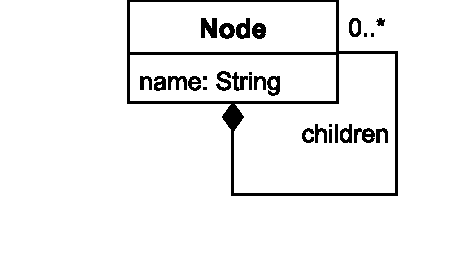
\includegraphics[width=\linewidth]{node_metamodel}
    \caption{the tree meta-model (EMF/Ecore)}
    \label{fig:tree_metamodel}
  \end{subfigure}
  \hfill
  \begin{subfigure}[t]{0.32\linewidth}
    \centering
    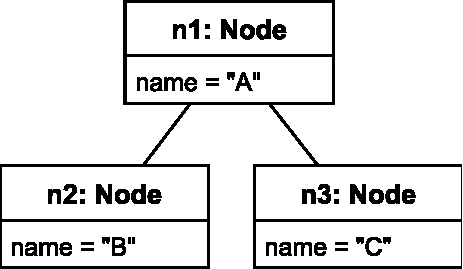
\includegraphics[width=\linewidth]{initial_chart_1}
    \caption{the initial state of a tree model}
    \label{fig:initial_model}
  \end{subfigure}
  \hfill
  \begin{subfigure}[t]{0.32\linewidth}
    \centering
    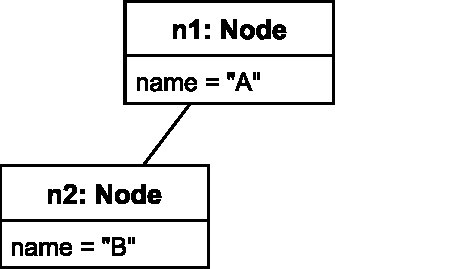
\includegraphics[width=\linewidth]{initial_chart_2}
    \caption{the eventual state after \textsf{n3} is deleted}
    \label{fig:modified_model}
  \end{subfigure}
  \caption{Running example of a meta-model and a conformant model.}
  \label{fig:tree_example}
\end{figure}

The initial state of the model in Figure \ref{fig:initial_model} has three nodes, \textsf{n1}, \textsf{n2}, and \textsf{n3}. It was initially constructed by creating the three nodes (\textsf{n1}, \textsf{n2}, and \textsf{n3}), and nodes \textsf{n2} and \textsf{n3} were added as children of \textsf{n1}. The model was modified by deleting node \textsf{n3} producing the eventual state in Figure \ref{fig:modified_model}.

\vspace{-20pt}
\begin{minipage}[t]{0.49\linewidth}
\begin{lstlisting}[style=xmi,caption={State-based representation in simplified XMI of the tree model in Figure \ref{fig:initial_model}.},label=lst:xmimodel_0]
<Node id="n1" name="A">
  <children id="n2" name="B"/>
  <children id="n3" name="C"/>
</Node>
\end{lstlisting}
\end{minipage}
\hfill
\begin{minipage}[t]{0.49\linewidth}
\begin{lstlisting}[style=xmi,caption={State-based representation in simplified XMI of the tree model in Figure \ref{fig:modified_model}.},label=lst:xmimodel]
<Node id="n1" name="A">
  <children id="n2" name="B"/>
</Node>
\end{lstlisting}
\end{minipage}

\vspace{-20pt}
\begin{minipage}[t]{0.49\linewidth}
\begin{lstlisting}[style=eol,caption={Change-based representation of the tree model in Figure \ref{fig:initial_model}.},label=lst:cbpmodel_0]
create n1 of Node
set n1.name from null to "A"
create n2 of Node
set n2.name from null to "B"
create n3 of Node
set n3.name from null to "C"
add n2 to n1.children at 0
add n3 to n1.children at 1
\end{lstlisting}
\end{minipage}
\hfill
\begin{minipage}[t]{0.49\linewidth}
\begin{lstlisting}[style=eol,caption={Change-based representation of the tree model in Figure \ref{fig:modified_model}.},label=lst:cbpmodel]
create n1 of Node
set n1.name from null to "A"
create n2 of Node
set n2.name from null to "B"
create n3 of Node
set n3.name from null to "C"
add n2 to n1.children at 0
add n3 to n1.children at 1
remove n3 from n1.children at 1
delete n3
\end{lstlisting}
\end{minipage}

Listings \ref{lst:xmimodel_0} and \ref{lst:xmimodel} show the simplified XMI format of the models in Figures \ref{fig:initial_model} and \ref{fig:modified_model} when they are persisted in state-based representation. Listings \ref{lst:cbpmodel_0} and \ref{lst:cbpmodel} show the change-based representation of the two models respectively, using the CBP syntax introduced in Chapter \ref{ch:change_based_model_persistence}. As both change-based representations show, lines 1–6 record the creation and naming of the three nodes, and lines 7–8 record the addition of \textsf{n2} and \textsf{n3} as children of \textsf{n1}. Change-based representation in Listing \ref{lst:cbpmodel} records two additional rows since it also records the recent changes that produce the eventual state of the tree model in Figure \ref{fig:modified_model}. Lines 9–10 capture the deletion of \textsf{n3} (the \textsf{remove} command removes f \textsf{n3} from its container, and the $delete$ command completely removes \textsf{n3} from its model). Changes in a CBP representation can be uniquely identified by their line numbers.

This example model history illustrates a case where earlier events (creating \textsf{n3} in line 5, naming it in line 6, making it a child of \textsf{n1} in line 8, and removing it from the container in line 9) are superseded by a subsequent event (deletion of \textsf{n3} in line 10). Loading the eventual model would arguably be faster if the events in lines 5, 6, 8, 9, and 10 could be ignored.

%\vspace{-10pt}
\section{Toward Efficient Loading of Change-Based Models}
\label{sec:loading_time_optimisation}

%\vspace{-10pt}
The flowchart in Figure \ref{fig:flowchart} provides an overview of the editing lifecycle of a CBP model \cite{DBLP:conf/models/YohannisKP17}, with the proposed extensions shown as starred blocks. A model is loaded (1), edited (2), and saved (3). During editing, the changes made to the model are recorded in a memory-based data structure, serialised, and, with the latest events, appended at the end (4). The change events are persisted into a CBP file every time the model is saved (5). When a model is reloaded, the current model state is recreated by replaying the events stored in the CBP file (6).

\begin{figure}[ht]
  \centering
  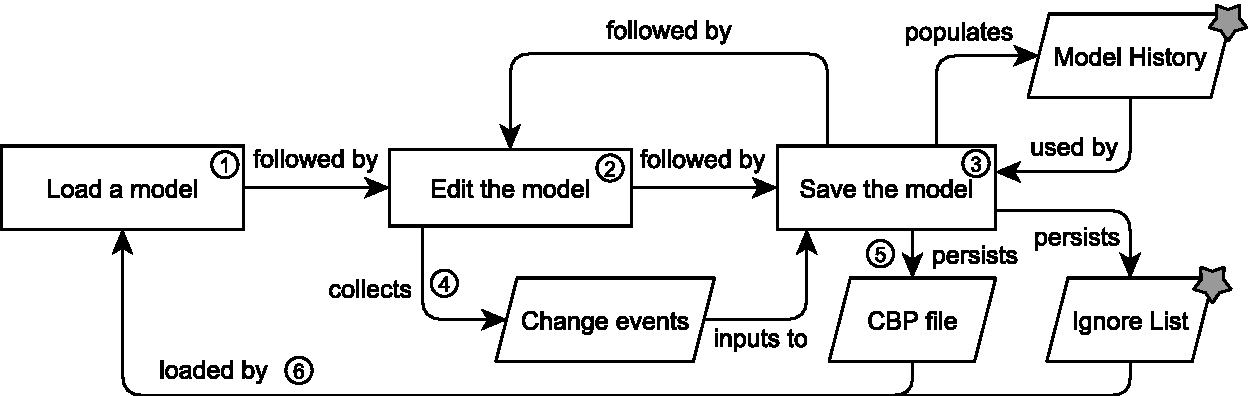
\includegraphics[width=\linewidth]{flowchart}
  \caption{CBP workflow, with optimised loading elements indicated by starred blocks.}
  \label{fig:flowchart}
\end{figure}

As mentioned in Section \ref{sec:proposed_approach}, the editing history recorded in a CBP file is immutable. As such, superseded events cannot be simply removed from the CBP file. Therefore, the proposed approach adds two artefacts: an in-memory \textit{Model History} data structure, which aggregates change events per model element, and an \textit{Ignore List} file, which persists the position (i.e. line numbers) of superseded events so that the events can be ignored the next time the model is loaded. The Ignore List is saved alongside the CBP file. The rest of this section presents how the Model History is used to detect superseded events and generate the Ignore List.

\subsection{Model History}
\label{subsec:model_history}
The Model History data structure stores events and their line numbers in a CBP representation. The data can be used to reason about the events of a particular element and to determine which events are superseded. The line number in the CBP representation is referred as the \textit{event number}. The proposed data structure is defined in Figure \ref{fig:object_history} using a class diagram.

A \textsf{ModelHistory} has a \textsf{URI} attribute to identify the model for which it records changes. A \textsf{ModelHistory} can link to many \textsf{ElementHistory} objects, each identified by its \textsf{element} field, which is queried from the model. An \textsf{ElementHistory} can link to many \textsf{FeatureHistories}, representing the editing histories of individual features—either references or attributes of the element. A \textsf{FeatureHistory} has a \textsf{type} (attribute or reference) and a \textsf{name}, identifying the feature.

%\vspace{-20pt}
\begin{figure}[ht]
  \centering
  \includegraphics[width=\linewidth]{object_history}
  \caption{The class model defining Model History.}
  \label{fig:object_history}
\end{figure}

%\vspace{-30pt}
\begin{figure}[ht]
  \centering
  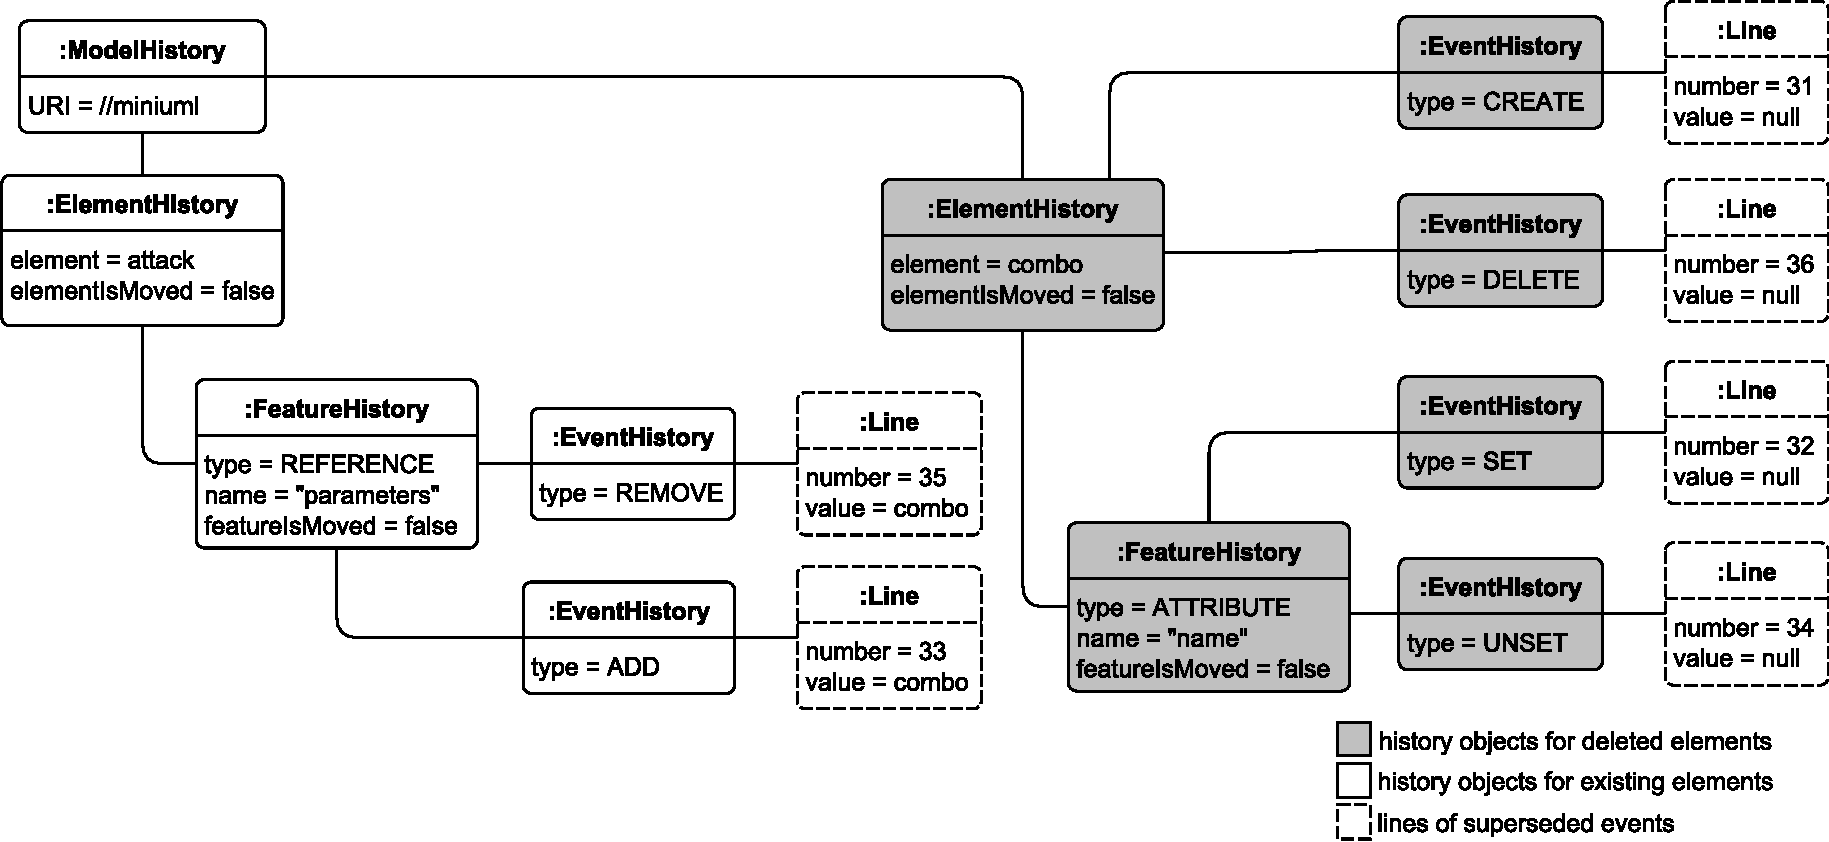
\includegraphics[width=\linewidth]{history_structure}
  \caption{The object diagram of the CBP model history in Listing \ref{lst:cbpmodel}.}
  \label{fig:history_structure}
\end{figure}

An \textsf{EventHistory} represents a series of events of the same type; it has an attribute \textsf{type} to identify the events’ type and can have many \textsf{Line}s. A \textsf{Line} has a \textsf{number} attribute to record the event number and a \textsf{value} that records the element involved in the event (Value is only used for events with types \textsf{add}, \textsf{remove}, and \textsf{move}). Each \textsf{FeatureHistory} can have many \textsf{EventHistories} to represent events that modify the values of the features. Each \textsf{ElementHistory} can have many \textsf{EventHistories} to represent events that affect the state of the elements (life-cycle and relations to multi-valued features). Figure \ref{fig:history_structure} shows an object diagram corresponding to the model in Figure \ref{fig:object_history}, which captures the model history shown in Listing \ref{lst:cbpmodel}. The grey rectangles are \textsf{History} objects related to the deleted node \textsf{n3}. The rectangles with dashed outlines are \textsf{Line} objects that represent superseded changes.

The following section presents the different strategies used to identify superseded events that will be added to the Ignore List.

%\vspace{-10pt}
\subsection{Set and Unset Events}
\label{subsec:set_and_unset_operations}
During the lifecycle of a model, a single-valued feature can have its value set (assigned) or unset many times. Each event is persisted, but only the last assigned value needs to be considered. For example, in Listing \ref{lst:set_unset_example_1}, the feature \textsf{name} is set to the value “A”, unset, and finally set to the value “B”. In the final state of the model, \textsf{n1.name} = “B”. Thus, only line 4 is significant for the model’s final state and therefore lines 2 and 3 can be ignored when loading the model. For a \textsf{set} event, all preceding \textsf{set} and \textsf{unset} events can be ignored, but for an \textsf{unset} event, all \textsf{set} and \textsf{unset} events can be ignored. Executing it does not have any effect on the final state of a model if all the preceding events also have been ignored.

\vspace{-20pt}
\begin{minipage}[t]{0.49\linewidth}
\begin{lstlisting}[style=eol,caption={A CBP representation of attribute \textsf{name} assignments ended with SET.},label=lst:set_unset_example_1]
create n1 of Node
set n1.name from null to "A"
unset n1.name from "A" to null
set n1.name from null to "B"
\end{lstlisting}
\end{minipage}
\hfill
\begin{minipage}[t]{0.49\linewidth}
\begin{lstlisting}[style=eol,caption={A CBP representation of attribute \textsf{name} assignments ended with UNSET.},label=lst:set_unset_example_2]
create n1 of Node
set n1.name from null to "A"
set n1.name from null to "B"
unset n1.name from "B" to null
\end{lstlisting}
\end{minipage}

Based on Listing \ref{lst:set_unset_example_1}, our approach creates an instance of \textsf{ElementHistory} \textsf{n1}, which contains an instance of \textsf{FeatureHistory} \textsf{name}. The \textsf{FeatureHistory} \textsf{name} consists of two \textsf{EventHistory} instances, with types \textsf{set} and \textsf{unset} (the instances are named \textsf{set} and \textsf{unset} respectively for brevity). The \textsf{set} records the $Line$ instances that hold the event numbers of the \textsf{set} events, and similarly for \textsf{unset}.

From Listing \ref{lst:set_unset_example_1}, we can thus infer that \textsf{name}.\textsf{set}.\textsf{lines} = $\{2,4\}$ and \textsf{name}.\textsf{unset}. \textsf{lines} = $\{3\}$. The event numbers in both lists are used to determine that the events represented by lines 2 and 3 are superseded by the event in line 4, which is a \textsf{set} event, giving an \textsf{ignoreList} = $\{2, 3\}$. By the same process, for Listing \ref{lst:set_unset_example_2}, we can reason that \textsf{name}.\textsf{set}.\textsf{lines} = \{2,3\} and \textsf{name}.\textsf{unset}.\textsf{lines} = \{4\}. However, in this case, the highest-numbered event is an \textsf{unset}, all so line numbers are put into the Ignore List (\textsf{ignoreList} = $\{2, 3, 4\}$) (\textsf{unset} event can be ignored along with all preceding {\textsf{set} and \textsf{unset} events).
  
  %\vspace{-10pt}
  \subsection{Add, Remove, and Move Events}\label{subsec:add_remove_and_move_operations}
  For a multi-valued feature, add, remove, and move events can be called many times to modify the feature. If an element is added to the feature, moved multiple times, and finally removed, then all the element’s preceding events can be ignored, as long as the order of the feature’s elements is not changed.
  
  Listing \ref{lst:add_move_reference} shows an example without a \textsf{move} event. In this example, nodes \textsf{n1}, \textsf{n2}, and \textsf{n3} are added to the \textsf{children} feature of \textsf{p} (lines 5–7). In the latest state of the model, \textsf{children} only contains \textsf{n1} and \textsf{n3}. As a result, the loading process could ignore the events that represent the \textsf{add} and \textsf{remove} events on \textsf{n1}.
  
\vspace{-20pt}
\begin{lstlisting}[style=eol,caption={A CBP of add and remove operations.},label=lst:add_move_reference]
create p of Node // children = []
create n1 of Node // children = []
create n2 of Node // children = []
create n3 of Node // children = []
add n1 to p.children at 0 // children = [n1]
add n2 to p.children at 1 // children = [n1, n2]
add n3 to p.children at 2 // children = [n1, n2, n3]
remove n2 from p.children at 1 // children = [n1, n3]
\end{lstlisting}

\begin{lstlisting}[style=eol,caption={A CBP representation of add, move, and remove operations.},label=lst:add_remove_move_reference]
create p of Node // children = []
create n1 of Node // children = []
create n2 of Node // children = []
create n3 of Node // children = []
add n1 to p.children at 0 // children = [n1]
add n2 to p.children at 1 // children = [n1, n2]
add n3 to p.children at 2 // children = [n1, n2, n3]
move n1 in p.children from 0 to 1 // children = [n2, n1, n3]
remove n2 from p.children at 0 // children = [n1, n3]
\end{lstlisting}
  
  To create the Ignore List for Listing \ref{lst:add_move_reference}, we can deduce that \textsf{children}.\textsf{add}.\textsf{lines} = \{\{5, \textsf{n1}\}, \{6, \textsf{n2}\}, \{7, \textsf{n3}\}\} (5 is the line number and \textsf{n1} is the value) and \textsf{children}.\textsf{remove}.\textsf{lines} = \{\{8, \textsf{n1}\}\}. Since \textsf{n2} is removed from its containing feature (line 8), then executing its preceding add and remove events is unnecessary. Note that we retain the \textsf{create} event (line 3) as \textsf{n2} has not been deleted from the model—only removed from its containing feature. We can iterate through the add and move structures to identify the events on \textsf{n2} that should be removed, resulting in the \textsf{ignoreList} = \{6, 8\}.
  
  Listing \ref{lst:add_remove_move_reference} shows an example with a \textsf{move} event\footnote{The commented parts show the end states of \textsf{children} after each event}. Let’s say that a \textsf{move} event is inserted at line 8 (this insertion shifts the \textsf{remove} event of \textsf{n2} from line 8 to line 9). With the introduction of this \textsf{move} event, we now have the \textsf{children}.\textsf{add}.\textsf{lines} = \{\{5, \textsf{n1}\}, \{6, \textsf{n2}\}, \{7, \textsf{n3}\}\}, \textsf{children}.\textsf{move}.\textsf{lines} = \{\{8, \textsf{n1}\}\}, and \textsf{children}.\textsf{remove}.\textsf{lines} = \{\{9, \textsf{n2}\}\}. In the final state of the model, \textsf{children} should have \textsf{n1} and \textsf{n3} in order, \textsf{children} = [n1, n3].
  
  However, executing the previous strategy naïvely leads to an erroneous final state. Using \textsf{ignoreList} = \{6, 8\} produced by the naïve strategy leads to a different order of \textsf{n1} and \textsf{n3} in the final state of the model where \textsf{children} = [n3, n1] as shown by the naïve optimised CBP in Listing \ref{lst:naive_add_remove_move_reference}. To overcome this problem, *$IsMoved$ flags in Figure \ref{fig:object_history} are used to sign features and elements. If they have been moved—the flags are set to $true$. If an element’s *$IsMoved$ flag is true, then all of its line numbers related to \textsf{add}, \textsf{move}, \textsf{remove} events cannot be put into the \textsf{ignoreList}. The flags are set to $false$ if the feature is empty.
  
\vspace{-20pt}
\begin{lstlisting}[style=eol,caption={A naïve optimised CBP representation of original CBP representation in Listing \ref{lst:add_remove_move_reference}}, label=lst:naive_add_remove_move_reference]
create p of Node // children = []
create n1 of Node // children = []
create n2 of Node // children = []
create n3 of Node // children = []
add n1 to p.children at 0 // children = [n1]
add n3 to p.children at 1 // children = [n1, n3]
move n1 in p.children from 0 to 1 // children = [n3, n1]
\end{lstlisting}
  
  \subsection{Create and Delete Events}
  \label{subsec:create_and_delete_operations}
  
  When an element is deleted, it is completely removed from the model. Therefore, all previous events ($create$, \textsf{set}, \textsf{unset}, \textsf{move}, \textsf{add}, \textsf{remove}, $delete$) on features of the element can be ignored. For example, when node \textsf{n3} in Listing \ref{lst:cbpmodel} is deleted, the events in lines 5–6 and 8–10 are superseded. If Listing \ref{lst:cbpmodel} is optimised—some of its events are ignored—when loading, it runs as if Listing \ref{lst:cbpmodel_optimised} is executed.
  
\vspace{-20pt}
\begin{lstlisting}[style=eol,caption={Change-based representation of the model in Figure \ref{fig:tree_example} after removal of node \textsf{n3}.},label=lst:cbpmodel_optimised]
create n1 of Node
set n1.name from null to "A"
create n2 of Node
set n2.name from null to "B"
add n2 to n1.children at index 0
\end{lstlisting}
  
  Using Listing \ref{lst:cbpmodel}, we can construct the structure of histories that are related to element \textsf{n3} as follows: \textsf{n3}.$create$.\textsf{lines} = \{5\}, \textsf{n3}.\textsf{name}.\textsf{set}.\textsf{lines} = \{6\}, \textsf{n1}.\textsf{children}.\textsf{add}.\textsf{lines} = \{\{7, \textsf{n2}\}, \{8, \textsf{n3}\}\}, \textsf{n1}.\textsf{children}.\textsf{remove}.\textsf{lines} = \{\{9, \textsf{n3}\}\}, and \textsf{n3}.$delete$.\textsf{lines} = \{10\}. Thus, when element \textsf{n3} is deleted, by iterating through all these history structures, all line numbers associated with \textsf{n3} can be identified and added to \textsf{ignoreList} producing \textsf{ignoreList} = \{5, 6, 8, 9, 10\} so they can be ignored in the next model loading.
  
  \section{Evaluation}
  \label{sec:evaluation_4}
  
  This work has developed the proposed efficient loading approach on top of the original CBP implementation \cite{DBLP:conf/models/YohannisKP17,epsilonlabs2019emfcbp} and evaluated the approach’s model loading performance, its memory footprint, and its impact on the time required to save changes made to CBP models. The evaluation was performed on Intel\textsuperscript{\textregistered} Core\textsuperscript{TM} i7-6500U CPU@2.50 GHz 2.59 GHz, 12 GB RAM, and the Java\textsuperscript{TM} SE Runtime Environment (build 1.8.0\textunderscore162-b12).
  
  Given that CBP is a very recent contribution and we are not aware of any existing datasets containing real-world models expressed in a change-based format, this work has used synthetic change-based models for the experiments. The synthetic models were derived from real-world data sources: the BPMN2 \cite{eclipse2017bpmn2,eclipse2018bpmn2git} and Epsilon \cite{eclipse2017epsilon,eclipse2018epsilongit} software projects and the article on the United States \cite{wikipedia2018us} in Wikipedia (the article is further referred to as Wikipedia). For the first two projects, for each version of the cases, MoDisco \cite{DBLP:journals/infsof/BruneliereCDM14} was used to generate a UML2 \cite{eclipse2017uml2} model that reflects its source code. For the Wikipedia article, a model that conforms to the Modisco XML meta-model \cite{eclipse2018modiscoxml} was generated. Since these cases have many versions—represented by commits/revisions—different models of the versions can be generated, and to some degree, they reflect the time-ordered changes of the cases. The synthetic change-based model for each case was derived by comparing an initially empty running model to different versions of the case’s models sequentially. All identified differences were then reconciled by performing a unidirectional merging to the running model. All changes made to the running model during the merging process were captured and persisted into a CBP file. EMF Compare was used \cite{eclipse2017compare} to perform the comparison and merging.
  
  Using the synthetic models, an evaluation was conducted on loading time, saving time, and memory footprint for both loading and saving. To compare the loading time, we ran the optimised and original (baseline) CBP algorithms to reconstruct the current state of each of the three models. (The results are shown in Figure \ref{fig:loadtime}). As discussed in Section \ref{sec:loading_time_optimisation}, optimised CBP also does extra work when saving the changes to a model, in order to save time (relative to original CBP) when loading a model. To analyse the performance of optimisation activities, we compared the overall time required to save a new version of the models described above after one change was made. (The results are shown in Figure \ref{fig:savetime}.) This work also compared the memory footprints for both loading and saving, since the optimised CBP approach also requires the maintenance of an additional in-memory data structure that keeps track of element and feature editing histories. (See Figures \ref{fig:loadmemory} and \ref{fig:savememory} for the results).
  
  For each combination of dimensions (loading time, saving time, loading memory footprint, saving memory footprint), persistence types (original CBP, optimised CBP, and XMI), and cases (BPMN2, Epsilon, and Wikipedia), we conducted measurements 22 times. The results of these measurements enabled us to perform the Welch’s t-test \cite{welch1947ttest} to find the significance of the comparisons for each case. This evaluation used a significance level of 5\%. If t-test’s $p$-$value$ $<$ 0.05, the null hypothesis (the $means$ of the compared persistence types are equal ($H_0$)) is rejected and the alternative hypothesis (the $means$ of the compared persistence types are not equal ($H_1$), is accepted.
  
  For loading and saving time, this work measured the delta time required for loading and saving. For memory footprint, this work measured the delta of memory used before and after loading and saving. The results are presented below.
  
  \subsection{Data Description}
  \label{subsec:data_description}
  
  \begin{table} [ht]
    \centering
    \caption{Description of change-based models generated for evaluation.}
    \label{table:data_description}
    \begin{tabular}{>{\centering\arraybackslash}p{1.5cm}>{\centering\arraybackslash}p{1.7cm}>{\centering\arraybackslash}p{1.7cm}>{\centering\arraybackslash}p{1.6cm}
        >{\centering\arraybackslash}p{1.5cm}>{\centering\arraybackslash}p{2cm}}
      \hline
      \textbf{Model} & \textbf{Total Events} & \textbf{Ignored Events} & \textbf{Elements} & \textbf{Total Versions} & \textbf{Processed Versions} \\
      \hline
      BPMN2 & \multicolumn{1}{r}{1.2 million} & \multicolumn{1}{r}{1.1 million} & \multicolumn{1}{r}{62,062} & \multicolumn{1}{r}{192} & \multicolumn{1}{r}{192 (100.0\%)} \\
      Epsilon & \multicolumn{1}{r}{2.6 million} & \multicolumn{1}{r}{1.8 million} & \multicolumn{1}{r}{79,459} & \multicolumn{1}{r}{3,037} & \multicolumn{1}{r}{727 (23.9\%)} \\
      Wikipedia & \multicolumn{1}{r}{11.5 million} & \multicolumn{1}{r}{7.8 million} & \multicolumn{1}{r}{12,144} & \multicolumn{1}{r}{37,996} & \multicolumn{1}{r}{3,100 (8.2\%)} \\
      \hline
    \end{tabular}
  \end{table}
  
  Table \ref{table:data_description} summarises events, elements, and saved versions for the Epsilon, BPMN2, and Wikipedia cases. $Total$ $Events$ is the numbers of events that were produced by our approach in generating a change-based model for each case. $Ignored$ $Events$ is the number of superseded events that do not need to be replayed when reloading the models. $Elements$ is the number of elements contained in each model. $Total$ $Versions$ is the number of commits/revisions made to the cases, taken from the Git repositories or from Wikipedia at the time this evaluation was performed. $Processed$ $Versions$ is the number of commits/revisions that were processed to produce change-based models: since the comparison between versions takes considerable time, not all versions are processed here.
  
  \subsection{Model Loading Time}
  \label{subsec:loading_time_test}
  This section presents the results of the loading time measurement of change-based models for each pair of persistence types and cases and the t-test results of their comparisons (Table \ref{table:ttest_results_loadtime} and Figure \ref{fig:loadtime}).
  
  \begin{table}[ht]
    \footnotesize
    \centering
    \caption{The t-test results of loading time by original CBP (CBP), optimised CBP (OCBP), and XMI.}
    \label{table:ttest_results_loadtime}
    \begin{tabular}
      {|p{0.08\textwidth}p{0.08\textwidth}p{0.09\textwidth}|p{0.18\textwidth}p{0.10\textwidth}p{0.06\textwidth}p{0.08\textwidth}|}
      \hline
      % BPMN2 Load Time
      Group & Mean & SD & Comparison & t & df & p-value \\
      \hline
      \multicolumn{3}{|c|}{\textbf{BPMN2 Load Time ($s$)}} & \multicolumn{4}{c|}{\textbf{BPMN2 Load Time}} \\
      CBP & 5.81 & 0.08 & CBP vs. XMI & 315.95 &21.46 & $<$ 0.05 \\
      OCBP & 3.02 & 0.13 & CBP vs. OCBP & 87.67 & 35.10 & $<$ 0.05 \\
      XMI & 0.47 & 0.47 & OCBP vs. XMI & 93.86 & 21.18 & $<$ 0.05 \\
      \hline
      
      % EPSILON Load Time
      \multicolumn{3}{|c|}{\textbf{Epsilon Load Time ($s$)}} & \multicolumn{4}{c|}{\textbf{Epsilon Load Time}} \\
      CBP & 16.60 & 0.23 & CBP vs. XMI & 324.18 &22.78 & $<$ 0.05 \\
      OCBP & 8.28 & 0.09 & CBP vs. OCBP & 160.06 & 27.48 & $<$ 0.05 \\
      XMI & 0.60 & 0.05 & OCBP vs. XMI & 354.52 &42.06 & $<$ 0.05 \\
      \hline
      
      % WIKIPEDIA Load Time
      \multicolumn{3}{|c|}{\textbf{Wiki Load Time ($s$)}} & \multicolumn{4}{c|}{\textbf{Wikipedia Load Time}} \\
      CBP & 34.23 & 0.145 & CBP vs. XMI & 1,110.10 &21.00 & $<$ 0.05 \\
      OCBP & 26.14 & 1.583 & CBP vs. OCBP & 23.90 &21.35 & $<$ 0.05 \\
      XMI & 0.02 & 0.001 & OCBP vs. XMI & 77.37 & 21.00 & $<$ 0.05 \\
      \hline
    \end{tabular}
    \justify
    $Mean$ = average, $SD$ = standard deviation, $t$ = t-test’s $t$-$value$, $df$ = degree of freedom, $p$-$value$ = significance, $s$ = the unit is seconds
  \end{table}
  
  \begin{figure}[ht]
    \begin{subfigure}{0.325\textwidth}
      \centering
      \includegraphics[width=\linewidth]{images/ol_load_time_bpmn2}
      \caption{BPMN2}
      \label{fig:load_time_bpmn2}
    \end{subfigure}
    \hfill
    \begin{subfigure}{0.325\textwidth}
      \centering
      \includegraphics[width=\linewidth]{images/ol_load_time_epsilon}
      \caption{Epsilon}
      \label{fig:load_time_epsilon}
    \end{subfigure}
    \hfill
    \begin{subfigure}{0.325\textwidth}
      \centering
      \includegraphics[width=\linewidth]{images/ol_load_time_wikipedia}
      \caption{Wikipedia}
      \label{fig:load_time_wikipedia}
    \end{subfigure}
    \caption{Results for loading a model in original CBP (CBP) and optimised CBP (OCBP) and for loading a state-based (XMI) representation.}
    \label{fig:loadtime}
  \end{figure}
  
  These loading times show a considerable time saving for optimised CBP: BPMN2 was 48.02\% faster, Epsilon 50.12\% faster, and the Wikipedia page 23.63\% faster than in the original CBP implementation. (All optimised CBP’s $means$ are smaller than all original CBP’s $means$.) This has a positive correlation to the number of ignored events. All the t-test results also show that loading times for all the persistence types are significantly different (all the $p$-$values$ $<$ 0.05).
  
  For reference, this work also compared CBP loading with the time to load the equivalent state-based model in XMI. Figure \ref{fig:loadtime} shows that, even with the improvements delivered by the new algorithm, loading change-based models is still significantly slower than loading a state-based model. (All the XMI’s means are smaller than other persistence types’ means.)
  
  \subsection{Model Saving Time}
  \label{subsec:saving_time_test}
  This subsection presents the results of the saving time measurement of change-based models for each pair of persistence types and casez and the t-test results of their comparisons (Table \ref{table:ttest_results_savetime} and Figure \ref{fig:savetime}). As discussed in \cite{DBLP:conf/models/YohannisKP17}, CBP loading time penalties are balanced against the benefits of CBP in terms of persisting changes (saving time).
  
  \begin{table}[ht]
    \footnotesize
    \centering
    \caption{The t-test results of saving time by original CBP (CBP), optimised CBP (OCBP), and XMI.}
    \label{table:ttest_results_savetime}
    \begin{tabular}
      {|p{0.08\textwidth}p{0.08\textwidth}p{0.09\textwidth}|p{0.18\textwidth}p{0.10\textwidth}p{0.06\textwidth}p{0.08\textwidth}|}
      \hline
      
      % BPMN2 Save Time
      Group & Mean & SD & Comparison & t & df & p-value \\
      \hline
      \multicolumn{3}{|c|}{\textbf{BPMN2 Save Time ($s$)}} & \multicolumn{4}{c|}{\textbf{BPMN2 Save Time}}\\
      CBP & 0.00097 & 123e-5 & CBP vs. XMI & -175.58 & 22.01 & $<$ 0.05 \\
      OCBP & 0.00081 & 12e-5 & CBP vs. OCBP & 0.62 & 21.38 & 0.54 \\
      XMI & 0.30122 & 793e-5 & OCBP vs. XMI & -177.76 & 21.01 & $<$ 0.05 \\
      \hline
      
      % EPSILON Save Time
      \multicolumn{3}{|c|}{\textbf{Epsilon Save Time ($s$)}} & \multicolumn{4}{c|}{\textbf{Epsilon Save Time}}\\
      CBP & 0.00069 & 3.4e-5 & CBP vs. XMI & -6.01 &21.00 & $<$ 0.05 \\
      OCBP & 0.00080 & 8.0e-5 & CBP vs. OCBP & 160.06 & 28.24 & $<$ 0.05 \\
      XMI & 0.40025 & 595e-5 & OCBP vs. XMI & -314.80 & 21.01 & $<$ 0.05 \\
      \hline
      
      % WIKIPEDIA Save Time
      \multicolumn{3}{|c|}{\textbf{Wiki Save Time ($s$)}} & \multicolumn{4}{c|}{\textbf{Wikipedia Save Time}}\\
      CBP & 0.00071 & 4.9e-5 & CBP vs. XMI & -46.19 & 21.08 & $<$ 0.05 \\
      OCBP &0.00075 & 4.1e-5 & CBP vs. OCBP & -3.48 & 40.77 & $<$ 0.05 \\
      XMI & 0.01195 & 114e-5 & OCBP vs. XMI & -46.01 & 21.06 & $<$ 0.05 \\
      \hline
    \end{tabular}
    \justify
    $Mean$ = average, $SD$ = standard deviation, $t$ = t-test’s $t$-$value$, $df$ = degree of freedom, $p$-$value$ = significance, $s$ = the unit is seconds
  \end{table}
    
  \begin{figure}[ht]
    \begin{subfigure}{0.325\textwidth}
      \centering
      \includegraphics[width=\linewidth]{images/ol_save_time_bpmn2}
      \caption{BPMN2}
      \label{fig:save_time_bpmn2}
    \end{subfigure}
    \hfill
    \begin{subfigure}{0.325\textwidth}
      \centering
      \includegraphics[width=\linewidth]{images/ol_save_time_epsilon}
      \caption{Epsilon}
      \label{fig:save_time_epsilon}
    \end{subfigure}
    \hfill
    \begin{subfigure}{0.325\textwidth}
      \centering
      \includegraphics[width=\linewidth]{images/ol_save_time_wikipedia}
      \caption{Wikipedia}
      \label{fig:save_time_wikipedia}
    \end{subfigure}
    \caption{A comparison of the time required to persist an event between original CBP (CBP), optimised CBP (OCBP), and XMI.}
    \label{fig:savetime}
  \end{figure}
  
  
    As shown in Table \ref{table:ttest_results_savetime} and Figure \ref{fig:savetime}, the performance of the two CBP implementations is not very different. Since the significance level is 5\%, only the BPMN2 case fails. However, the difference between the $means$ of its original CBP (0.97 ms) and optimised CBP (0.81 ms) is small. This indicates that the cost of the extra work in the optimised CBP algorithm is negligible. On the other hand, both CBP implementations are significantly faster at saving changes than state-based XMI. (The $means$ of both CBP implementations are smaller than XMI’s $means$, and both CBP implementations have $p$-$values$ $<$ 0.05 when compared to XMI.) This is expected, as the CBP implementations only need to append the last changes to the existing model file (their performance is thus relative to the number of changes since the last save), while the XMI implementation needs to reconstruct an XML document for the entire state of the model, and it must replace the contents of the model file every time (hence its performance is relative to the size of the entire model).
    

  
  \begin{table}[ht]
    \footnotesize
    \centering
    \caption{The t-test results of the memory footprint after loading a model by original CBP (CBP), optimised CBP (OCBP), and XMI.}
    \label{table:ttest_results_load_memory}
    \begin{tabular}
      {|p{0.08\textwidth}p{0.08\textwidth}p{0.09\textwidth}|p{0.18\textwidth}p{0.10\textwidth}p{0.06\textwidth}p{0.08\textwidth}|}
      \hline
      
      % BPMN2 Load Memory
      Group & Mean & SD & Comparison & t & df & p-value \\
      \hline
      \multicolumn{3}{|c|}{\textbf{BPMN2 Load Memory ($M$)}} & \multicolumn{4}{c|}{\textbf{BPMN2 Load Memory}} \\
      CBP & 9.76 & 76.0e-4 & CBP vs. XMI & 4,392.5 & 21.22 & $<$ 0.05 \\
      OCBP & 22.36 & 0.015 & CBP vs. OCBP & -3,695.7 & 32.28 & $<$ 0.05 \\
      XMI & 2.63 & 5.5e-4 & OCBP vs. XMI & 6,572.4 & 21.06 & $<$ 0.05 \\
      \hline
      
      % EPSILON Load Memory
      \multicolumn{3}{|c|}{\textbf{Epsilon Load Memory ($M$)}} & \multicolumn{4}{c|}{\textbf{Epsilon Load Memory}} \\
      CBP &15.74 & 1.248 & CBP vs. XMI & 28.16 & 41.99 & $<$ 0.05 \\
      OCBP & 43.15 & 0.056 & CBP vs. OCBP & -102.9 &21.08 & $<$ 0.05 \\
      XMI & 5.05 & 1.271 & OCBP vs. XMI & 140.49 & 21.08 & $<$ 0.05 \\
      \hline
      
      % WIKIPEDIA Load Memory
      \multicolumn{3}{|c|}{\textbf{Wiki Load Memory ($M$)}} & \multicolumn{4}{c|}{\textbf{Wikipedia Load Memory}} \\
      CBP & 2.29 & 2.4e-4 & CBP vs. XMI & 4,523.5 & 25.16 & $<$ 0.05 \\
      OCBP & 126.48 & 0.29 & CBP vs. OCBP & -2,009.3 & 21.00 & $<$ 0.05 \\
      XMI & 1.52 & 7.6e-4 & OCBP vs. XMI & 2,021.8 & 21.00 & $<$ 0.05 \\
      \hline
    \end{tabular}
    \justify
    $Mean$ = average, $SD$ = standard deviation, $t$ = t-test’s $t$-$value$, $df$ = degree of freedom, $p$-$value$ = significance, $M$ = the unit is megabytes
  \end{table}

  \begin{figure}[ht]
    \begin{subfigure}{0.325\textwidth}
      \centering
      \includegraphics[width=\linewidth]{images/ol_load_memory_bpmn2}
      \caption{BPMN2}
      \label{fig:load_memory_bpmn2}
    \end{subfigure}
    \hfill
    \begin{subfigure}{0.325\textwidth}
      \centering
      \includegraphics[width=\linewidth]{images/ol_load_memory_epsilon}
      \caption{Epsilon}
      \label{fig:load_memory_epsilon}
    \end{subfigure}
    \hfill
    \begin{subfigure}{0.325\textwidth}
      \centering
      \includegraphics[width=\linewidth]{images/ol_load_memory_wikipedia}
      \caption{Wikipedia}
      \label{fig:load_memory_wikipedia}
    \end{subfigure}
    \caption{A comparison of the memory footprint after loading a model by original CBP (CBP), optimised CBP (OCBP), and XMI.}
    \label{fig:loadmemory}
  \end{figure}
 
  \subsection{Memory Footprint}
  \label{subsec:memory_consumption} 
  
  The memory footprint after loading models from the three cases is presented in Table \ref{table:ttest_results_load_memory} and Figure \ref{fig:loadmemory}, and the memory footprint after persisting single changes is displayed in Table \ref{table:ttest_results_save_memory} and Figure \ref{fig:savememory}. The results show the significant memory overhead of the extra data structure when loading models. (All the $means$ of optimised CBP are greater than all the $means$ of original CBP and all comparisons between both CBPs show $p$-$values$ $<$ 0.05, Table \ref{table:ttest_results_load_memory}.) Both CBPs are also outperformed by XMI in terms of memory footprint when loading models. (All the $means$ of XMI are smaller than all the $means$ of both CBPs and all comparisons against XMIs show all $p$-$values$ $<$ 0.05, Table \ref{table:ttest_results_load_memory}.) In loading, XMI uses significantly less memory than the optimised CBP representation, and it performs slightly better than the original CBP.
  
  In terms of saving, both CBP implementations persist a single change faster than XMI. (Their $means$ are smaller than the $means$ of XMI, and all the CBPs’ t-tests with XMI show that their differences are significant at $p$-$value$ $<$ 0.05 (Table \ref{table:ttest_results_save_memory}.) The optimised CBP has a larger memory footprint than the original CBP. (The means of the optimised CBP for all cases are greater than the means of the original CBP.) However, their memory footprints are not very different. Even though the BPMN2 and Epsilon cases have $p$-$values$ $<$ 0.05, the differences of the $means$ of their original and optimised CBPs are small, and the Wikipedia case also shows $p$-$value$ $>$ 0.05 on its original CBP, compared with the optimised CBP.
  
  \begin{table}[ht]
    \footnotesize
    \centering
    \caption{The t-test results of the memory footprint from saving an event by original CBP (CBP), optimised CBP (OCBP), and XMI.}
    \label{table:ttest_results_save_memory}
    \begin{tabular}
      {|p{0.08\textwidth}p{0.08\textwidth}p{0.09\textwidth}|p{0.18\textwidth}p{0.10\textwidth}p{0.06\textwidth}p{0.08\textwidth}|}
      \hline
      
      % BPMN2 Save Memory
      Group & Mean & SD & Comparison & t & df & p-value \\
      \hline
      \multicolumn{3}{|c|}{\textbf{BPMN2 Save Memory ($M$)}} & \multicolumn{4}{c|}{\textbf{BPMN2 Save Memory}} \\
      CBP &0.0023 & 6.3e-5 & CBP vs. XMI & -489,170 & 41.49 & $<$ 0.05 \\
      OCBP &0.0029 & 80e-5 & CBP vs. OCBP & -3.22 & 21.26 & $<$ 0.05 \\
      XMI & 8.84 & 5.6e-5 & OCBP vs. XMI & -51,180 & 21.21 & $<$ 0.05 \\
      \hline
      
      % EPSILON Save Memory
      \multicolumn{3}{|c|}{\textbf{Epsilon Save Memory ($M$)}} & \multicolumn{4}{c|}{\textbf{Epsilon Save Memory}}\\
      CBP & 0.0025 & 18.8e-6 & CBP vs. XMI & -4.3e\texttt{+}6 & 21.00 & $<$ 0.05 \\
      OCBP & 0.0031 & 279.9e-6 & CBP vs. OCBP & -10.131 & 21.19 & $<$ 0.05 \\ %1.41e-09 \\
      XMI & 17.61 & 2.4e-6 & OCBP vs. XMI & -295,090 &21.00 & $<$ 0.05 \\
      \hline
      
      % WIKIPEDIA Save Memory
      \multicolumn{3}{|c|}{\textbf{Wiki Save Memory ($M$)}} & \multicolumn{4}{c|}{\textbf{Wikipedia Save Memory}} \\
      CBP & 0.0025 &1.9e-5 & CBP vs. XMI & -391,970 & 40.52 & $<$ 0.05 \\
      OCBP & 0.0028 & 84.1e-5 & CBP vs. OCBP & -1.75 & 21.02 & 0.094 \\
      XMI & 2.0194 & 1.5e-5 & OCBP vs. XMI & -11,245 & 21.01 & $<$ 0.05 \\
      \hline
    \end{tabular}
    \justify
    $Mean$ = average, $SD$ = standard deviation, $t$ = t-test’s $t$-$value$, $df$ = degree of freedom, $p$-$value$ = significance, $M$ = the unit is megabytes
  \end{table}
  
  \begin{figure}[ht]
    \begin{subfigure}{0.325\textwidth}
      \centering
      \includegraphics[width=\linewidth]{images/ol_save_memory_bpmn2}
      \caption{BPMN2}
      \label{fig:save_memory_bpmn2}
    \end{subfigure}
    \hfill
    \begin{subfigure}{0.325\textwidth}
      \centering
      \includegraphics[width=\linewidth]{images/ol_save_memory_epsilon}
      \caption{Epsilon}
      \label{fig:save_memory_epsilon}
    \end{subfigure}
    \hfill
    \begin{subfigure}{0.325\textwidth}
      \centering
      \includegraphics[width=\linewidth]{images/ol_save_memory_wikipedia}
      \caption{Wikipedia}
      \label{fig:save_memory_wikipedia}
    \end{subfigure}
    \caption{A comparison of the memory footprint after persisting an event by CBP, optimised CBP, and XMI.}
    \label{fig:savememory}
  \end{figure}
  
  \subsection{Discussion}
  \label{sec:discussion}
  For the original CBP loading, the total time required to load a model is $T_{CBP}$ = $T_E$ + $T_O$, where $T_E$ is the total time required to execute all events, and $T_O$ is the total time needed to complete other required routines (e.g. initialisation, reading files). For the optimised CBP, the total time to load a change-based model is reduced by the time saved-up by ignoring superseded events $T_I$, that is $T_{OCBP}$ = $T_E$ + $T_O$ $-$ $T_I$. Thus, it is expected that optimised CBP can load a model faster than original CBP. This statement is in accordance with our finding in Section \ref{subsec:loading_time_test} that the saved loading time corresponds to the number of ignored events. However, more investigation is required to determine the degree of their correlation, which will be addressed in our future work.
  
  %\vspace{-5pt}
  \section{Conclusions}
  \label{sec:conclusions_4}
  Change-based persistence can be slow when it comes to loading a model since its change records must be replayed. This study has optimised the loading of change-based persistence by replaying only the change events that affect the eventual state of a model. In other words, the replay ignores change events that are superseded by later change events.
  
  This chapter has proposed an efficient algorithm and supporting data structures for the proposed optimisation. Performance is evaluated on synthesised models, with comparisons to the unoptimised change-based implementation and state-based XMI. Compared to the naïve change-based representation, the optimised version shows considerable savings in terms of loading time with a negligible impact on saving time, but at the cost of a higher memory footprint. However, in terms of loading time and memory footprint, XMI outperforms both approaches but is much less efficient in saving changes.
  
  This chapter has partially addressed the first research question of this study, \textbf{How can models be persisted in a change-based format, and how does change-based persistence perform, compared to state-based persistence, in terms of loading and saving models?} (RQ1). Based on the evaluation results, we can state that the performance of change-based persistence on loading models is poor compared state-based persistence. Even though it has been optimised by ignoring replaying change events that are superseded by subsequent change events, it is still significantly outperformed by loading models from their state-based persistence. It also suffers greatly on memory footprint because of the dedicated data structure employed to track change events. In terms of saving, change-based persistence shows more favourable results than state-based persistence since we need to persist only the recent changes applied to a model rather than saving the entire model. This condition is very favourable when we work with large models in a mature stage where mostly small changes occur.
  

\chapter{Efficient Comparison of Change-based Models}
Comparison of large models can be time-consuming since every element has to be visited, matched, and compared with its respective element in other models. This can result in bottlenecks in collaborative modelling environments, where identifying differences between two versions of a model is desirable. Reducing the comparison process to only the elements that have been modified since a previous known state (e.g., previous version) could significantly reduce the time required for large model comparison. This paper presents how change-based persistence can be used to localise the comparison of models so that only elements affected by recent changes are compared and to substantially reduce comparison and differencing time (up to 90\% in some experiments) compared to state-based model comparison. 


\section{Introduction}
\label{sec:introduction_06}

In modelling and model management, it is common to find that many versions or variants of a model exist. These versions are commonly persisted as snapshots of the model at a given point in time, in a state-based format such as XMI. Model comparison activities can be applied to the different versions of a model to highlight their differences: changes in properties values, new elements, etc. However, comparing versions of large file-based\footnote{Persisting models in databases involves its own challenges which have been discussed extensively in the literature. For the rest of the paper, we are only concerned with file-based models and we return to database-backed model representations in Section \ref{sec:related_work}.} models in a state-based format can be computationally expensive since both versions of the model need to be loaded in memory in their entirety before their elements can be matched and diffed. %This pairwise comparison can slow down the modelling tasks in a collaborative modelling setting. 

In our previous work \cite{DBLP:conf/models/YohannisKP17,yohannis2018towards,DBLP:conf/models/YohannisRPK18}, we proposed change-based persistence (CBP) as an alternative approach to state-based persistence of EMF models \cite{steinberg2008emf}. Instead of persisting models as XMI snapshots, in the proposed approach models are persisted as a complete history of changes. We demonstrated the substantial performance benefits of CBP in terms of saving changes to large models \cite{DBLP:conf/models/YohannisKP17} as well as the method for reducing model loading time compared to naively replaying all recorded change events \cite{DBLP:conf/models/YohannisRPK18} to reconstruct the state of a change-based model. 
In this paper, we demonstrate how a change-based representation also enables much more efficient and performant model comparison between versions of the same model. Our experiments, presented in Section \ref{sec:evaluation}, demonstrate savings of the order of 90\% for (relatively) small changes made to large models.

This paper is structured as follows. 
Section \ref{sec:change-based_persistence} provides an overview of our previous work on change-based model persistence. 
Section \ref{sec:model_comparison} discusses state-based model comparison. Section \ref{sec:change_based_approach_for_comparing_models} presents our change-based approach to speed up model comparison and its implementation. 
Section \ref{sec:evaluation} reports on the results of evaluation experiments used to evaluate the proposed approach. 
Section \ref{sec:related_work} provides an overview of related work, and
Section \ref{sec:conclusion_and_future_work} concludes with a discussion on directions for future work.

\section{Change-based Persistence}
\label{sec:change-based_persistence}

CBP is an alternative approach to state-based persistence (SBP) of models. Instead of persisting snapshots of the state of a model -- which is the default behaviour of frameworks such as EMF -- CBP persists the entire history of change events of a model \cite{yohannis2018towards}. For example, in the SBP approach, when we save the UML class diagram in Fig. \ref{fig:origin} in standard XMI format, we only record the last state of the model, as shown in List. \ref{lst:originxmi}. In contrast, when we develop the same model in the CBP approach, all the  events generated from modifying the model are captured and persisted in the model file as shown in List. \ref{lst:origincbp}\footnote{In our implementation, the change-based format is XML-based.}. 
%The file consists of events generated by changes \dk{Isn't event === change? Do we need to use both terms? If so, we should explain their difference}. 
Each change event contains information about the type of the operation applied as well as the as values, elements, or features involved. Replaying the change events in List. \ref{lst:origincbp} produces the same eventual model as in Fig. \ref{fig:origin}.

\begin{minipage}[t]{0.61\linewidth} 
\centering
\begin{lstlisting}[style=eol,caption={The simplified XMI of the model in Fig. \ref{fig:origin}.},label=lst:originxmi]
<uml:Class id="x" name="Math">
<operation id="a" name="abs"/>
<operation id="b" name="mean"/>
<operation id="c" name="pow"/>
</uml:Class>
\end{lstlisting}
\vspace{-10pt}
\begin{figure}[H]
    \centering    
    \hfill
    \begin{subfigure}[t]{0.2\linewidth}
        \centering
        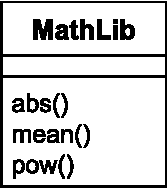
\includegraphics[width=\linewidth]{OriginalClassDiagram}
        \caption{origin}
        \label{fig:origin}
    \end{subfigure}
    \hfill
    \begin{subfigure}[t]{0.2\linewidth}
        \centering
        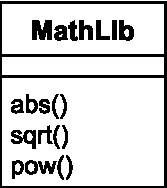
\includegraphics[width=\linewidth]{LeftClassDiagram}
        \caption{left}
        \label{fig:left}
    \end{subfigure}
    \hfill
    \begin{subfigure}[t]{0.2\linewidth}
        \centering
        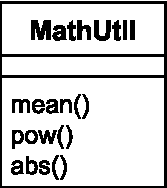
\includegraphics[width=\linewidth]{RightClassDiagram}
        \caption{right}
        \label{fig:right}
    \end{subfigure}
    \hfill
    \label{fig:versions}
    \caption{Different versions of a model.}
\end{figure}
\end{minipage}
\hfill
\begin{minipage}[t]{0.37\linewidth}
\begin{lstlisting}[style=eol,numbersep=0.6pt,caption={The pseudo-formatted CBP of the model in Fig. \ref{fig:origin}.},label=lst:origincbp]
create x type Class
set x.name to "Math" 
create a type Operation
set a.name to "abs" 
create b type Operation
set b.name to "mean" 
create c type Operation
set c.name to "pow" 
add a to x.operations at 0
add b to x.operations at 1
add c to x.operations at 2
\end{lstlisting}
\end{minipage}

  \vspace{-5pt}
\section{State-based Model Comparison}
\label{sec:model_comparison}

\vspace{-5pt}
In a collaborative modelling setting, a model can have different versions.
%\dk{Mutliple versions can exist even if a model is developed by a single developer}.
Consider the case where an initial version of a model exists in a Version Control System (VCS) server (Fig. \ref{fig:vcs}).
Two modellers, Bob and Alice, check out the original model (steps 1 and 2) to their local machines and modify it (steps 3 and 4).
Alice then commits her work (original + Alice's changes) to the VCS.
Since there is no newer commit on the VCS, the commit process is straightforward (step 5).
Bob then decides to also commit his work (original + Bob's changes) to the VCS.
However, he needs to merge his work with the current updated version at the VCS since his last checkout.
His machine downloads the latest version from the server (step 6), i.e. Alice's version.
To merge his and Alice's changes, Bob needs to perform model comparison to check their differences, resolve possible conflicts between the models, and then merge them (step 7).
After that, he can push it back to the VCS server.

\begin{figure}[ht]
    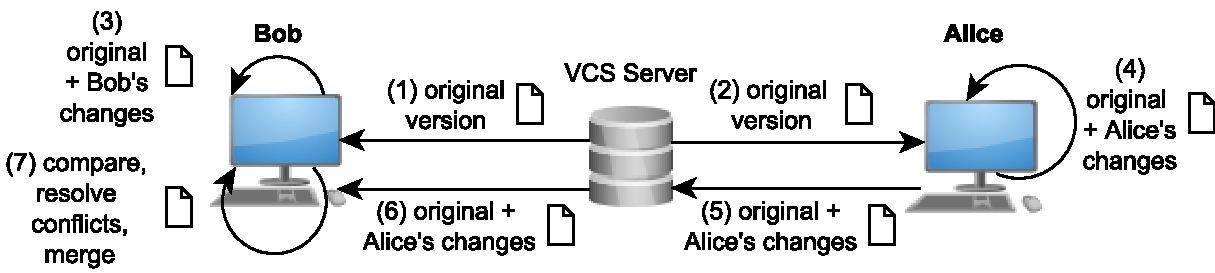
\includegraphics[width=\linewidth]{VCS}
    \caption{A usecase of CBP in a collaborative modelling.}
    \label{fig:vcs}
\end{figure}


In a SBP setting, Bob produces the model in Fig. \ref{fig:left} (the left model), and Alice the model in Fig. \ref{fig:right} (the right model) producing XMI files as shown in List. \ref{lst:leftxmi} and List. \ref{lst:rightxmi} respectively.
Before Bob can merge, he must compare the right model with the left model.
In state-based comparison, comparing models commonly consists of two steps: \emph{matching} and \emph{diffing}.
The matching process establishes matches between the elements of both models, to determine the elements in the left model that correspond to elements in the right model.
Generally, the matching process iterates through all the elements of the models being compared and matches them by their identifiers or through a similarity mechanism  \cite{DBLP:conf/sfm/BroschKLSWW12,emfcompare2018developer}.
%Note that for new and deleted elements the result of the match can be that there is no match.

The diffing process identifies differences between the matched elements \cite{DBLP:conf/sfm/BroschKLSWW12,emfcompare2018developer}.Differences between the matched elements and all their features is usually done using a Longest Common Subsequence (LCS) algorithm, e.g., \cite{DBLP:journals/algorithmica/Meyers86}.

\vspace{-10pt}
\begin{minipage}[t]{0.49\linewidth} 
    \begin{lstlisting}[style=eol,caption={The simplified XMI of the left model in Fig. \ref{fig:left}.},label=lst:leftxmi]
    <uml:Class id="x" name="MathLib">
    <operation id="a" name="abs/>
    <operation id="d" name="sqrt"/>
    <operation id="c" name="pow"/>
    </uml:Class>
    \end{lstlisting}
\end{minipage}
\hfill
\begin{minipage}[t]{0.49\linewidth}
    \begin{lstlisting}[style=eol,caption={The simplified XMI of the right model in Fig. \ref{fig:right}.},label=lst:rightxmi]
    <uml:Class id="x" name="MathUtil">
    <operation id="b" name="mean"/>
    <operation id="c" name="pow"/>
    <operation id="a" name="abs"/>
    </uml:Class>
    \end{lstlisting}
\end{minipage}

In our example, the matching process in state-based comparison -- as performed by EMF Compare \cite{emfcompare2018developer} -- iterates through all the elements of both models and matches them using their identifiers. The matching process yields 3 matches: $m_1$ = (\textsf{x}, \textsf{x}), $m_2$ = (\textsf{a}, \textsf{a}), and $m_3$ = (\textsf{c}, \textsf{c}), and 2 unmatched elements, $um_1$ = (\textsf{d}, -) and $um_2$ = (-, \textsf{b}). 

The diffing process then iterates through all the matches and unmatched elements and uses an LCS algorithm to identify their differences. In the first match, it identifies that the elements \textsf{x} are different in their \textsf{name} and \textsf{operations} features. The left \textsf{x}'s \textsf{name} is ``MathLib'' while the other \textsf{x}'s \textsf{name} is ``MathUtil'' (diff $ds_1$). The \textsf{operations} features are different in their contents -- the left \textsf{operations} feature does not contain element \textsf{b} (diff $ds_2$), the left \textsf{operations} feature contains element \textsf{d} that does not exist in the right \textsf{operations} (diff $ds_3$), and the indexes of element \textsf{c} are different in both features (diff $ds_4$). It is important to note that the employed LCS algorithm does not detect the different position of element \textsf{A} as a difference; it only identifies the minimum number of differences which if all are resolved unidirectionally can make both models equal. Otherwise, the number becomes less optimal -- not minimum.

Differences are commonly expressed as a list of changes that must be applied to a target model so that it is made equal to a reference model.
%\dk{We should probably consider different terminology here as the terms ``source'' and ``reference'' are very similar}.
This paper treats the left model as a reference model and the right model as the target model.
This means that differences are expressed as changes applied to the right model so that it equals the left model.
To express differences, we use the following terms: \textsf{LeftContainer}, \textsf{RightContainer}, \textsf{LeftFeature}, \textsf{RightFeature}, \textsf{LeftIndex}, \textsf{RightIndex}, \textsf{LeftValue}, \textsf{RightValue}, and \textsf{Kind}. The \textsf{*Container}, \textsf{*Feature}, and \textsf{*Value} are the target element, feature, and value involved in a difference (\textsf{*} symbol can be replaced with \textsf{Left} and \textsf{Right}). \textsf{*Index} is the index of a value in a feature. \textsf{Kind} is the type of difference. It can be one of these types: \textsf{CHANGE}, \textsf{ADD}, \textsf{DELETE}, and \textsf{MOVE}. \textsf{CHANGE} means a pair of single-valued features 
%features -- single-valued attributes or non-containment references \dk{Why is containment important?} -- 
have different values. \textsf{ADD} indicates that a value does not exist in the right model, thus it requires the addition of the value. \textsf{DELETE} is the opposite
%\dk{``opposite''?} 
of \textsf{ADD}. \textsf{MOVE} indicates that matched elements differ in terms of their containers, containing features, or indexes.
A Container is an element that contains a value. A containing feature is a feature owned by a container in which a value is contained. An index is the position of a value in a containing feature.

Based on these definitions, we can express the result of the diffing process as: $ds_{n}$ = [$LeftContainer_n$, $RightContainer_n$, $LeftFeature_n$, $RightFeature_n$, $LeftIndex_n$, $RightIndex_n$, $LeftValue_n$, $RightValue_n$, $Kind_n$]. Thus, $ds_{1}$ =  [\textsf{x}, \textsf{x}, \textsf{name}, \textsf{name}, 0, 0, ``MathLib'', ``Mathutil'', \textsf{CHANGE}], $ds_{2}$ = [\textsf{x}, \textsf{x}, \textsf{operations}, \textsf{operations}, null, 0, null, \textsf{b}, \textsf{DELETE}], $ds_{3}$ = [\textsf{x}, \textsf{x}, \textsf{operations}, \textsf{operations}, 1, null, \textsf{d}, null, \textsf{ADD}], and $ds_{4}$ = [\textsf{x}, \textsf{x}, \textsf{operations}, \textsf{operations}, 2, 1, \textsf{c}, \textsf{c}, \textsf{MOVE}]. We can use this information to represent the differences visually as depicted in Fig. \ref{fig:xmi_comparison}. Applying these differences as changes to the right model will transform it into the left model.  

\begin{figure}
    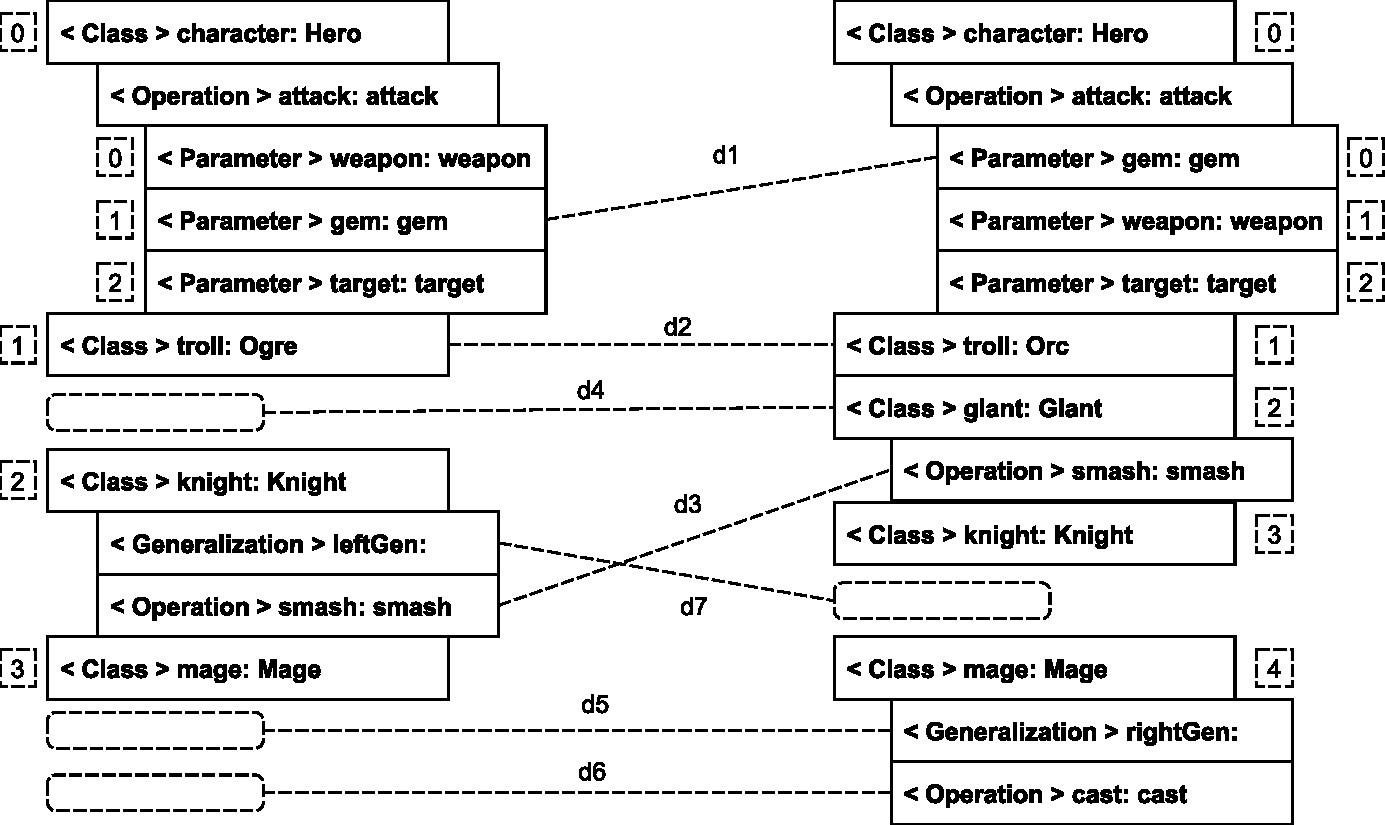
\includegraphics[width=\linewidth]{XmiComparison}
    \caption{A model comparison of the left and right models in Listings \ref{lst:leftxmi} and \ref{lst:rightxmi}.}
    \label{fig:xmi_comparison}
\end{figure}

\section{Change-based Approach for Comparing Models}
\label{sec:change_based_approach_for_comparing_models}

Now let's consider the same example in a CBP setting.
The changes made by Bob and Alice are appended to their local original CBP producing two different CBP representations as displayed in Listings \ref{lst:leftcbp} and \ref{lst:rightcbp}\footnote{Both CBPs only present the changes after the last line of the original version (start from line 12).} -- capturing different courses of modification made by the two modellers.
Then, the example is the same with Alice committing her changes and Bob wanting to merge Alice's work with his. 


\begin{minipage}[t]{0.49\linewidth}    
    \begin{lstlisting}[firstnumber=12,style=eol,caption={The appended changes made by Bob to produce the model in Fig. \ref{fig:left} (left version).},label=lst:leftcbp]
    set x.name from "Math" to "MathLib"
    create d type Operation
    set d.name to "sqrt"
    add d to x.operations at 1
    remove b in x.operations at 2
    delete b
    \end{lstlisting}
\end{minipage}
\hfill
\begin{minipage}[t]{0.49\linewidth}
    \begin{lstlisting}[firstnumber=12,style=eol,caption={The appended changes made by Alice to produce the model in Fig. \ref{fig:right} (right version).},label=lst:rightcbp]
    move a in x.operations from 0 to 2
    set x.name from "Math" to "MathUtil"
    \end{lstlisting}
\end{minipage}

%Since both modellers work using CBP, we can exploit the representation to improve the previous model comparison.
%For example, we do not need to visit, match, and differentiate both \textsf{c} elements in the running example as they are not affected by the recent changes in both CBPs; only the affected features by the recent changes to be compared -- not all features. 
In CBP, comparison has three phases: event loading, element tree construction, and diff computation.
Further, comparison is not performed over all the elements of the model; instead, we only need to compare the last set of changes from the source and reference model.
The last set of changes can be identified easily by finding their last common change.
A simplified class diagram of our approach's implementation\footnote{The source can be found at \url{https://github.com/epsilonlabs/emf-cbp}.} is depicted in Fig. \ref{fig:approach_class_diagram}. 
Next, we describe the three phases in detail.

\begin{figure}
    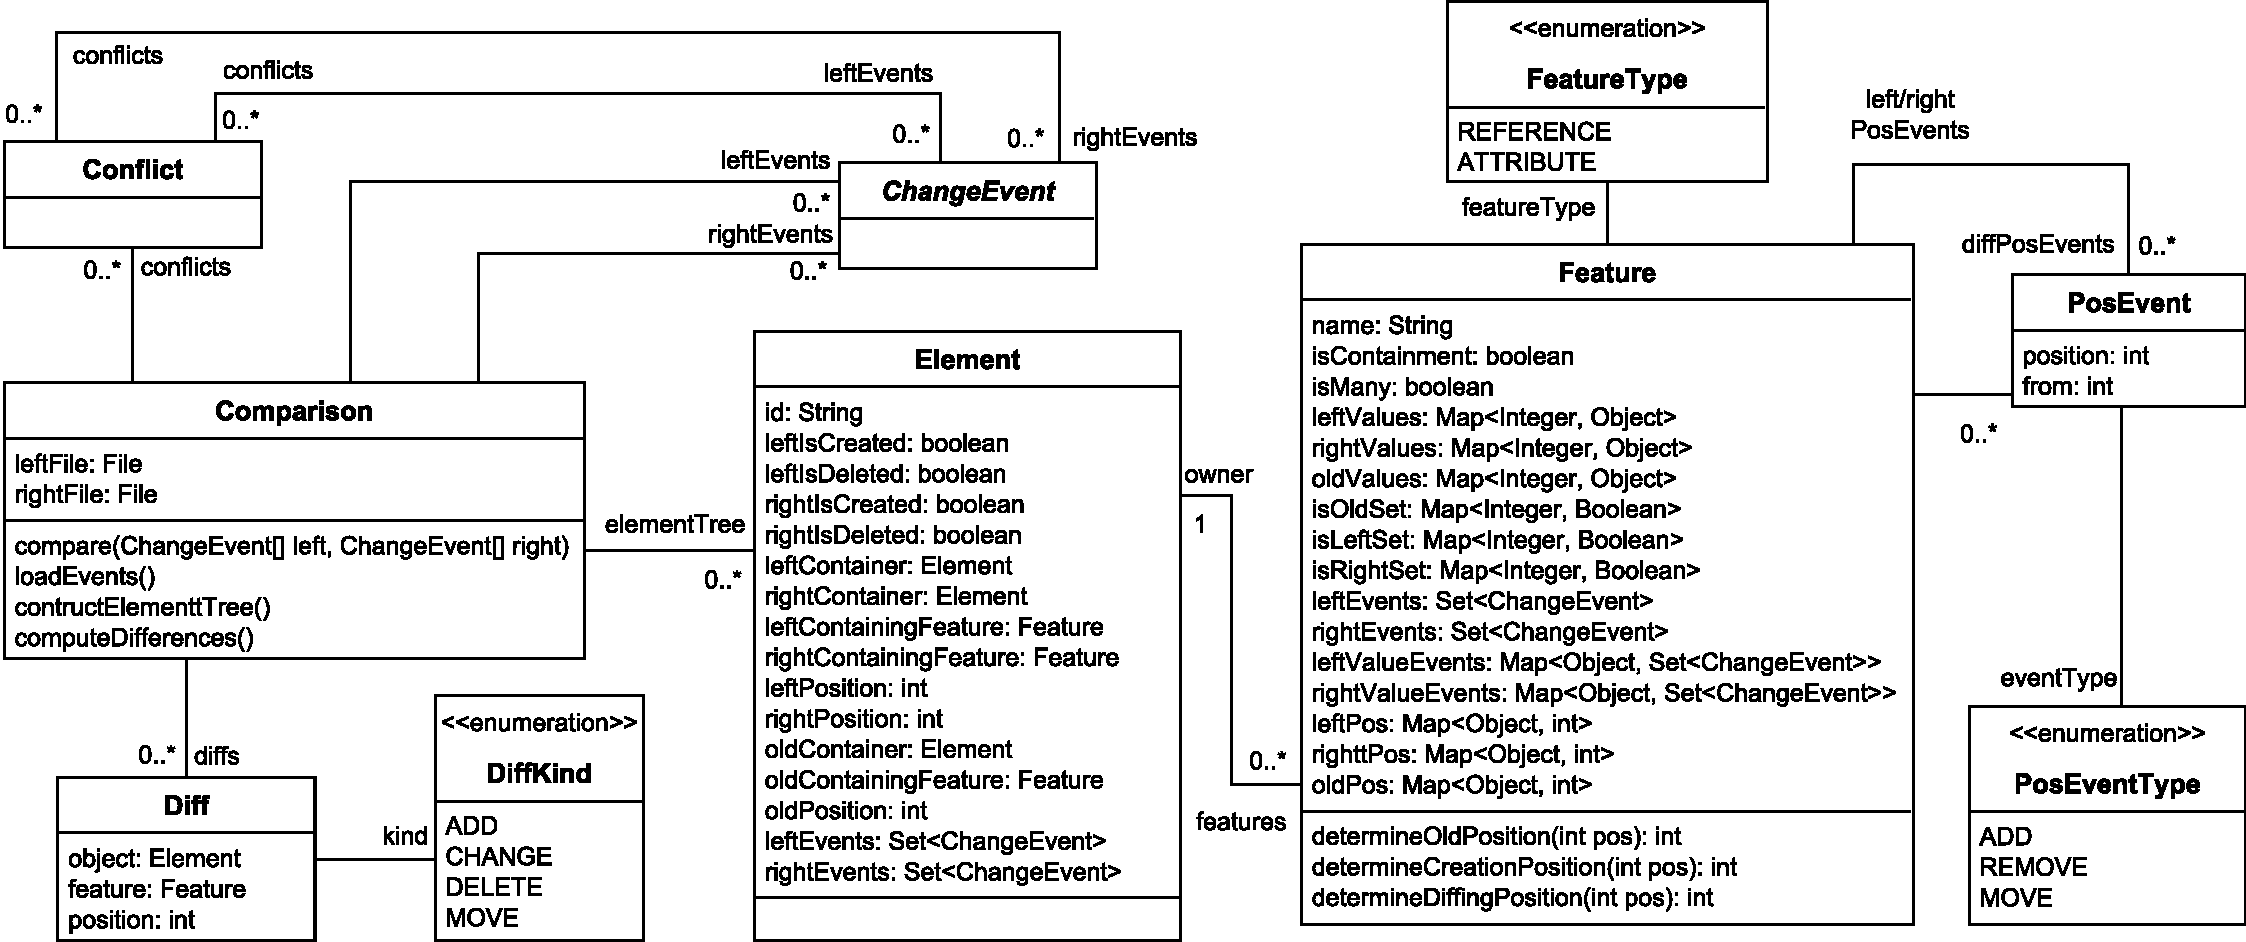
\includegraphics[width=\linewidth]{TreeClassDiagram}
    \caption{A class diagram showing the core components of the change-based approach to speed up model comparison.}
    \label{fig:approach_class_diagram}
\end{figure}


\subsection{Event Loading}
\label{sec:event_loading}
In the event loading phase, our implementation loads change events recorded in two CBP files into memory.
The most important aspect of this phase is the partial loading as only lines starting from the position where the two files are different are loaded.
Thus, not the whole model needs to be traversed and loaded.
In this case, lines 1-11 in List. \ref{lst:origincbp} are skipped.

Only lines starting from line 12 in Listings \ref{lst:leftcbp} and \ref{lst:rightcbp} are loaded, yielding two partial -- left and right -- change-event models. 

\begin{wrapfigure}[35]{r}{0.5\textwidth}
    \vspace{-30pt}
    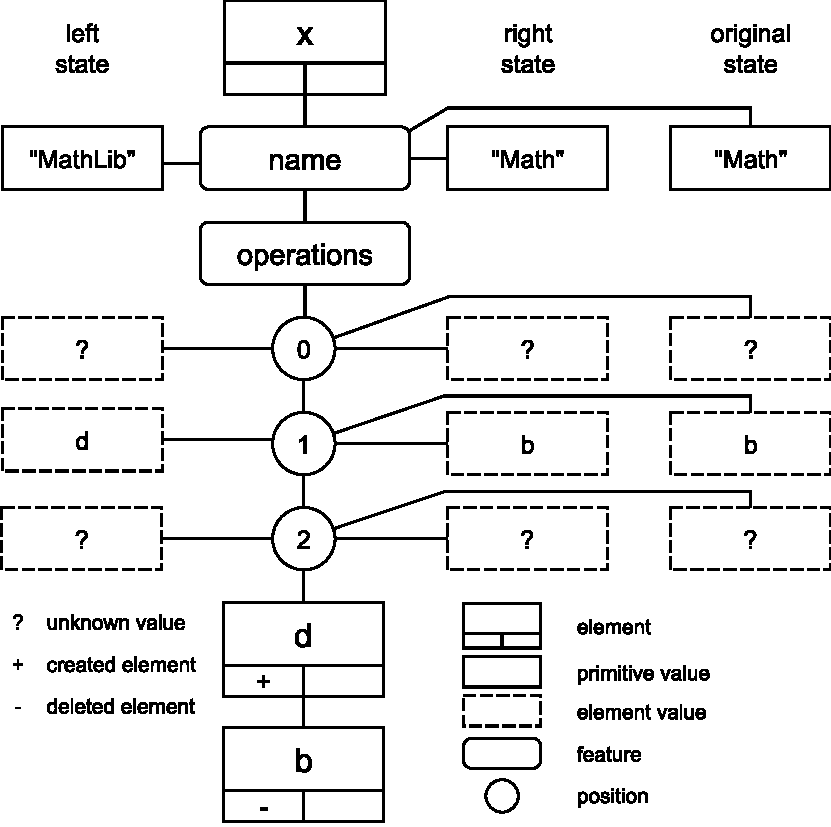
\includegraphics[width=\linewidth]{LeftElementTreeDiagram}
    \caption{The \textsf{elementTree} after processing all left change events.}
    \label{fig:left_element_tree_diagram}
    \vspace{1em}
    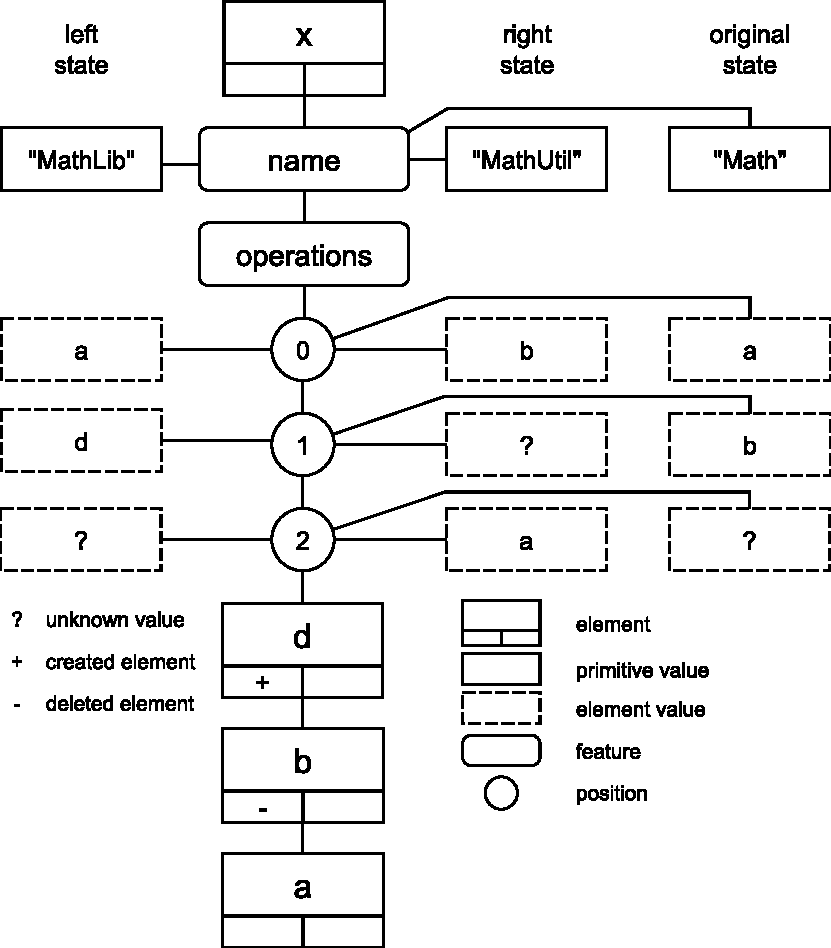
\includegraphics[width=\linewidth]{RightElementTreeDiagram}
    \caption{The \textsf{elementTree} after processing all left and right change events.}
    \label{fig:right_element_tree_diagram}
\end{wrapfigure}

\subsection{Element Tree}
\label{sec:tree_construction}
An element tree is a representation of the changes of model elements in the source and reference models. It contains detailed information about elements and their properties. It contains similar information to that captured in change lists in SBP, but also provides more information about the changes. For example, the element tree can keep track of a feature's old value and element/value's indexes inside multi-valued properties. The element tree only contains the partial states of affected elements of the original, left, and right models as depicted in Figures \ref{fig:left_element_tree_diagram} and \ref{fig:right_element_tree_diagram}.

To better understand the construction of an element tree from change events, we use the following running example using both change events in the Listings \ref{lst:leftcbp} and \ref{lst:rightcbp}. We start from the left change events. 

\subsubsection{Left Side}\label{sec:left_side}
%In List. \ref{lst:leftcbp}, 

From the first event [\texttt{\small \textbf{set} x.name \textbf{from} "Math" \textbf{to} "MathLib"}] at line 12, we can identify that an element with id \textsf{x} has existed from the original model. 
%\dk{Incomplete sentence?}
It has a feature \textsf{name} with a value ``Math'' in the original model that has been changed to ``MathLib'' in the left model. Since the element \textsf{x} does not already exist in the \textsf{elementTree}, we create its instance of \textsf{Element} and also its feature \textsf{name}. We set the value of the feature \textsf{name} to ``MathLib'' and also set it to ``Math'' in the partial state of the original model -- it has not been set before. As this feature on the right side also has not been set, we set it to ``Math'' as well. 
%Once a feature in the original state has been set, it cannot be overridden -- using the flag \textsf{isOldSet} in class \textsf{Feature} in Fig. \ref{fig:approach_class_diagram}. 

At line 13, in the event [\texttt{\small \textbf{create} d \textbf{type} Operation}], we can identify that an element with id \textsf{d} has been created. We also update the \textsf{elementTree} to include this element and set the element's flag \textsf{leftIsCreated} to \textsf{true}. In the event [\texttt{\small \textbf{set} d.name \textbf{to} "sqrt"}] at line 14, we can identify that element \textsf{d}'s feature \textsf{name} has been set to ``sqrt''. Thus, we update \textsf{d}'s feature \textsf{name} in the \textsf{elementTree}. From the event [\texttt{\small \textbf{add} d \textbf{to} x.operations \textbf{at} 1}] at line 15, we can deduce that element \textsf{d} is added to index 1 in the element \textsf{x}'s feature \textsf{operations}. Thus, we assign \textsf{d} to element \textsf{x}'s feature \textsf{operations} at index 1 in the \textsf{elementTree}. As \textsf{d} is a new element that only exists in the left model, we do not update changes of this element to the original and right models. 

From the event [\texttt{\small \textbf{remove} b \textbf{in} x.operations \textbf{at} 2}] at line 16, we can identify that there is element \textsf{b} in the original model, but it is deleted in the left model. The index of element \textsf{b} in the original model can be calculated back through the previous change events that have been applied to its feature. Since the previous event is adding element \textsf{d} to index 1 and the index of \textsf{b} is at 2 at the time it is removed, we can deduce that before element \textsf{d} is added, the index of element \textsf{b} is at 1 and is shifted to 2 because of the addition of element \textsf{d}.  Therefore, we can conclude that the original index of element \textsf{b} is at 1. Thus, we update the original state of the \textsf{elementTree} by adding element \textsf{b} into the element \textsf{x}'s feature \textsf{operations} at index 1.  

We perform the same procedure to also add element \textsf{b} to the right state of the \textsf{elementTree}. However, since no change event has been applied to the right side of element \textsf{x}'s feature \textsf{operations}, the calculation of element \textsf{b}'s index should return the same value as in the original state (line 13, Alg. \ref{alg:element_tree}), and thus element \textsf{b} has the same index as in the original state. It is important to notice, in this step, the flag \textsf{isRightSet} (class \textsf{Feature}, Fig. \ref{fig:approach_class_diagram}) is not set to \textsf{true} since we want the value to be able to be overridden during processing of the right change events. The last event [\texttt{\small \textbf{delete} b}], removes the element \textsf{b} from the left model. Hence, we set the flag \textsf{leftIsDeleted} of element \textsf{a} to \textsf{true}.

Fig. \ref{fig:left_element_tree_diagram} illustrates the state of the \textsf{elementTree} after all left change events have been processed. As can be seen, the \textsf{elementTree} exhibits the partial states of the original, left, and right models at once. 

\subsubsection{Right Side}\label{sec:right_side}  From the first event [\texttt{\small \textbf{move} a \textbf{in} x.operations \textbf{from} 0 \textbf{to} 2}] at line 12, we can infer that in the right model there is an element with id \textsf{a} positioned at index 2 in the element \textsf{x}'s feature \textsf{operations}. Thus, element \textsf{a} -- an instance of class \textsf{Element} in \ref{fig:approach_class_diagram} -- is added to the \textsf{elementTree} and positioned at index 2 of the element \textsf{x}'s feature \textsf{operations}. Since the event is a \textsf{move} type and the new index is larger than its previous index, elements that are between its previous and new indexes are shifted one place down. As element \textsf{b} has already existed in the same feature (the element was added during the process of the left change events) and its index is between element \textsf{a}'s movement, the index of element \textsf{b} is shifted down from 1 to 0. 

Also, since the event's type is \textsf{move} and its previous index is 0 and it is the first event that changes the index of element \textsf{a}, these conditions imply that element \textsf{a} in the original model is positioned at index 0 in the element \textsf{x}'s feature \textsf{operations}. Therefore, we add the element \textsf{a} to element \textsf{x}'s feature \textsf{operations} in the original state of the \textsf{elementTree}. Since the index 0 in the element \textsf{x}'s feature \textsf{operations} has not been set, we also add element \textsf{a} to that index in the right state of the \textsf{elementTree}. From the last event [\texttt{\small \textbf{set} a.name \textbf{from} "Math" \textbf{to} "MathUtil"}] at line 13, we can infer that in the right model, the value of element \textsf{a}'s feature \textsf{name} is ``MathUtil''. Hence, we set the feature \textsf{name} to ``MathUtil'' in the right state. 
We do not apply this operation to the original and left states as they have been set before.
Fig. \ref{fig:right_element_tree_diagram} exhibits the state of the \textsf{elementTree} after both sides' change events have been processed.

\begin{figure}
    \centering
    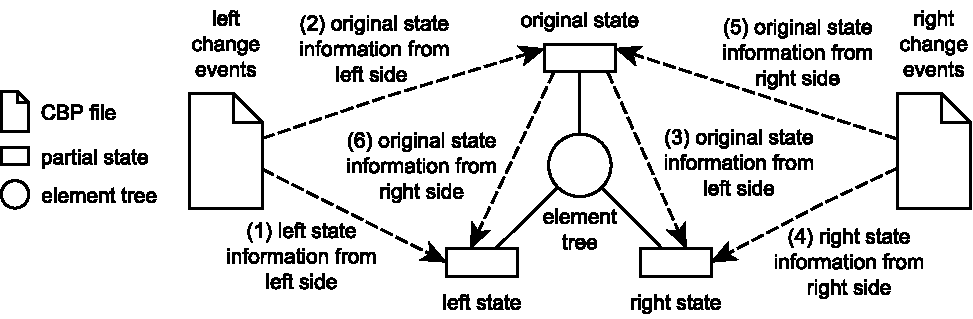
\includegraphics[width=0.7\linewidth]{TreeConstruction}
    \caption{Steps in Element Tree construction.}
    \label{fig:tree_construction}
\end{figure} 

The construction of the \textsf{elementTree} that we have just explained follows the steps shown in Fig. \ref{fig:tree_construction}. First, the partial
%left \dk{Delete ``left''?} 
state $S_{L}$ of the left model in the \textsf{elementTree} is constructed based on the information retrieved from the left change events (step 1). We denote this information as $I_{LL}$. We can also construct the partial 
%original \dk{Delete ``original''?} 
state $S_{O}$ of the original model using the information related to the original state contained in the left change events $I_{OL}$ (step 2). The information $I_{OL}$ allows us to construct the initial partial 
%right \dk{Delete ``right''?} 
state $S_{R}$ of the right model 
%before updated \dk{This doesn't read well} by the right change events 
(step 3). Similarly, using the information from the right change events $I_{RR}$, we update the partial right state $S_{R}$ that has been initialised before using the information $I_{OL}$ (step 4), implying that $I_{OL} \cup I_{RR} \rightarrow S_{R}$. Also, information related to the state of the original model from the right change events $I_{OR}$ is used to update the original state  (step 5). Thus, we have a partial state of the original model constructed using information from both left and right sides, $I_{OL} \cup I_{OR} \rightarrow S_{O}$. Finally, we also use the information $I_{OR}$ to update the partial state of the left model (step 6), implying that $I_{LL} \cup I_{OR} \rightarrow S_{L}$.  

Alg. \ref{alg:element_tree} describes the steps presented in Fig. \ref{fig:tree_construction} in a generic fashion. It iterates through all of a model's change events and uses the information contained in them to construct the relevant partial state. The selection of side, left or right change events, that are executed first depends on the \textsf{Side} enumeration value -- \textsf{left} or \textsf{right} -- passed through the parameter \textsf{side} (the second input parameter). In our implementation, we process the left side first by default. The algorithm also receives an input of the change events \textsf{events} that are to be iterated and the element tree \textsf{elementTree} that has been instantiated before, and then returns the \textsf{elementTree} as output after updating it.

For each \textsf{event} in the \textsf{events}, we collect information needed to build up the \textsf{elementTree}  (lines 3-9), such as \textsf{targetElement}, \textsf{feature}, \textsf{value}, \textsf{previousValue}, \textsf{index}, and \textsf{previousIndex}. The \textsf{targetElement} is the element modified by a change event (e.g., \textsf{x} and \textsf{d} in List. \ref{lst:leftcbp}). This \textsf{targetElement} -- an instance of class Element in Fig. \ref{fig:approach_class_diagram} -- is retrieved from the \textsf{elementTree} if it already exists. Otherwise, a new element is created and added to the \textsf{elementTree} (line 3). In this step we also set the flags \textsf{*IsCreated} and \textsf{*IsDeleted} of the element in Fig. \ref{fig:approach_class_diagram}. For example, if the type of the event is \textsf{create} then \textsf{*IsCreated} is set to \textsf{true}. The \textsf{feature} -- an instance of class Feature in Fig. \ref{fig:approach_class_diagram} -- represents the target element's feature (e.g., \textsf{name} and \textsf{operations} in List. \ref{lst:leftcbp}) modified by a change event. It is retrieved from the \textsf{targetElement}'s feature list, and a new one is created and added to the \textsf{targetElement}'s feature list if the feature does exist (line 5). 

The \textsf{value} is the value assigned to the feature in a change event (line 5, Alg. \ref{alg:element_tree}). The \textsf{value} can be the type of \textsf{Element} (e.g., elements \textsf{b} and  \textsf{d}, lines 17-18, List. \ref{lst:leftcbp}) or primitive (e.g., the string ``MathLib'' at line 14 in the List. \ref{lst:leftcbp}). The \textsf{previousValue} represents the previous value of the modified feature (line 6, Alg. \ref{alg:element_tree}). The \textsf{previousValue} is not defined if no previous value has been assigned. For \textsf{value} and \textsf{previousValue} with type \textsf{Element}, the elements that they represent are retrieved from the \textsf{elementTree}, and if they do not exist, new instances are created. If the type is primitive, the value is treated as it is. Not every change event has a \textsf{value}, particularly events with type \textsf{create} 
%\dk{Should this be ``create'' instead?} 
or \textsf{delete} which only modify a target element not the element's feature.

\IncMargin{1.5em}
\begin{algorithm}[H]
    \begin{footnotesize}
        \SetKwInOut{Input}{input} 
        \SetKwInOut{Output}{output}
        \Input{a list of ChangeEvent $events$}
        \Input{an enumeration of Side $side$}
        \Input{an instance of ElementTree $elementTree$}
        \Output{an instance of ElementTree $elementTree$}
        \SetKwBlock{Beginn}{beginn}{ende}
        \Begin{
            \ForEach{$event$ in $events$}{
                $targetElement$ $\leftarrow$ getOrCreateNewTargetElement($event$, $elementTree$)\;
                $feature$ $\leftarrow$ getOrCreateNewFeature($event$, $targetElement$)\;
                $value$ $\leftarrow$ getValue($event$)\;
                $previousValue$ $\leftarrow$ getPreviousValue($event$)\;
                $index$ $\leftarrow$ getIndex($event$)\;
                $previousIndex$ $\leftarrow$ getPreviousIndex($event$)\;
                $featureEventList$ $\leftarrow$ getFeatureEventList($feature$, $side$)\;
                
                \BlankLine
                \tcp{put all values to their proper indexes}
                updateTree($targetElement$, $feature$, $value$, $index$, $side$)\;
                $oldIndexes$ $\leftarrow$ calculateOldIndex($featureEventList$, $previousIndex$, $side$)\;
                \If{\Not isCreated($value$, $side$) \AndA \Not isOldValueSet($feature$, $previousValue$, $previousIndex$, $side$)} {
                    setOldValue($feature$, $previousValue$, $oldIndex$, $side$)\;
                    $oppositeFeatureEventList$ $\leftarrow$ getOppositeFeatureEventList($feature$, $side$)\;
                    $oppositeIndex$ $\leftarrow$ calculateOppositeIndex($oppositeFeatureEventList$, $oldIndex$, $side$)\;
                    \If{\Not isDeleted($value$, $side$) \AndA \Not isOppositeSideValueSet($feature$, $value$, $oppositeIndex$, $side$)} {
                        setOppositeSideValue($feature$, $value$, $oppositeIndex$, $side$)\;
                    }
                }   
                
                addEventToFeatureEventList($event$, $featureEventList$)\;
                
            }
            \Return{$elementTree$}\;
        }
    \end{footnotesize}
    \caption{Algorithm to construct an element tree from events.}
    \label{alg:element_tree}
\end{algorithm}
\DecMargin{1.5em}

 
The \textsf{index} is the index assigned by a change event to a value in a feature, while \textsf{previousIndex} is the previous index of the value (lines 7-8, Alg. \ref{alg:element_tree}). In one change event, we can get both \textsf{index} and \textsf{previousIndex} or only one of them depending on the type of the change event. For example, we can only obtain that the \textsf{index} of \textsf{d} is 1 (line 17 in List. \ref{lst:leftcbp}) as the change event type is \textsf{add}. In a \textsf{remove} change event, we can only get the \textsf{previousIndex} of \textsf{b}, that is 2 (line 17 in List. \ref{lst:leftcbp}), as the element does not exist anymore in the left model. We can obtain both of them only in a \textsf{move} change event as an element is moved from a previous index to a new one (line 14 in List. \ref{lst:rightcbp}). For a single-valued feature, the \textsf{index} and \textsf{previousIndex} are always 0 as the feature can only contain a single value. 

At line 9, we retrieve the \textsf{featureEventList} from the \textsf{feature} to be added later with the current \textsf{event} (line 19). The \textsf{featureEventList} is a list -- a history -- of change events that have been processed that are specific to the \textsf{feature} on the selected \textsf{side}. Using the obtained \textsf{targetElement}, \textsf{feature}, \textsf{value}, and \textsf{index}, the process then updates the state of the \textsf{elementTree} on the selected \textsf{side} (line 10). After that, it calculates back the original index of a value using the \textsf{featureEventList} and \textsf{previousIndex} (line 11). If the value at \textsf{oldIndex} in the \textsf{feature} has not been set, then the algorithm sets the \textsf{feature} with the \textsf{previousValue} at the \textsf{oldIndex} in the partial state of the original model (lines 12-13). At lines 14-18, the algorithm also does the same thing to the opposite side -- if the current \textsf{side} is \textsf{left} then it is \textsf{right}.  

\subsection{Diff Computation}
\label{sec:diff_computation}

Using the \textsf{elementTree} presented in Fig. \ref{fig:right_element_tree_diagram}, we can determine the difference between the left and right models without having to compare all their elements and features. After the \textsf{elementTree} has been constructed, we iterate through elements and features of the \textsf{elementTree} and use the flags, containers, containing features, and indexes on both sides of each element and value to identify differences between both left and right models. We follow the steps in Alg. \ref{alg:diff_calculation}. The algorithm visits each element and every index of each feature (lines 3-5). At every index, it retrieves the \textsf{leftValue} and \textsf{rightValue} (lines 5-7), passing these, together with the \textsf{element}, \textsf{feature}, and \textsf{index} to a function \textsf{identifyDiffUsingRules} (line 8). The function identifies differences using a set of pre-defined rules which determines differences \textsf{diffs} based on the states of flags of an element, flags and attributes of the element's feature, values of the feature, and indexes of the values. The obtained \textsf{diffs} are then added to the overall list of differences \textsf{diffList} which is output (line 8-9, 13). 

\IncMargin{1.5em}
\begin{algorithm}[H]
    \begin{footnotesize}
        \SetKwInOut{Input}{input}
        \SetKwInOut{Output}{output}
        \Input{an instance of ElementTree $elementTree$}
        \Begin{
            $diffList$ $\leftarrow$  DiffList()\;
            \ForEach{$element$ \In $elementTree$}{
                \ForEach{$feature$ \In getFeatures($element$)}{
                    \ForEach{$index$ \In getIndexes($feature$)}{
                        $leftValue$ $\leftarrow$ getLeftValue($feature$, $index$)\;
                        $rightValue$ $\leftarrow$ getRightValue($feature$, $index$)\;
                        \BlankLine
                        \tcp{rules starts from here}
                        $diffs$ $\leftarrow$ identifyDiffUsingRules($element$, $feature$, $leftValue$, $rightValue$, $index$)\;
                        addToDiffList($diffs$,$diffList$)\;
                    }
                }
            }
            \Return{$diffList$}\;
        }
    \end{footnotesize}
    \caption{Algorithm to determine differences.}
    \label{alg:diff_calculation}
\end{algorithm}
\DecMargin{1.5em}

We illustrate the principles and use of rules by discussing the rules used to identify differences in the running example, which can be found in Alg. \ref{alg:diff_rules}. The algorithm is the breakdown of the function \textsf{identifyDiffUsingRules} in Alg. \ref{alg:diff_calculation}. As previously stated, it is important to remember that we use the left model as a reference which means the differences are presented as changes that transform the right model to become equal to the left model. 

The first rule (Rule 1) in Alg. \ref{alg:diff_rules} is to identify changes in single-valued attributes. A feature has to be of type \textsf{attribute}, both side values have to be different, and the element should have not been created or deleted in both models. The second rule (Rule 2) identifies whether an element is in a different location in both models. The element must not have been deleted and must exist from the previous version -- the original model. Also, its containers, containing features, or indexes of the element have to be different on both sides.

\IncMargin{1.5em}
\begin{algorithm}[H]
    \begin{footnotesize}
        \SetKwInOut{Input}{input}
        \SetKwInOut{Output}{output}
        \Input{an Element $element$, a Feature $feature$, a variable $leftValue$, a variable $rightValue$, an Integer $index$}
        \Output{a List of Diff $diffs$}
        $diffs$ $\leftarrow$ createDiffList()\;
        \tcp{...}
        \tcp{Rule 1: a rule to determine a change of a single-valued attribute}
        \If{getType($feature$) \Is Attribute \AndA isSingleValued($feature$) \AndA leftValue <> rightValue \AndA \Not leftIsCreated($element$) \AndA \Not leftIsDeleted($element$) \AndA \Not  rightIsCreated($element$) \AndA \Not rightIsDeleted($element$)}{
            $diff$ $\leftarrow$ createNewDiff($element$, $element$, $feature$, $feature$, $index$, $index$, $leftValue$, $rightValue$, DifferenceType.CHANGE)\;
            addDiffToDiffList($diff$, $diffs$)\;
        } 
        \tcp{Rule 2: one of rules to determine movement of an element}
        \If{getType($feature$) \Is Containment \AndA \Not leftIsCreated($leftValue$) \AndA \Not leftIsDeleted($leftValue$) \AndA \Not rightIsCreated($leftValue$) \AndA \Not rightIsDeleted($leftValue$) \AndA (getLeftContainer($leftValue$) <> getRightContainer($leftValue$) \Or getLeftFeature($leftValue$) <> getRightFeature($leftValue$) \Or getLeftIndex($leftValue$) <> getRightIndex($leftValue$))}{
            $diff$ $\leftarrow$ createNewDiff(getLeftContainer($leftValue$), getRightContainer($leftValue$), getLeftFeature($leftValue$), getRightFeature($leftValue$), getLeftIndex($leftValue$), getRightIndex($leftValue$), leftValue, leftValue, DifferenceType.MOVE)\;
            addDiffToDiffList($diff$, $diffs$)\;
        }
        \tcp{Rule 3: one of rules to determine deletion of an element}
        \If{getType($feature$) \Is Containment \AndA \Not leftIsCreated($rightValue$) \AndA leftIsDeleted($rightValue$) \AndA \Not rightIsCreated($rightValue$) \AndA \Not rightIsDeleted($rightValue$) }{
            createNewDiff(getLeftContainer($rightValue$), getRightContainer($rightValue$), getLeftFeature($rightValue$), getRightFeature($rightValue$), getLeftIndex($rightValue$), getRightIndex(), rightValue, null, DifferenceType.DELETE)\;
            addDiffToDiffList($diff$, $diffs$)\;
        }
        \tcp{Rule 4: one of rules to determine addition of an element}
        \If{getType($feature$) \Is Containment \AndA leftIsCreated($leftValue$)  \AndA \Not leftIsDeleted($leftValue$) \AndA \Not rightIsCreated($leftValue$) \AndA \Not rightIsDeleted($leftValue$)}{
            $diff$ $\leftarrow$ createNewDiff(getLeftContainer($leftValue$), getRightContainer($leftValue$), getLeftFeature($leftValue$), getRightFeature($leftValue$), getLeftIndex($leftValue$), getRightIndex($leftValue$), null, rightValue, DifferenceType.ADD)\;
            addDiffToDiffList($diff$, $diffs$)\;
        }
        \tcp{...}
        \Return{$diffs$}
    \end{footnotesize}
    \caption{Some rules to determine differences.}
    \label{alg:diff_rules}
\end{algorithm}
\DecMargin{1.5em}

The third rule (Rule 3) identifies the deletion of an element. If an element in the left model is not created but exists in the model, it means that the element has been there from the previous version -- the original model. This also means that the element also exists in the right model, unless it has been deleted. Thus, in order to make the right model equal to the left model, the element has to be deleted also in the right model. The fourth rule (Rule 4) identifies the need for an addition of an element. If an element is created in the left model and has not been deleted, it means that the element should be added also to the right model to make both models equal.

In the running example, when the iteration of the \textsf{elementTree} (Fig. \ref{fig:right_element_tree_diagram}) returns feature \textsf{name}, the type of the feature is a single-valued attribute and both sides of the feature are different in their values, this means that the condition of the first rule is met. Thus, we can conclude that in order to make the left value of the feature equal to the right value, we must override the value ``MathUtil'' with ``MathLib''; the type of this difference is \textsf{CHANGE}. When the iteration is at index 0 in the element \textsf{x}'s feature \textsf{operations}, we have two values: the \textsf{leftValue} is element \textsf{a}, and the \textsf{rightValue} is element \textsf{b}. As \textsf{a} exists
%As \textsf{a} exists \dk{Change to ``As a exists''?} 
on both sides -- all \textsf{*Created} and \textsf{*Deleted} flags are false, and it also has a different index, at 0 in the left state and 2 in the right state. This meets the condition of the second rule. Thus, we can conclude that in order to make the index of element \textsf{a} in the right model equal its index in the left model, element \textsf{a} should be moved from index 2 to 0. Thus, the type of this difference is \textsf{MOVE}. 

Element \textsf{b} used to exist but has been deleted from the left model (flags \textsf{leftIsCreated} = false, \textsf{leftIsDeleted} = true); it still exists in the right state (flags \textsf{rightIsCreated} = false, \textsf{rightIsDeleted} = false). This condition satisfies the third rule. Therefore, the element \textsf{b} should be deleted from the right model; the type of this difference is \textsf{DELETE}. We can get only one value when the iteration is at index 1 in the element \textsf{x}'s feature \textsf{operations}; the \textsf{leftValue} is element \textsf{d}, but the \textsf{rightValue} is unidentified. Thus, we only process the \textsf{leftValue}. Element \textsf{d} is only created in the left model (flags \textsf{leftIsCreated} = true, \textsf{leftIsDeleted} = false, \textsf{rightIsCreated} = false, \textsf{rightIsDeleted} = false). This meets the condition of the fourth rule. Thus, to make element \textsf{d} also exist in the right state, we must add it into element \textsf{x}'s feature \textsf{operations} at index 1. Therefore, the type of this difference is \textsf{ADD}. At index 2, the element \textsf{a} is skipped because it has been processed already. 

Similar to the state-based approach in Section \ref{sec:model_comparison}, we express identified differences as $dc_{n}$ = [$LeftContainer_n$, $RightContainer_n$, $LeftFeature_n$, $RightFeature_n$, $LeftIndex_n$, $RightIndex_n$, $LeftValue_n$, $RightValue_n$, $Kind_n$]. Thus, $dc_{1}$ =  [\textsf{x}, \textsf{x}, \textsf{name}, \textsf{name}, 0, 0, ``MathLib'', ``Mathutil'', \textsf{CHANGE}], $dc_{2}$ = [\textsf{x}, \textsf{x}, \textsf{operations}, \textsf{operations}, ?, 0, ?, \textsf{b}, \textsf{DELETE}], $dc_{3}$ = [\textsf{x}, \textsf{x}, \textsf{operations}, \textsf{operations}, 1, ?, \textsf{d}, ?, \textsf{ADD}], and $dc_{4}$ = [\textsf{x}, \textsf{x}, \textsf{operations}, \textsf{operations}, 0, 2, \textsf{a}, \textsf{a}, \textsf{MOVE}]. This change-based approach might produce differences that are distinct from differences identified using state-based approach. This can be seen between by comparing $ds_{4}$ and $dc_{4}$ ($ds_{4}$ $\neq$ $dc_{4}$, [\textsf{x}, \textsf{x}, \textsf{operations}, \textsf{operations}, 2, 1, \textsf{c}, \textsf{c}, \textsf{MOVE}] $\neq$ [\textsf{x}, \textsf{x}, \textsf{operations}, \textsf{operations}, 0, 2, \textsf{a}, \textsf{a}, \textsf{MOVE}]). In the state-based approach, element \textsf{c} has a \textsf{MOVE} difference -- it has different index ($ds_{4}$), while in the change-based approach, this difference is attributed to element \textsf{a} ($dc_{4}$). However, in both approaches, if we resolve their differences by performing all-left-to-right merging  -- making the right model equal to the left model, both approaches produce two models that are equivalent. In this way, we can check the correctness of the identified differences produced by the change-based approach.

\vspace{-10pt}
\section{Evaluation}
\label{sec:evaluation}
In this section, we present the method that we employed to evaluate our change-based comparison approach and discuss the results. We also present the limitations and threats to the validity of the evaluation.
\subsection{Method}
\label{sec:method}
In order to assess the performance benefits of the change-based approach in terms of model comparison, we have evaluated it against a mature and widely-used state-based comparison tool (EMF Compare \cite{emfcompare2018developer,eclipse2017compare}). Since there are no manually developed, large models persisted in our change-based format yet, the dataset for our experiments was constructed from a large model reverse-engineered from the Eclipse Epsilon project \cite{eclipse2018epsilongit,eclipse2017epsilon}. This model conforms to the Java metamodel \cite{eclipse2018modiscojava} and consists of more than 1.6 million elements with a size of 224 MBs when persisted in XMI. 

We cloned the original model to produce two new (left and right) models and perform operations (\textsf{add}, \textsf{remove}, \textsf{move}, \textsf{set} with random elements, features, indexes, and values) on both models to create differences. We made 1.1 million artificial changes to each model, generating over 1.1 million events (one operation can generate more than one event, e.g., a \textsf{move} between features generates \textsf{remove} and \textsf{add} events). Events generated by the changes were persisted in our change-based format (to be used later in change-based model comparison). After every 50,000 changes, we made a measurement point. We persisted the last state of the models in state-based format (to be used later in state-based model comparison) and then performed change-based and state-based model comparison and measured their execution time and memory footprint. We created 22 measurement points to capture their trends in one experiment. 

We conducted five experiments.
%batches \dk{Would it make sense to call these ``experiments'' instead? i.e. ``We conducted five experiments. In the first experiment \ldots''}. 
In the first experiment, the ratio of occurrence between \textsf{add}, \textsf{remove}, \textsf{move}, and \textsf{set} changes is set to 1:1:20:40 intuitively in assumption that in a mature model modification -- \textsf{move} and \textsf{set} events -- occurs more frequent than addition and deletion. Since we wanted the change of total elements not to affect our measurement, the number of total elements should be kept constant. For example, it is difficult to tell an increase of time in comparison is caused by an increase in the number of elements or by the number of change events. One way to do this was to exclude \textsf{add} and \textsf{remove} operations. However, excluding both operations made measurement less representative. Thus, we still included both operations but made their probabilities equal so that the number of total elements remain largely unchanged. In the rest of the experiments,
%batches \dk{Replace with ``In the remaining four experiments''? - it may not be entirely clear to the reviewers what ``to support'' means in this context}
we only performed homogeneous type operations -- isolated from other types -- per experiment (e.g., add-only, move-only operations). In the end, we obtained 5 results of the experiments: mixed, add-only, remove-only, move-only, and set-only measurement results. We did this to asses whether operations of different types have a different impact on model comparison.
%\dk{Explain that we did this to assess whether events of different types have a different impact on model comparison?}

For the change-based approach, the comparison time comprises loading change events, constructing an element tree, and identifying differences. The memory footprint is the space used to hold the change events, element tree, and differences in memory. For the state-based approach, the comparison time comprises matching elements and identifying differences, and the memory footprint is the space required to hold the matches and differences in memory. All measurements were performed on the same machine with the following specification: AMD Opteron(tm) Processor 6386 SE @ 2.8 GHz cache size 2 GBs (64 processors), 528 GBs main memory, Ubuntu 16.04.6 LTS operating system, and Java(TM) SE Runtime Environment (build 1.8.0\_201-b09) with JVM \textsf{InitialHeapSize} 2GBs and \textsf{MaxHeapSize} 32 GBs.
%\dk{Add the spec of the machine + the version of Java used + how much memory was allocated to the JVM}

Since the change-based and state-based approaches can produce a different number of syntactically equivalent differences, in order to evaluate the correctness of the change-based approach, we reconciled all the differences by performing all-left-to-right merging -- making the right model identical to the left model -- based on the identified differences. If the all-left-to-right merging of change-based approach produces a model that is identical to the model produced by the all-left-to-right merging of the state-based approach then it can be said that differences identified by the change-based approach are correct. We performed this correctness checking at every measurement point.

\begin{wrapfigure}[37]{r}{0.5\textwidth}
    \vspace{-35pt}
    \includegraphics[width=\linewidth]{mixed-count-events}
    \caption{total elements, affected elements, and diffs}
    \label{fig:modification_course}
    \begin{subfigure}[t]{\linewidth}
        \includegraphics[width=\linewidth]{mixed-time-events}
        \caption{execution time}
        \label{fig:time_diffs}
    \end{subfigure}
    \begin{subfigure}[t]{\linewidth}
        \includegraphics[width=\linewidth]{mixed-memory-events}
        \caption{memory footprint}
        \label{fig:memory_diffs}
    \end{subfigure}
    \caption{Change-based vs. state-based model comparison as differences increase.}
    \label{fig:change_vs_state}
\end{wrapfigure}

\vspace{-5pt}
\subsection{Results and Discussion}
\label{sec:discussion}
In this section, we report on the obtained results in terms of comparison time and memory footprint for the mixed and homogeneous operation experiments. 

\vspace{-5pt}
\subsubsection{Mixed Operations}
\label{sec:mixed-operation}

In the mixed operation measurement, we modify two identical models differently by applying random operations. As the number of change events generated by the modification grows, the numbers of affected elements and differences also increase in a logarithmic manner. The patterns can be seen in Fig. \ref{fig:modification_course}. The growth is logarithmic since the probability that the random operations modify the same elements also increases. Thus, some change events might not contribute to the addition of new affected elements and differences. In other words, more events are required to increase the number of affected elements or differences. In Fig. \ref{fig:modification_course}, the total number of elements remains largely unchanged due to the equal probabilities of addition and deletion as has been set in Section \ref{sec:evaluation}. The figure gives us an insight about the characteristics of the modification caused by the random operations in the mixed operation measurement; it supports explaining the implication of the changes on execution time and memory footprints of model comparison.

After applying some random changes on both models, the modification produces 100,000 change events at the first measurement point. Using this amount of events, our change-based comparison only takes 5 seconds to identify around 90,000 differences, in contrast to the state-based comparison that takes 66 seconds (see the first measurement points in Figures \ref{fig:modification_course} and \ref{fig:time_diffs}). If the modification continues, more change events are generated. This growing number of change events has to be loaded into memory and thus slows down the change-based comparison. Nevertheless, the change-based comparison is still faster than the state-based comparison even though the number of change events reaches 2.37 million -- more than 1 million differences at that point; the change-based comparison outperforms the state-based comparison in execution time (Figure \ref{fig:time_diffs}). Fig. \ref{fig:time_changediff_detail} breaks down the comparison time in detail. It exhibits that the event loading time is the dominant contributor to the slowdown compared to the element tree's construction time and diffing time. 

\begin{figure}[ht]
    \centering
    \begin{subfigure}[t]{0.495\linewidth}
        \includegraphics[width=\linewidth]{mixed-time-events-detail}
        \caption{change-based comparison time}
        \label{fig:time_changediff_detail}
    \end{subfigure}
    \hfill
    \begin{subfigure}[t]{0.495\linewidth}
        \includegraphics[width=\linewidth]{state-time-events-detail}
        \caption{state-based comparison time}
        \label{fig:time_statediff_detail}
    \end{subfigure}
    \begin{subfigure}[t]{0.495\linewidth}
        \includegraphics[width=\linewidth]{mixed-memory-events-detail}
        \caption{change-based memory footprint}
        \label{fig:memory_changediff_detail}
    \end{subfigure}
    \hfill
    \begin{subfigure}[t]{0.495\linewidth}
        \includegraphics[width=\linewidth]{state-memory-events-detail}
        \caption{state-based memory footprint}
        \label{fig:memory_statediff_detail}
    \end{subfigure}
    \caption{Breakdown view of comparison time and memory footprint in Figure \ref{fig:change_vs_state}.}
    \label{fig:time_memory_detail}
\end{figure}

For the state-based comparison in Fig. \ref{fig:time_statediff_detail}, the comparison time only experiences a slight increase as the number of identified differences also grows.
%\dk{Change to ``grows''?}. 
This slight increase is contributed mainly by the diffing time, while the matching time tends to be constant due to the very small increase of the total elements (Figures \ref{fig:modification_course}).

Nevertheless, change-based comparison generally consumes more memory than the state-based comparison (see Figure \ref{fig:memory_diffs}). It only consumes less memory than its state-based counterpart when the number of events is less than 0.3 million (around less than 0.25 million identified differences at that moment). Fig. \ref{fig:memory_changediff_detail} breaks down the memory footprint of change-based comparison into three factors: the loaded change events, element tree, and diffs. As modification continues, an increasing number of events is generated. These events have to be loaded into memory since they contain the required information for the construction of an element tree. The amount of space to keep these change events in memory grows linearly with their number. 

In contrast, the memory used for the element tree grows logarithmically. As the number of events increases, the probability that events modify already affected elements also increases. Thus, no additional memory allocation is required for the element tree. We can also notice that the element tree occupies most of the memory footprint since it mirrors the partial states -- elements, features, and values -- of the models that are affected by the changes. Moreover, in our technical implementation, a feature can have many instances -- one instance for each element (As a comparison, in the EMF implementation, there is only one instance for a feature. The feature is used as a key so that different elements can have the same feature that maps to different values simultaneously). This contributes to the large memory footprint used by the element tree. The identified change-based diffs, the third factor, are the smallest factor that contributes to the memory footprint of the change-based comparison. 

For the state-based comparison in Fig. \ref{fig:memory_statediff_detail}, the memory footprint only grows slightly along the increase of differences. A large part of the memory footprint is used to represent the identified differences, while the memory used for matches tends to be constant as the changes of the total elements are very small -- less new elements means less memory needs to be allocated for new matches (Figures \ref{fig:modification_course}). 

\subsubsection{Homogeneous Operations}
\label{sec:homogeneous-operation}

\begin{figure}[ht]
    \centering
    \begin{subfigure}[t]{0.495\linewidth}
        \includegraphics[width=\linewidth]{add-time-events}
        \caption{add-only}
        \label{fig:add-time-events}
    \end{subfigure}
    \hfill
    \begin{subfigure}[t]{0.495\linewidth}
        \includegraphics[width=\linewidth]{delete-time-events}
        \caption{delete-only}
        \label{fig:delete-time-events}
    \end{subfigure}
    \begin{subfigure}[t]{0.495\linewidth}
        \includegraphics[width=\linewidth]{move-time-events}
        \caption{move-only}
        \label{fig:move-time-events}
    \end{subfigure}
    \hfill
    \begin{subfigure}[t]{0.495\linewidth}
        \includegraphics[width=\linewidth]{change-time-events}
        \caption{change-only}
        \label{fig:change-time-events}
    \end{subfigure}
    \caption{Comparison time for homogeneous operations.}
    \label{fig:operation_time_events}
\end{figure}

\begin{figure}[ht]
    \centering
    \begin{subfigure}[t]{0.495\linewidth}
        \includegraphics[width=\linewidth]{add-memory-events}
        \caption{add-only}
        \label{fig:add-memory-events}
    \end{subfigure}
    \hfill
    \begin{subfigure}[t]{0.495\linewidth}
        \includegraphics[width=\linewidth]{delete-memory-events}
        \caption{delete-only}
        \label{fig:delete-memory-events}
    \end{subfigure}
    \begin{subfigure}[t]{0.495\linewidth}
        \includegraphics[width=\linewidth]{move-memory-events}
        \caption{move-only}
        \label{fig:move-memory-events}
    \end{subfigure}
    \hfill
    \begin{subfigure}[t]{0.495\linewidth}
        \includegraphics[width=\linewidth]{change-memory-events}
        \caption{change-only}
        \label{fig:change-memory-events}
    \end{subfigure}
    \caption{Memory footprint for homogeneous operations.}
    \label{fig:operation_memory_events}
\end{figure}

Figures \ref{fig:operation_time_events} and \ref{fig:operation_memory_events} exhibit the comparison time and memory footprint of models that have been modified using homogeneous operations -- \textsf{add}, \textsf{remove}, \textsf{move}, or \textsf{set} only. We can notice that in all figures change-based comparison outperforms its state-based counterpart, particularly when the number of change events is small relative to the size of the model. As the number of modifications grows, eventually change-based comparison becomes slower than state-based comparison. In our experiments, this happens when the number of events is greater than 4 million (Fig. \ref{fig:add-time-events}). Change-based comparison also becomes slower when the size of models shrinks (due to a large number of delete events) as depicted in Fig. \ref{fig:delete-memory-events} as the change-based comparison still needs to load these change events and construct its element tree; in contrast, deletion means less work for state-based comparison. In terms of memory footprint, change-based comparison only performs better than state-based comparison when the number of change events is less than 0.3 millions as depicted in Fig. \ref{fig:operation_memory_events}.

Based on the findings, we argue that the change-based comparison approach works at its best for large models that have been modified a moderate number of times. Models that have been excessively modified and experience significant reduction on model size could impair the performance of change-based comparison as a great number of change records have to be read and loaded into memory. 

\subsection{Limitations and Validity}
\label{sec:limitation_and_Threat_to_validity}
%The proposed change-based comparison comes with a limitation that it heavily relies on the use of identifiers to efficiently address modified elements. Applying change-based persistence to models that use URI fragments as element identifiers faces a challenge in that an element's identifier changes when it is moved to another location in a model.
%\dk{I'm not sure this is a limitation of change-based comparison. Isn't this only relevant when we ``fake'' change-based models?} 
The evaluation of the proposed change-based comparison is limited to the Java metamodel only. Thus, there is no guarantee it will perform in a consistent manner on models conforming to different metamodels. Although, we have tried to cover as much as common changes made in EMF models (e.g., performing \textsf{add}/\textsf{remove}/\textsf{set}/\textsf{move} operations on \textsf{single}/\textsf{multi}-\textsf{valued} features, \textsf{attribute}/\textsf{reference} features, or \textsf{containment}/\textsf{non}-\textsf{containment} references), the random modification made in the evaluation does not largely reflect the evolution of models in the real world. This is challenging as different domains can have their own patterns of model evolution -- different problems, metamodels, modellers, etc.

\vspace{-11pt}
\section{Related Work}
\label{sec:related_work}
We are not aware of any other work that targets comparison and diffing of change-based models persisted as files. However, there are several existing tools for state-based model comparison. Beyond EMFCompare, which we used for our comparative evaluation due to its maturity and ongoing development activity, tools such as SiDiff \cite{Treude2007SiDiff} and DSMDiff \cite{lin2009dsmdiff} also provide language-agnostic graph-based model comparison, with some room for configuration (e.g., assigning different weights to features of types in the language). Additional expressive power -- at the cost of increased complexity and configuration effort -- is offered by dedicated comparison languages such as the Epsilon Comparison Language, which can be used to compare both homogeneous and heterogeneous models \cite{kolovos2009ecl}. We refrain from a more detailed discussion on state-based comparison tools as they all require upfront loading of both versions of the model into memory, which is the main cost that we aspire to reduce with the presented change-based approach.

Database-backed model persistence and version control solutions such as CDO \cite{eclipse2019cdo} and EMFStore \cite{koegel2010emfstore} also provide diffing capabilities between different versions of the same model without requiring models to be fully loaded into memory, however they present integration challenges with mainstream software engineering tools (e.g., continuous integration systems, backup and restore facilities) which are typically file-based, and their performance can degrade as more models/users are added to a repository, since all models are effectively stored in a single database \cite{KolovosRMPGCLRV13}.


\vspace{-11pt}
\section{Conclusions}
\label{sec:conclusion_6}
In this paper, we have presented a novel approach to model comparison by exploiting the nature of change-based persistence which allows us to find differences between versions of a model by only comparing the last set of changes between the source and reference model.
Our evaluation results suggest that using this approach, we can produce model comparison that is faster than traditional, state-based model comparison.
However, the change-based comparison approach needs to load change events from a change-based persistence into main memory and thus may requires more memory than for state-based comparison. In our evaluation, this occurs when the number of change events exceeds 400,000.
Arguably, diff and merge operations are usually performed on smaller deltas than our evaluation.



\chapter{Efficient Model Differencing of Change-based Models}
\label{ch:model_differencing}

In Chapters \ref{ch:optimised_loading} and \ref{ch:hybrid_model_persistence}, this work proposed two approaches to optimise the loading of change-based model persistence. This chapter presents a method for using change-based persistence in certain circumstances to identify differences between two versions of a model more efficiently than by using state-based persistence. A detailed discussion of the proposed change-based model differencing and its evaluation also is presented in this chapter.

\section{Introduction}
\label{sec:introduction_06}
In modelling and model management, it is common to find that many versions or variants of a model exist. These versions are commonly persisted as snapshots of the model at a given point in time in a state-based format such as XMI. Model differencing activities can be applied to versions of a model to highlight such differences as changes in properties and values, new/deleted elements, etc. However, comparing versions of large file-based
%\footnote{Persisting models in databases involves its own challenges, which have been discussed extensively in the literature. For the rest of this chapter, we are concerned only with file-based models. We return to database-backed model representations in Section \ref{sec:related_work}.}
models in a state-based format can be computationally expensive, since every element of two versions being compared must be loaded into memory to be matched and diffed.

In previous publications from this research \cite{DBLP:conf/models/YohannisKP17,yohannis2018towards,DBLP:conf/models/YohannisRPK18}, change-based model persistence (CBMP) was proposed as an alternative to state-based model persistence of EMF models \cite{steinberg2008emf}. Instead of persisting models as XMI snapshots, models are persisted as a complete history of changes in the proposed approach. We demonstrated the substantial performance benefits of change-based model persistence in terms of saving changes to large models \cite{DBLP:conf/models/YohannisKP17}, and we proposed a method to reduce model loading time compared to naïvely replaying all recorded change events \cite{DBLP:conf/models/YohannisRPK18} to reconstruct the state of a change-based model.
This chapter demonstrates how a change-based representation also enables much more efficient and performant model differencing between versions of the same model. Our experiments, presented in Section \ref{sec:evaluation_6}, demonstrate savings in the order of 90\% for (relatively) small changes made to large models.

This chapter is structured as follows.
Section \ref{sec:runnnig_example_continue} extends the running example from Section \ref{sec:running_example_1} to explaining the differencing approach proposed in this chapter.
Section \ref{sec:state-based_model_differencing} presents the way that state-based model differencing performed in EMF Compare \cite{emfcompare2018developer}.
Section \ref{sec:change_based_approach_for_comparing_models} presents our change-based approach to speed up model differencing and its implementation.
Section \ref{sec:evaluation_6} reports the results of experiments used to evaluate the proposed approach. Section \ref{sec:conclusions_6} concludes this chapter.

\section{Running Example: Part II}
\label{sec:runnnig_example_continue}
In this section, we extend the running example presented in Section \ref{sec:running_example_1}. Using the change-based model persistence presented in Chapter \ref{ch:change_based_model_persistence}, instead of persisting the models in Figure \ref{fig:class_diagram_rpg} only in state-based format, we can also persist the complete history of changes of the models in change-based format.

\vspace{-20pt}
\begin{lstlisting}[style=eol,caption={Change-based representation of the original version in Figure \ref{fig:class_diagram_origin}.},label=lst:cbp_origin]
session "Jane-01"
create character type Class
set character.name from null to "Character"
create attack type Operation
set attack.name from null to "attack"
add attack to character.operations at 0
create gem type Parameter
set gem.name from null to "gem"
add gem to attack.parameters at 0
create target type Parameter
set target.name from null to "target"
add target to attack.parameters at 1
create weapon type Parameter
set weapon.name from null to "weapon"
add weapon to attack.parameters at 2
create troll type Class
set troll.name from null to "Troll"
create giant type class
set giant.name from null to "Giant"
create cast type Operation
set cast.name from null to "smash"
add cast to giant.operations at 0
create knight type Class
set knight.name from null to "Knight"
create smash type Operation
set smash.name from null to "smash"
add smash to knight.operations at 0
create mage type Class
set mage.name from null to "Mage"
\end{lstlisting}

As an example, the complete history of changes made by Jane to construct the original version in Figure \ref{fig:class_diagram_origin} is persisted in a change-based model representation in Listing \ref{lst:cbp_origin}. The change events (Listing \ref{lst:cbp_left}) made by Bob are appended to Jane’s original change events. Thus, the change events that represent Bob’s version (Figure \ref{fig:class_diagram_left}) comprise the original change events and the change events (Listing \ref{lst:cbp_left}) that he made. (Only the appended changes are presented on that list.) The change events that represents Alice’s version (Figure \ref{fig:class_diagram_right}) are presented in Listing \ref{lst:cbp_right}. One clear advantage of change-based model persistence is that, from Listing \ref{lst:cbp_left}, we can immediately know all the changes made by Bob and Alice (starting from line 30), and we can identify all the elements that have been modified since Jane’s version.

\vspace{-20pt}
\begin{lstlisting}[firstnumber=30,style=eol,escapechar=|,caption={The appended events made by Bob to produce Figure \ref{fig:class_diagram_left}.},label=lst:cbp_left]
session "Bob-01"|\label{line:cbp_left_30}|
create leftGen type Generalization|\label{line:cbp_left_31}|
set leftGen.general to character|\label{line:cbp_left_32}|
set troll.generalization to leftGen|\label{line:cbp_left_33}|
set character.name from "Character" to "Hero"|\label{line:cbp_left_34}|
unset troll.generalization from leftGen to null composite l1|\label{line:cbp_left_35}|
set knight.generalization to leftGen composite l1|\label{line:cbp_left_36}|
move target in attack.parameters from 1 to 2|\label{line:cbp_left_37}|
unset cast.name from "cast" to null composite l2|\label{line:cbp_left_38}|
remove cast from giant.operations at 0 composite l2|\label{line:cbp_left_39}|
delete cast composite l2|\label{line:cbp_left_40}|
unset giant.name from "Giant" to null composite l2|\label{line:cbp_left_41}|
delete giant composite l2|\label{line:cbp_left_42}|
set troll.name from "Troll" to "Ogre"|\label{line:cbp_left_43}|
\end{lstlisting}

\vspace{-20pt}
\begin{lstlisting}[firstnumber=30,style=eol,escapechar=|,caption={The appended events made by Alice to produce Figure \ref{fig:class_diagram_right}.},label=lst:cbp_right]
session "Alice-01"|\label{line:cbp_right_30}|
move target in attack.parameters from 1 to 0|\label{line:cbp_right_31}|
remove smash from knight.operations at 0 composite r1|\label{line:cbp_right_32}|
add smash to giant.operations at 0 composite r1|\label{line:cbp_right_33}|
remove cast from giant.operations at 1 composite r2|\label{line:cbp_right_34}|
add cast to mage.operations at 0 composite r2|\label{line:cbp_right_35}|
create rightGen type Generalization|\label{line:cbp_right_36}|
set rightGen.general to character|\label{line:cbp_right_37}|
set troll.generalization to rightGen|\label{line:cbp_right_38}|
set character.name from "Character" to "Hero"|\label{line:cbp_right_39}|
unset troll.generalization from rightGen to null composite r3|\label{line:cbp_right_40}|
set mage.generalization to rightGen composite r3|\label{line:cbp_right_41}|
set troll.name from "Troll" to "Orc"|\label{line:cbp_right_42}|
\end{lstlisting}

Let’s say the complete scenario that produces the models in Figures \ref{fig:class_diagram_origin}, \ref{fig:class_diagram_left}, and \ref{fig:class_diagram_right} as well as Listings \ref{lst:cbp_origin}, \ref{lst:cbp_left}, and \ref{lst:cbp_right} occurred according to the following story.

Jane, as the technical leader, set up the initial model. The events of the initial set-up are recorded in the CBMP in List. \ref{lst:cbp_origin}. She created a class \textsf{Character} that contains an operation \textsf{attack} with three parameters: \textsf{gem}, \textsf{target}, and \textsf{weapon} (lines 2–15). She also created four other classes; \textsf{Troll} (lines 16–17), \textsf{Giant} (lines 18–22), \textsf{Knight} (lines 23–27), and \textsf{Mage} (lines 28–29). Finally, she pushed her work to a change-based version control system. If her work is visualised in state-based format, the model looks like Figure \ref{fig:class_diagram_origin}.

Then Jane assigned work to Bob and Alice. Both of them checked out this project to their own machines. Alice continued the model. She moved parameter \textsf{target} to the first place in operation \textsf{attack}’s parameters, because she thought it was more intuitive for programmers to think about the \textsf{target} before the rest of the parameters (List. \ref{lst:cbp_right}, line 31). She also moved operation \textsf{smash} from class \textsf{Knight} to class \textsf{Giant} and operation \textsf{cast} from class \textsf{Giant} to class \textsf{Mage} as it is more reasonable that they belong to their new classes (lines 32–35). Alice also created a generalisation relationship with ID \textsf{rightGen} from class \textsf{Troll} to class \textsf{Character} (lines 36–39). Bob did the same thing except that his generalisation came with ID \textsf{leftGen} (List. \ref{lst:cbp_left}, lines 31–33).

Later on, Jane informed Alice and Bob that she wanted all good characters to be derived from a general, hero-like class, and the enemy should be Orcs, not Trolls. She also instructed Bob to focus on developing class \textsf{Knight} and Alice on class \textsf{Mage}. As a result, Alice changed the name of class \textsf{Character} from “Character” to “Hero” (the ID of class \textsf{Hero} is still \textsf{character}) (line 39). Again, Bob did the same thing. He also changed the name of class \textsf{Character} from “Character” to “Hero” (line 34). Instead of creating a new generalisation relationship, both of them preferred to move the generalisation relationships that they had created to their assigned classes. Alice moved generalisation \textsf{rightGen} from class \textsf{Troll} to class \textsf{Mage} (lines 40–41), and Bob move generalisation \textsf{leftGen} from class \textsf{Troll} to class \textsf{Knight} (lines 35–36). Bob also moved parameter \textsf{target} in operation \textsf{attack} to the last index, as he thought setting target as the last parameter was intuitive (line 37). Unfortunately, Bob deleted class \text{Giant} accidentally (lines 38–42). The class diagrams of Bob’s and Alice's models are in Figures \ref{fig:class_diagram_left} and \ref{fig:class_diagram_right} respectively. Finally, Alice changed the \textsf{name} of class \textsf{Troll} to “Orc” (line 42) while Bob changed it to “Ogre” (line 43).

In Listings \ref{lst:cbp_right} and \ref{lst:cbp_left}, we also introduce composite events—lines with keyword \textsf{composite}—that represent composite change events.
Composite change events are events that should be treated as one transaction—identified with the same composite ID.
For example, moving an element from one container to another container is a composite event since it consists of two change events:
removing/unsetting the element from its source container and adding/setting it to its target container (lines 40–41 in Listing \ref{lst:cbp_right}).

\section{State-based Model Differencing}
\label{sec:state-based_model_differencing}

Referring to the example in Section \ref{sec:runnnig_example_continue}, Bob decides at some point to compare his model to Alice’s model because he is interested in analysing the differences between their models. Bob uses a model differencing tool to perform state-based model differencing.
In state-based model differencing, comparing models commonly consists of two steps: \emph{matching} and \emph{diffing}.
The matching process establishes similarities between the elements of two models, to determine the elements in the left model that correspond to elements in the right model. Generally, the matching process iterates through all the elements of the models being compared and matches them by their identifiers or through a similarity mechanism \cite{DBLP:conf/sfm/BroschKLSWW12,emfcompare2018developer}. The diffing process then identifies differences between the matched elements \cite{DBLP:conf/sfm/BroschKLSWW12,emfcompare2018developer}.

In our example, the matching process in state-based comparison—as performed by EMF Compare \cite{emfcompare2018developer}—iterates through all the elements of both models and matches them using their identifiers. The matching process yields 10 matches: $m_1$ = (\textsf{character}, \textsf{character}), $m_2$ = (\textsf{attack}, \textsf{attack}), $m_3$ = (\textsf{gem}, \textsf{gem}), $m_4$ = (\textsf{weapon}, \textsf{weapon}), $m_5$ = (\textsf{target}, \textsf{target}), $m_6$ = (\textsf{troll}, \textsf{troll}), $m_7$ = (\textsf{knight}, \textsf{knight}), $m_8$ = (\textsf{smash}, \textsf{smash}), and $m_9$ = (\textsf{mage}, \textsf{mage}), and 3 unmatched elements, $um_1$ = (-, \textsf{giant}), $um_2$ = (-, \textsf{rightGen}), $m_3$ = (-, \textsf{cast}), and $um_4$ = (\textsf{leftGen}, -).

The diffing process then iterates through all the matches and uses an LCS algorithm to identify the differences. During this iteration of the second match $m_2$, the algorithm determines that, to make the left feature \textsf{parameters} equal to the right feature \textsf{parameters}, parameter \textsf{gem} must be moved from index 1 to 0 (diff $ds_1$). It is important to note that the LCS algorithm does not detect the different position of parameter \textsf{weapon}; it only identifies the minimum number of differences which, if all are resolved unidirectionally, can make the two models equal.

In the match $m_6$, the diffing process determines that the classes \textsf{troll} are different in their \textsf{name}. The left \textsf{troll}’s \textsf{name} is “Ogre” while the other \textsf{troll}’s \textsf{name} is “Orc” (diff $ds_2$). In the eighth match $m_8$, the diffing process determines that the containers of operation \textsf{smash} are different. Thus, element \textsf{smash} must be moved from \textsf{knight}’s \textsf{operations} to \textsf{giant}’s \textsf{operations} (diff $ds_3$). For the other matches, the diffing process does not identify any differences.

From the unmatched elements ($um_1$, $um_2$, $um_3$, and $um_4$), the diffing process determines that, to make the left model equal to the right model, class \textsf{giant} must be added to the left model’s resource at index 2 (diff $ds_4$), generalization \textsf{rightGen} must be added to class \textsf{mage}’s \textsf{generalization} (diff $ds_5$), operation \textsf{cast} must be added to class \textsf{mage}’s \textsf{operations} (diff $ds_6$), and generalization \textsf{leftGen} must be removed from class \textsf{knight}’s \textsf{generalization} (diff $ds_7$).

Differences are commonly expressed as a list of changes that must be applied to a target model to make it equal to a reference model. This work treats the left model as a reference model and the right model as the target model. This means that differences are expressed as changes applied to the right model to make it equal to the left model. To express differences, this work uses the following terms: \textsf{LeftContainer}, \textsf{RightContainer}, \textsf{LeftFeature}, \textsf{RightFeature}, \textsf{LeftIndex}, \textsf{RightIndex}, \textsf{LeftValue}, \textsf{RightValue}, and \textsf{Kind}. \textsf{*Container}, \textsf{*Feature}, and \textsf{*Value} are the target element, feature, and value involved in a difference (\textsf{*} symbol can be replaced with \textsf{Left} and \textsf{Right}). \textsf{*Index} is the index of a value in a feature. \textsf{Kind} is the type of difference. It can be one of these types: \textsf{CHANGE}, \textsf{ADD}, \textsf{DELETE}, and \textsf{MOVE}. \textsf{CHANGE} means a pair of single-valued features have different values. \textsf{ADD} indicates that a value does not exist in the right model, thus it requires the addition of the value. \textsf{DELETE} is the opposite of \textsf{ADD}. \textsf{MOVE} indicates that matched elements differ in terms of their containers, containing features, or indexes. A Container is an element that contains a value. A containing feature is a feature owned by a container in which a value is contained. An index is the position of a value in a containing feature.

Based on these definitions, this work can express the result of the diffing process as: $ds_{n}$ = [$LeftContainer_n$, $RightContainer_n$, $LeftFeature_n$, $RightFeature_n$, $LeftIndex_n$, $RightIndex_n$, $LeftValue_n$, $RightValue_n$, $Kind_n$]. Therefore:

$ds_{1}$ = [\textsf{attack}, \textsf{attack}, \textsf{parameters}, \textsf{parameters}, 0, 1, \textsf{gem}, \textsf{gem}, \textsf{MOVE}]\\
$ds_{2}$ = [\textsf{troll}, \textsf{troll}, \textsf{name}, \textsf{name}, 0, 0, “Ogre”, “Orc”, \textsf{CHANGE}]\\
$ds_{3}$ = [\textsf{knight}, \textsf{giant}, \textsf{operations}, \textsf{operations}, 0, 0, \textsf{smash}, \textsf{smash}, \textsf{MOVE}]\\
$ds_{4}$ = [\textsf{resource}, \textsf{resource}, \textsf{null}, \textsf{null}, \textsf{null}, \textsf{null}, \textsf{null}, \textsf{giant}, \textsf{DELETE}]\\
$ds_{5}$ = [\textsf{mage}, \textsf{mage}, \textsf{generalization}, \textsf{generalization}, \textsf{null}, 0, \textsf{null}, \textsf{rightGen}, \textsf{DELETE}] \\
$ds_{6}$ = [\textsf{mage}, \textsf{mage}, \textsf{operations}, \textsf{operations}, \textsf{null}, 0, \textsf{null}, \textsf{cast}, \textsf{DELETE}]\\
$ds_{7}$ = [\textsf{knight}, \textsf{knight}, \textsf{generalization}, \textsf{generalization}, 0, \textsf{null}, \textsf{leftGen}, \textsf{null}, \textsf{ADD}]

We use this information to represent the diffs visually in Figure \ref{fig:xmi_comparison}. We can also transform these diffs into change events that, if the diffs are executed as changes to the right model, they transform it into the left model and generate relevant change events. The change events are presented in Listing \ref{lst:readable_diffs}. Diff $ds_{1}$ produces the change event at line 1 in Listing \ref{lst:readable_diffs}, $ds_{2}$ produces line 2, $ds_{3}$ produces lines 3–4, $ds_{4}$ produces lines 5–7, $ds_{5}$ produces lines 8–10, $ds_{6}$ produces lines 11–13, and $ds_{7}$ produces lines 14–16.

\begin{figure}[ht]
  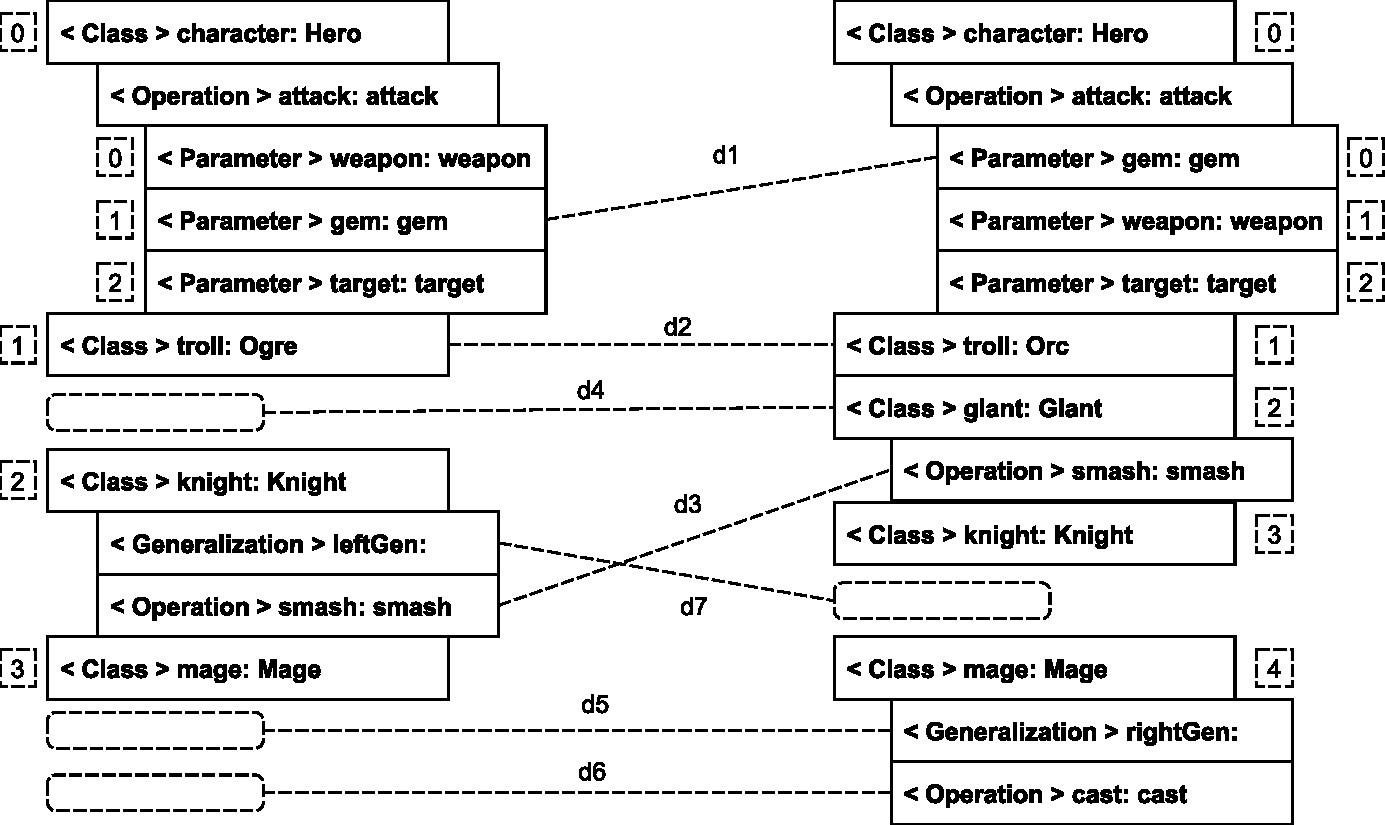
\includegraphics[width=\linewidth]{XmiComparison}
  \caption{A comparison of the left and right models in Listings \ref{lst:xmimodel_left} and \ref{lst:xmimodel_right}.}
  \label{fig:xmi_comparison}
\end{figure}

\vspace{-20pt}
\begin{lstlisting}[firstnumber=1,style=eol,caption={Diffs presented as change events.},label=lst:readable_diffs]
move gem in attack.parameters from 0 to 1
set troll.name from "Orc" to "Ogre"
remove smash from giant.operations at 0 composite c1
add smash to knight.operations at 0 composite c1
unset giant.name from "Giant" to null composite c2
remove giant from resource at 2 composite c2
delete giant composite c2
unset mage.generalization from rightGen to null composite c3
unset rightGen.general from character to null composite c3
delete rightGen composite c3
unset cast.name from "cast" to null composite c4
remove cast from mage.operations composite c4
delete cast composite c4
create leftGen type Generalization composite c5
set knight.generalization from null to leftGen composite c5
set leftGen.general from null to character composite c5
\end{lstlisting}

\section{Change-based Model Differencing}
\label{sec:change_based_approach_for_comparing_models}
Compared to the state-based model conflict detection of EMF Compare, the change-based model conflict detection proposed in this work consists of three phases: event loading, element tree construction, and conflict computation.
Conflict detection is not performed over all the elements of the model, as it is in state-based model differencing. Instead, this approach needs to compare only the last sets of change events of the two models, starting where the lines of the two models are different. A simplified class diagram of this approach \cite{epsilonlabs2019emfcbp} is depicted in Figure \ref{fig:approach_class_diagram}. The three phases are described in detail in the following sections.

\subsection{Event Loading}
\label{sec:event_loading}
In the event loading phase, the implementation loads change events recorded in two change-based model persistence files into memory.
The most important aspect of this phase is the partial loading, as only lines starting where the two files are different are loaded.
Thus, not the whole model needs to be traversed and loaded.
In this case, lines 1–29 in Listing \ref{lst:cbp_origin} are skipped. Only the lines starting with line 30 in Listings \ref{lst:cbp_left} and \ref{lst:cbp_right} are loaded. This yields two partial—left and right—change-event models.

\subsection{Element Tree}
\label{sec:tree_construction}
An element tree is a representation of the changes of model elements in the source and reference models. It contains detailed information about elements and their properties. It contains information similar to that captured in change lists in state-based model persistence, but it also provides more information about the changes. For example, the element tree can keep track of a feature’s old value and an element/value’s indexes inside multi-valued properties. The element tree contains only the partial states of affected elements of the original, left, and right models as depicted in Figures \ref{fig:left_element_tree_diagram} and \ref{fig:right_element_tree_diagram}.

To better understand the construction of an element tree from change events, we use the following running example using both change events in Listings \ref{lst:cbp_left} and \ref{lst:cbp_right}. We start from the left change events.

\subsubsection{Left Side}\label{sec:left_side}
In the first change event in Listing \ref{lst:cbp_left} at line \ref{line:cbp_left_30}, the change event is a \textsf{session} event. It indicates that all the following change events until the final line or next \textsf{session} event are persisted in one batch when they are saved. At line \ref{line:cbp_left_31}, we can see that Bob created a \textsf{Generalization} with ID \textsf{leftGen}. Thus, in \textsf{elementTree}, an element with ID \textsf{leftGen} also is created. To indicate that an element is newly created in the session, we put a ‘+’ sign at the left lower box of element \textsf{leftGen} in Figure \ref{fig:left_element_tree_diagram}.

\begin{landscape}
  \begin{figure}
    \includegraphics[width=\linewidth]{TreeClassDiagram}
    \caption{A class diagram showing the core components of the change-based approach to speed up model differencing and conflict detection.}
    \label{fig:approach_class_diagram}
  \end{figure}
\end{landscape}

\begin{figure}[ht]
  \centering
  \includegraphics[width=\linewidth]{element_tree_game_left}
  \caption{An element tree constructed from information in CBPs in Listing \ref{lst:cbp_left} (left change events only).}
  \label{fig:left_element_tree_diagram}
\end{figure}

At line \ref{line:cbp_left_32}, the feature \textsf{general} of \textsf{leftGen} is set to \textsf{character}. From the change event, we can recognise that \textsf{character} existed in the previous version since it has not been created in the current editing session. Thus, we create an element with ID \textsf{character} and the feature \textsf{general} of \textsf{leftGen} and put them in \textsf{elementTree}. We then set the value of \textsf{general} to \textsf{character} on the left side. We follow the same routine with \textsf{troll} and \textsf{generalization} at line \ref{line:cbp_left_33}, adding element \textsf{troll} and feature \textsf{generalization} to \textsf{elementTree} and setting the value of feature \textsf{generalization} to \textsf{leftGen} on the left side of the \textsf{elementTree}.

The change event at line \ref{line:cbp_left_34} changes \textsf{character}’s \textsf{name} from “Character” to “Hero”. From the change event, we can see that \textsf{character} existed before. Thus, we create element \textsf{character} and feature \textsf{name} into \textsf{elementTree}. We also set the value of \textsf{name} to “Hero” on the left side. Since this set change event is the first event for \textsf{character}’s \textsf{name}, we can infer that the original value of \textsf{name} is “Character”. Thus, we set \textsf{name}’s value to “Character” on the original side. The value of \textsf{name} on the right side also is set to “Character”, but it will be modified later when we process the right change events (Alice’s change events) if there is any change event that affects it. The same routine is applied when we process the change event at line \ref{line:cbp_left_43} later.

Lines \ref{line:cbp_left_35} and \ref{line:cbp_left_36} are the change events of composite move event \textsf{l1}. Element \textsf{leftGen} is removed (unset) from \textsf{troll}’s \textsf{generalization} and is assigned (set) to \textsf{knight}’s \textsf{generalization}. From these change events, we can see that element \textsf{knight} also existed in the original version. Thus, we add it into \textsf{elementTree} together with its \textsf{generalization} feature. Element \textsf{troll} and its \textsf{generalization} feature are not added into \textsf{elementTree} any more since they were added when processing line \ref{line:cbp_left_33}. In \textsf{elementTree}, we set \textsf{troll}’s \textsf{generalization} to null since element \textsf{leftGen} is moved to \textsf{knight}’s \textsf{generalization}.

At line \ref{line:cbp_left_37}, \textsf{target} is moved from index 1 to 2 in \textsf{attack}’s \textsf{parameters}. From the change event, we can see that element \textsf{target} has been contained in \textsf{attack}’s \textsf{parameters} at index 1 since the original version. Thus, we put element \textsf{target} and element \textsf{attack} and its \textsf{parameters} feature into \textsf{elementTree}. We also create a map on the left side with a key ‘2’ and a value that points to element \textsf{target} for feature \textsf{parameters}, indicating \textsf{target} is at index 2 in the left version. Since it is the first change event that moves \textsf{target}, we can decide that \textsf{target} is at index 1 in the original version. Thus, we create another map on the original side a map on the left side with a key ‘1’ and a value that also points to \textsf{target}. We also perform this routine to the right side of feature \textsf{parameters}, creating a map with a key ‘1’ and a value that also points to \textsf{target}. It will be modified later when we process the right change events (Alice’s change events) if there is any change event that affects the index of \textsf{target}.

Lines \ref{line:cbp_left_38} to \ref{line:cbp_left_42} are the change events of composite delete event \textsf{l2}; a deletion of element \textsf{giant}.
A deletion of an element unsets all the features of that element and its sub-elements, removes the sub-elements from their containers, and deletes the element and sub-elements from the model.
As can be seen, the value of \textsf{cast}’s \textsf{name} is unset from “cast” to null at line \ref{line:cbp_left_38}. From the change event, we know that cast has existed since the original version. Thus, we add element \textsf{cast} and its feature \textsf{name} to \textsf{elementTree} and set its value null on the left side and “cast” on the origin and right sides.

At line \ref{line:cbp_left_39}, \textsf{cast} is removed from \textsf{giant}’s \textsf{operations} at index 0. From it, we can see that \textsf{giant} and its feature \textsf{operations} exist, and \textsf{cast} is contained in \textsf{giant}’s \textsf{operations} at index 0 in the original version. Thus, we create element \textsf{giant} and its feature \textsf{operations} in \textsf{elementTree}. Three maps also are created in \textsf{operations} for the three sides. Each map contains a key ‘0’, indicating index, and a value that points to element \textsf{cast}—except on the left side the value is null since \textsf{cast} is removed from \textsf{giant}’s \textsf{operations}. The deletion of \textsf{cast} at line \ref{line:cbp_left_40} marks \textsf{cast} in \textsf{elementTree} with a ‘-’ sign on the left side to indicate that the element is deleted from the model in the left version.

Change event at line \ref{line:cbp_left_41} is similar to change event at line \ref{line:cbp_left_38}, except that it is applied to \textsf{giant}’s \textsf{name}. Since \textsf{giant} has existed in \textsf{elementTree}, only the feature \textsf{name} is added. Its value is set to null on the left side and “Giant” on the origin and right sides. The deletion of \textsf{giant} at line \ref{line:cbp_left_42} marks \textsf{giant} in \textsf{elementTree} with a ‘-’ sign to indicate that the element is deleted from the model in the left version.

Figure \ref{fig:left_element_tree_diagram} illustrates the state of the \textsf{elementTree} after all left change events have been processed. As can be seen, the \textsf{elementTree} exhibits the partial states of the original, left, and right models at once.

\subsubsection{Right Side}\label{sec:right_side}
In Listing \ref{lst:cbp_right}, similar to processing the left change events, the processing of the right change events (Alice’s version) starts with processing the session event at line \ref{line:cbp_right_30}. At line \ref{line:cbp_right_31}, \textsf{target} is moved from index 1 to 0 in \textsf{attack}’s \textsf{parameters}. Since the index of \textsf{target} is already determined when processing the change event, we determine the index of \textsf{target} only on the right side. We unset the value of key ‘1’ on the right side to null and create a new key ‘0’ that maps its value to \textsf{target}.

\begin{figure}[ht]
  \centering
  \includegraphics[width=\linewidth]{element_tree_game_right}
  \caption{An element tree constructed from information in CBPs in Listings \ref{lst:cbp_left} and \ref{lst:cbp_right} (all left and right change events).}
  \label{fig:right_element_tree_diagram}
\end{figure}

Composite move event \textsf{r1} at lines \ref{line:cbp_right_32} and \ref{line:cbp_right_33} moves \textsf{smash} from \textsf{knight}’s \textsf{operations} to \textsf{giant}’s \textsf{operations}. From this move event, we can see that \textsf{smash} is no longer in \textsf{knight}’s \textsf{operations}; it is contained in \textsf{giant}’s \textsf{operations} on the right side. Element \textsf{smash} has never existed in \textsf{elementTree}. So, we create and add \textsf{smash} to \textsf{knight}’s \textsf{operations} at index 0 on the origin side and to \textsf{giant}’s \textsf{operations} at index 0 on the right side. Since \textsf{smash} is not modified on the left side and no other change events applied to \textsf{knight}’s \textsf{operations}, we can determine that \textsf{smash} is at index 0 in \textsf{giant}’s \textsf{operations} on the left side.

Lines \ref{line:cbp_right_34} to \ref{line:cbp_right_35} are change events that constitute composite move event \textsf{r2}. This event moves \textsf{cast} from \textsf{giant}’s \textsf{operations} to \textsf{mage}’s \textsf{operations}. From this move event, we can see that \textsf{cast} is no longer in \textsf{giant}’s \textsf{operations} but now exists in \textsf{mage}’s \textsf{operations} on the right side. Element \textsf{mage} and its feature \textsf{operations} have never existed in \textsf{elementTree}. So, we create and add them to \textsf{elementTree} and add \textsf{cast} to \textsf{mage}’s \textsf{operations} on the right side.

At line \ref{line:cbp_right_36}, we can see that Alice created a \textsf{Generalization} with ID \textsf{rightGen}. Thus, in \textsf{elementTree}, an element with ID \textsf{rightGen} is created. Since it has just been created in the active session, the element is marked with a ‘+’ sign in \textsf{elementTree} on the right side. At line \ref{line:cbp_right_37}, we can also see that feature \textsf{general} should be added to \textsf{rightGen} in \textsf{elementTree} and the value is set to \textsf{character} on the right side. We also set \textsf{mage}’s \textsf{operations} to \textsf{rightGen} on the right side of \textsf{elementTree} according to the change event at line \ref{line:cbp_right_38}.

Change event at line \ref{line:cbp_right_39} changes \textsf{character}’s \textsf{name} from “Character” to “Hero”. Since \textsf{character} and its feature \textsf{name} already exist in \textsf{elementTree}, we set \textsf{name}’s value to “Hero” only on the right side. The original value was already assigned when processing left change events. We apply the same routine when processing the change event at line \ref{line:cbp_right_42} later.



Composite move event \textsf{r3} at lines \ref{line:cbp_right_40} and \ref{line:cbp_right_41} moves \textsf{rightGen} from \textsf{troll}’s \textsf{generalization} to \textsf{mage}’s \textsf{generalization}. From this move event, on the right side, we can see that \textsf{rightGen} is no longer in \textsf{troll}’s \textsf{generalization} but exists in \textsf{mage}’s \textsf{generalization}. Since it is the first time \textsf{mage}’s \textsf{generalization} is modified, we create and add the feature to \textsf{mage} in \textsf{elementTree}. On the right side of \textsf{elementTree}, we unset \textsf{troll}’s \textsf{generalization} to null and assign \textsf{rightGen} to \textsf{mage}’s \textsf{generalization}.

Figure \ref{fig:right_element_tree_diagram} exhibits the state of the \textsf{elementTree} after both sides’ change events have been processed.

\subsubsection{Construction Procedure}\label{sec:construction_procedure}

The construction of \textsf{elementTree} follows the steps shown in Figure \ref{fig:tree_construction}. First, the partial state $S_{L}$ of the left model in the \textsf{elementTree} is constructed based on the information retrieved from the left change events (step 1). We denote this information as $I_{LL}$. We can also construct the partial state $S_{O}$ of the original model using the information about the original state contained in the left change events $I_{OL}$ (step 2). The information $I_{OL}$ allows us to construct the initial partial state $S_{R}$ of the right model (step 3). Similarly, using the information from the right change events $I_{RR}$, we update the partial right state $S_{R}$, which was initialised before using the information $I_{OL}$ (step 4), implying that $I_{OL} \cup I_{RR} \rightarrow S_{R}$. Also, information about the original model from the right change events $I_{OR}$ is used to update the original state (step 5). Thus, we have constructed a partial state of the original model using information from both left and right sides, $I_{OL} \cup I_{OR} \rightarrow S_{O}$. Finally, we also use the information $I_{OR}$ to update the partial state of the left model (step 6), implying that $I_{LL} \cup I_{OR} \rightarrow S_{L}$.

\begin{figure}[ht]
  \centering
  \includegraphics[width=\linewidth]{TreeConstruction}
  \caption{Steps in Element Tree construction.}
  \label{fig:tree_construction}
\end{figure}

Algorithm \ref{alg:element_tree} describes the steps presented in Figure \ref{fig:tree_construction} in a generic fashion. It iterates through all of a model’s change events and uses the information contained in them to construct the relevant partial state. The choice to begin with left or right change events depends on the \textsf{Side} enumeration value—\textsf{left} or \textsf{right}—passed through the parameter \textsf{side} (the second input parameter). In our implementation, we process the left side first by default. The algorithm also receives an input of the change events \textsf{events} that are to be iterated and the element tree \textsf{elementTree} that has been instantiated. Then it returns the \textsf{elementTree} as output after updating it.

For each \textsf{event} in the \textsf{events}, we collect information needed to build up \textsf{elementTree} (lines 3–9), such as \textsf{targetElement}, \textsf{feature}, \textsf{value}, \textsf{previousValue}, \textsf{index}, and \textsf{previousIndex}. The \textsf{targetElement} is the element modified by a change event (e.g., \textsf{character} and \textsf{giant} in Listing \ref{lst:cbp_left}). This \textsf{targetElement}—an instance of class Element in Figure \ref{fig:approach_class_diagram}—is retrieved from the \textsf{elementTree} if it already exists. Otherwise, a new element is created and added to the \textsf{elementTree} (line 3). In this step we also set the flags \textsf{*IsCreated} and \textsf{*IsDeleted} of the element in Figure \ref{fig:approach_class_diagram}. For example, if the type of the event is \textsf{create} then \textsf{*IsCreated} is set to \textsf{true}. The \textsf{feature}—an instance of class Feature in Figure \ref{fig:approach_class_diagram}—represents the target element’s feature (e.g., \textsf{name} and \textsf{operations} in Listing \ref{lst:cbp_right}) modified by a change event. It is retrieved from the \textsf{targetElement}’s feature list, and a new one is created and added to the \textsf{targetElement}’s feature list if the feature does exist (line 5).

The \textsf{value} is the value assigned to the feature in a change event (line 5, Algorithm \ref{alg:element_tree}). The \textsf{value} can be a type of \textsf{Element} (e.g., element \textsf{leftGen} line \ref{line:cbp_left_36} in Listing \ref{lst:cbp_left}) or primitive (e.g., the string “Hero” at line \ref{line:cbp_left_34} in Listing \ref{lst:cbp_left}). The \textsf{previousValue} represents the previous value of the modified feature (line 6, Algorithm \ref{alg:element_tree}). The \textsf{previousValue} is not defined if no previous value has been assigned. For \textsf{value} and \textsf{previousValue} with type \textsf{Element}, the elements they represent are retrieved from the \textsf{elementTree}, and if they do not exist, new instances are created. If the type is primitive, the value is treated as it is. Not every change event has a \textsf{value}, particularly events with type \textsf{create}
or \textsf{delete}, which modify only a target element not an element feature.

\IncMargin{1.5em}
\begin{algorithm}[H]
  \begin{footnotesize}
    \SetKwInOut{Input}{input}
    \SetKwInOut{Output}{output}
    \Input{a list of ChangeEvent $events$}
    \Input{an enumeration of Side $side$}
    \Input{an instance of ElementTree $elementTree$}
    \Output{an instance of ElementTree $elementTree$}
    \SetKwBlock{Beginn}{beginn}{ende}
    \Begin{
      \ForEach{$event$ in $events$}{
        $targetElement$ $\leftarrow$ getOrCreateNewTargetElement($event$, $elementTree$)\;
        $feature$ $\leftarrow$ getOrCreateNewFeature($event$, $targetElement$)\;
        $value$ $\leftarrow$ getValue($event$)\;
        $previousValue$ $\leftarrow$ getPreviousValue($event$)\;
        $index$ $\leftarrow$ getIndex($event$)\;
        $previousIndex$ $\leftarrow$ getPreviousIndex($event$)\;
        $featureEventList$ $\leftarrow$ getFeatureEventList($feature$, $side$)\;
        
        \BlankLine
        \tcp{put all values to their proper indexes}
        updateTree($targetElement$, $feature$, $value$, $index$, $side$)\;
        $oldIndexes$ $\leftarrow$ calculateOldIndex($featureEventList$, $previousIndex$, $side$)\;
        \If{\Not isCreated($value$, $side$) \AndA \Not isOldValueSet($feature$, $previousValue$, $previousIndex$, $side$)} {
          setOldValue($feature$, $previousValue$, $oldIndex$, $side$)\;
          $oppositeFeatureEventList$ $\leftarrow$ getOppositeFeatureEventList($feature$, $side$)\;
          $oppositeIndex$ $\leftarrow$ calculateOppositeIndex($oppositeFeatureEventList$, $oldIndex$, $side$)\;
          \If{\Not isDeleted($value$, $side$) \AndA \Not isOppositeSideValueSet($feature$, $value$, $oppositeIndex$, $side$)} {
            setOppositeSideValue($feature$, $value$, $oppositeIndex$, $side$)\;
          }
        }
        
        addEventToFeatureEventList($event$, $featureEventList$)\;
        
      }
      \Return{$elementTree$}\;
    }
  \end{footnotesize}
  \caption{Algorithm to construct an element tree from events.}
  \label{alg:element_tree}
\end{algorithm}
\DecMargin{1.5em}



The \textsf{index} is the index assigned by a change event to a value in a feature, while \textsf{previousIndex} is the previous index of the value (lines 7–8, Algorithm \ref{alg:element_tree}). In one change event, we can get both \textsf{index} and \textsf{previousIndex} or only one of them, depending on the type of the change event. For example, we can determine that the \textsf{index} of \textsf{cast} is 0 (line \ref{line:cbp_right_35} in Listing \ref{lst:cbp_right}) because the change event type is \textsf{add}. In a \textsf{remove} change event, we can get only the \textsf{previousIndex} of \textsf{cast}, which is 1 (line \ref{line:cbp_right_35} in Listing \ref{lst:cbp_right}), because the element does not exist anymore in the left model. We can obtain both of them only in a \textsf{move} change event as an element is moved from a previous index to a new one (line \ref{line:cbp_right_31} in Listing \ref{lst:cbp_right}). For a single-valued feature, the \textsf{index} and \textsf{previousIndex} are always 0, because the feature can contain only a single value.

At line 9, we retrieve the \textsf{featureEventList} from the \textsf{feature} to be added later with the current \textsf{event} (line 19). The \textsf{featureEventList} is a list—a history—of change events that have been processed that are specific to the \textsf{feature} on the selected \textsf{side}. Using the obtained \textsf{targetElement}, \textsf{feature}, \textsf{value}, and \textsf{index}, the process then updates the state of the \textsf{elementTree} on the selected \textsf{side} (line 10). After that, it calculates the original index of a value, using the \textsf{featureEventList} and \textsf{previousIndex} (line 11). If the value at \textsf{oldIndex} in the \textsf{feature} has not been set, then the algorithm sets the \textsf{feature} with the \textsf{previousValue} at the \textsf{oldIndex} in the partial state of the original model (lines 12–13). At lines 14–18, the algorithm does the same thing to the opposite side—if the current \textsf{side} is \textsf{left} then it is \textsf{right}.

\subsection{Diff Computation}
\label{sec:diff_computation}
Using the \textsf{elementTree} presented in Figure \ref{fig:right_element_tree_diagram}, we can determine the difference between the left and right models without having to compare all their elements and features. After the \textsf{elementTree} has been constructed, we iterate through elements and features of the \textsf{elementTree} and use the flags, containers, containing features, and indexes on both sides of each element and value to identify differences between the left and right models. We follow the steps in Algorithm \ref{alg:diff_calculation}. The algorithm visits each element and every index of each feature (lines 3–5). At every index, it retrieves the \textsf{leftValue} and \textsf{rightValue} (lines 5–7), passing these, together with the \textsf{element}, \textsf{feature}, and \textsf{index} to a function \textsf{identifyDiffUsingRules} (line 8). The function uses a set of pre-defined rules to identify the differences \textsf{diffs} based on the states of flags of an element, flags and attributes of the element’s feature, values of the feature, and indexes of the values. The obtained \textsf{diffs} are then added to the overall list of differences \textsf{diffList} which is output (line 8–9, 13).

\IncMargin{1.5em}
\begin{algorithm}[H]
  \begin{footnotesize}
    \SetKwInOut{Input}{input}
    \SetKwInOut{Output}{output}
    \Input{an instance of ElementTree $elementTree$}
    \Begin{
      $diffList$ $\leftarrow$ DiffList()\;
      \ForEach{$element$ \In $elementTree$}{
        \ForEach{$feature$ \In getFeatures($element$)}{
          \ForEach{$index$ \In getIndexes($feature$)}{
            $leftValue$ $\leftarrow$ getLeftValue($feature$, $index$)\;
            $rightValue$ $\leftarrow$ getRightValue($feature$, $index$)\;
            \BlankLine
            \tcp{rules starts from here}
            $diffs$ $\leftarrow$ identifyDiffUsingRules($element$, $feature$, $leftValue$, $rightValue$, $index$)\;
            addToDiffList($diffs$,$diffList$)\;
          }
        }
      }
      \Return{$diffList$}\;
    }
  \end{footnotesize}
  \caption{Algorithm to determine differences.}
  \label{alg:diff_calculation}
\end{algorithm}
\DecMargin{1.5em}

We illustrate the principles and the use of rules by discussing the rules used to identify differences in the running example. These can be found in Algorithm \ref{alg:diff_rules}. The algorithm is the breakdown of the function \textsf{identifyDiffUsingRules} in Algorithm \ref{alg:diff_calculation}. As previously stated, it is important to remember that we use the left model as a reference, which means the differences are presented as changes that transform the right model to become equal to the left model.

\IncMargin{1.5em}
\begin{algorithm}[]
  \begin{footnotesize}
    \SetKwInOut{Input}{input}
    \SetKwInOut{Output}{output}
    \Input{an Element $element$, a Feature $feature$, a variable $leftValue$, a variable $rightValue$, an Integer $index$}
    \Output{a List of Diff $diffs$}
    $diffs$ $\leftarrow$ createDiffList()\;
    \tcp{...}
    \tcp{Rule 1: a rule to determine a change of a single-valued attribute}
    \If{getType($feature$) \Is Attribute \AndA isSingleValued($feature$) \AndA leftValue <> rightValue \AndA \Not leftIsCreated($element$) \AndA \Not leftIsDeleted($element$) \AndA \Not rightIsCreated($element$) \AndA \Not rightIsDeleted($element$)}{
      $diff$ $\leftarrow$ createNewDiff($element$, $element$, $feature$, $feature$, $index$, $index$, $leftValue$, $rightValue$, DifferenceType.CHANGE)\;
      addDiffToDiffList($diff$, $diffs$)\;
    }
    \tcp{Rule 2: A rule to determine movement of an element for right value (the left value has its own rule)}
    \If{getType($feature$) \Is Containment \AndA \Not isNull($rightValue$) \AndA \Not leftIsCreated($rightValue$) \AndA \Not leftIsDeleted($rightValue$) \AndA \Not rightIsCreated($rightValue$) \AndA \Not rightIsDeleted($rightValue$) \AndA (getLeftContainer($rightValue$) <> getRightContainer($rightValue$) \Or getLeftFeature($rightValue$) <> getRightFeature($rightValue$) \Or getLeftIndex($rightValue$) <> getRightIndex($rightValue$))}{
      $diff$ $\leftarrow$ createNewDiff(getLeftContainer($rightValue$), getRightContainer($rightValue$), getLeftFeature($rightValue$), getRightFeature($rightValue$), getLeftIndex($rightValue$), getRightIndex($rightValue$), $rightValue$, $rightValue$, DifferenceType.MOVE)\;
      addDiffToDiffList($diff$, $diffs$)\;
    }
    \tcp{Rule 3: The first of two rules to determine the deletion of an element}
    \If{getType($feature$) \Is Containment \AndA \Not leftIsCreated($rightValue$) \AndA leftIsDeleted($rightValue$) \AndA \Not rightIsCreated($rightValue$) \AndA \Not rightIsDeleted($rightValue$) }{
      createNewDiff(getLeftContainer($rightValue$), getRightContainer($rightValue$), getLeftFeature($rightValue$), getRightFeature($rightValue$), null, getRightIndex($rightValue$), null, $rightValue$, DifferenceType.DELETE)\;
      addDiffToDiffList($diff$, $diffs$)\;
    }
    \tcp{...}
    \tcp{continue to part 2}
  \end{footnotesize}
  \caption{Some rules to determine differences (part 1).}
  \label{alg:diff_rules}
\end{algorithm}
\DecMargin{1.5em}

The first rule (Rule 1) in Algorithm \ref{alg:diff_rules} is to identify changes in single-valued attributes. A feature must be of type \textsf{attribute}, both side values must be different, and the element should have not been created or deleted in both models. The second rule (Rule 2) identifies whether an element is in a different location in the two models. The element must not have been deleted, and it must exist from the previous version—the original model. Also, the containers, containing features, or indexes of the element must be different on the two sides. The third rule (Rule 3) identifies the deletion of an element. If an element in the left model is not created but exists in the model, it means that the element has existed since the previous version—the original model. This also means that the element also exists in the right model, unless it has been deleted. Thus, to make the right model equal to the left model, the element must be deleted in the right model as well.

\IncMargin{1.5em}
\begin{algorithm}[H]
  \begin{footnotesize}
    \tcp{continuation of part 1}
    \tcp{...}
    \tcp{Rule 4: The second of two rules to determine deletion of an element}
    \If{getType($feature$) \Is Containment \AndA \Not leftIsCreated($rightValue$) \AndA \Not leftIsDeleted($rightValue$) \AndA rightIsCreated($rightValue$) \AndA rightIsDeleted($rightValue$) }{
      createNewDiff(getLeftContainer($rightValue$), getRightContainer($rightValue$), getLeftFeature($rightValue$), getRightFeature($rightValue$), null, getRightIndex(rightValue), null, $rightValue$, DifferenceType.DELETE)\;
      addDiffToDiffList($diff$, $diffs$)\;
    }
    \tcp{Rule 5: one of rules to determine addition of an element}
    \If{getType($feature$) \Is Containment \AndA leftIsCreated($leftValue$) \AndA \Not leftIsDeleted($leftValue$) \AndA \Not rightIsCreated($leftValue$) \AndA \Not rightIsDeleted($leftValue$)}{
      $diff$ $\leftarrow$ createNewDiff(getLeftContainer($leftValue$), getRightContainer($leftValue$), getLeftFeature($leftValue$), getRightFeature($leftValue$), getLeftIndex($leftValue$), null, $rightValue$, null, DifferenceType.ADD)\;
      addDiffToDiffList($diff$, $diffs$)\;
    }
    \tcp{...}
    \Return{$diffs$}
  \end{footnotesize}
  \caption{Some rules to determine differences (part 2).}
  \label{alg:diff_rules_2}
\end{algorithm}
\DecMargin{1.5em}

The fourth rule (Rule 4) in Algorithm \ref{alg:diff_rules_2} also identifies the deletion of an element. The element never existed in the left model, but it has been created in the right model. Thus, to make the right model equal to the left model, the element must be deleted from the right model. The fifth rule (Rule 5) identifies the need to add an element. If an element is created in the left model and has not been deleted, it means that the element should be added to the right model to make the two models equal.

In Figure \ref{fig:right_element_tree_diagram}, when the iteration of \textsf{elementTree}, from element \textsf{character} down to feature \textsf{name} of element \textsf{cast} reaches index 0 in feature \textsf{parameters} of element \textsf{attack}, we can see that \textsf{rightValue} has the value element \textsf{target} and the value of \textsf{leftValue
} is unknown. The \textsf{rightValue} is not null and value \textsf{target} exists on both sides—all its \textsf{*Created} and \textsf{*Deleted} flags are false, and it also different indexes (2 in the left state and 0 in the right state). This meets the condition of the second rule. Thus, we can conclude that, to make the index of element \textsf{target} in the right model equal its index in the left model, element \textsf{target} should be moved from index 0 to 2. Thus, the type of this difference is \textsf{MOVE}. We denote this difference as $dc_{1}$. The same rule is applied to element \textsf{smash} when the iteration reach index 0 in \textsf{knight}’s \textsf{generalization}. Applying the rule to the element produces difference $dc_{3}$.

When the iteration is at feature \textsf{name} of element \textsf{troll}, we determine that the type of the feature is a single-valued attribute and the sides of the feature are different in value. This means that the condition of the first rule is met. Thus, we can conclude that, to make the left value of the feature equal to the right value, we must override the value “Orc” with “Ogre”. The type of this difference is \textsf{CHANGE}. We denote this difference as $dc_{2}$.

At \textsf{giant}, the element used to exist but it has been deleted from the left model (flags \textsf{leftIsCreated} = false, \textsf{leftIsDeleted} = true); it still exists in the right state (flags \textsf{rightIsCreated} = false, \textsf{rightIsDeleted} = false). This condition satisfies the third rule. Therefore, element \textsf{giant} should be deleted from the right model. The type of this difference is \textsf{DELETE}. We denote this difference as $dc_{4}$. The same rule is applied to element \textsf{cast} when the iteration reaches the element. Applying the rule to the element produces difference $dc_{6}$.

We can get only one value when the iteration is at index 0 in the element \textsf{knight}’s feature \textsf{generalization}; the \textsf{leftValue} is element \textsf{leftGen}, but the \textsf{rightValue} is unidentified. Thus, we process only the \textsf{leftValue}. Element \textsf{leftGen} is created only in the left model (flags \textsf{leftIsCreated} = true, \textsf{leftIsDeleted} = false, \textsf{rightIsCreated} = false, \textsf{rightIsDeleted} = false). This meets the condition of the fifth rule. Thus, to make element \textsf{leftGen} exist in the right state, we must add it into element \textsf{knight}’s feature \textsf{generalization} at index 0. Therefore, the type of this difference is \textsf{ADD}. We denote this difference as $dc_{7}$.

When the iteration is at index 0 in the element \textsf{mage}’s feature \textsf{generalization}, we can get only one value; the \textsf{leftValue} is unidentified and the \textsf{rightValue} is element \textsf{rightGen}. Therefore, we process only the \textsf{rightValue}. Element \textsf{rightGen} is created only in the right model (flags \textsf{leftIsCreated} = false, \textsf{leftIsDeleted} = false, \textsf{rightIsCreated} = true, \textsf{rightIsDeleted} = false). This meets the condition of the fourth rule. Thus, to make element \textsf{rightGen} cease to exist in the left state, we must delete it from index 0 in element \textsf{mage}’s feature \textsf{generalization}. Therefore, the type of this difference is \textsf{DELETE}. We denote this difference as $dc_{5}$.



Similar to the state-based approach in Section \ref{sec:state-based_model_differencing}, we express identified differences as $dc_{n}$ = [$LeftContainer_n$, $RightContainer_n$, $LeftFeature_n$, $RightFeature_n$, $LeftIndex_n$, $RightIndex_n$, $LeftValue_n$, $RightValue_n$, $Kind_n$]. Thus:

$dc_{1}$ = [\textsf{attack}, \textsf{attack}, \textsf{parameters}, \textsf{parameters}, 2, 0, \textsf{target}, \textsf{target}, \textsf{MOVE}]\\
$dc_{2}$ = [\textsf{troll}, \textsf{troll}, \textsf{name}, \textsf{name}, 0, 0, “Ogre”, “Orc”, \textsf{CHANGE}]\\
$dc_{3}$ = [\textsf{knight}, \textsf{giant}, \textsf{operations}, \textsf{operations}, 0, 0, \textsf{smash}, \textsf{smash}, \textsf{MOVE}]\\
$dc_{4}$ = [\textsf{resource}, \textsf{resource}, \textsf{null}, \textsf{null}, \textsf{null}, 2, \textsf{null}, \textsf{giant}, \textsf{DELETE}]\\
$dc_{5}$ = [\textsf{mage}, \textsf{mage}, \textsf{generalization}, \textsf{generalization}, \textsf{null}, 0, \textsf{null}, \textsf{rightGen}, \textsf{DELETE}] \\
$dc_{6}$ = [\textsf{mage}, \textsf{mage}, \textsf{operations}, \textsf{operations}, \textsf{null}, 0, \textsf{null}, \textsf{cast}, \textsf{DELETE}]\\
$dc_{7}$ = [\textsf{knight}, \textsf{knight}, \textsf{generalization}, \textsf{generalization}, 0, \textsf{null}, \textsf{leftGen}, \textsf{null}, \textsf{ADD}]

This change-based approach might produce differences that are distinct from differences identified using state-based approaches. This can be seen by comparing $ds_{1}$ and $dc_{1}$ ($ds_{1}$ $\neq$ $dc_{1}$, [\textsf{attack}, \textsf{attack}, \textsf{parameters}, \textsf{parameters}, 0, 1, \textsf{gem}, \textsf{gem}, \textsf{MOVE}] $\neq$ [\textsf{attack}, \textsf{attack}, \textsf{parameters}, \textsf{parameters}, 2, 0, \textsf{target}, \textsf{target}, \textsf{MOVE}]). The state-based approach identifies element \textsf{gem} as the element that should be moved to index 0 to resolve the differences in \textsf{attack}’s \textsf{parameters} ($ds_{4}$), while in the change-based approach, the difference is attributed to element \textsf{target} ($dc_{4}$). However, in both approaches, if we resolve their differences by performing all-left-to-right merging—making the right model equal to the left model, the two approaches produce models that are equivalent. In this way, we can check the correctness of the identified differences produced by the change-based approach.

\vspace{-10pt}
\section{Evaluation}
\label{sec:evaluation_6}
This section presents the method used to evaluate the proposed change-based model differencing approach as well as the evaluation results.

\subsection{Method}
\label{sec:method}
To assess the performance benefits of the change-based approach in terms of model differencing, we have evaluated it against a mature and widely used state-based comparison tool (EMF Compare \cite{emfcompare2018developer, eclipse2017compare}). Since there are no large, manually developed models persisted in our change-based format yet, the dataset for our experiments was constructed from a large model reverse-engineered from the Eclipse Epsilon project \cite{eclipse2018epsilongit, eclipse2017epsilon}. This model conforms to the Java meta-model \cite{eclipse2018modiscojava}, and it consists of more than 1.6 million elements with a size of 224 MB when persisted in XMI.

We cloned the original model to produce two new (left and right) models and performed operations (\textsf{add}, \textsf{remove}, \textsf{move}, \textsf{set} with random elements, features, indexes, and values) on both models to create differences. We made 1.1 million artificial changes to each model, generating over 1.1 million events (one operation can generate more than one event, e.g., a \textsf{move} between features generates \textsf{remove} and \textsf{add} events). Events generated by the changes were persisted in our change-based format (to be used later in change-based model differencing). After every 50,000 changes, we set a measurement point. We persisted the last state of the models in state-based format (to be used later in state-based model differencing) and then performed change-based and state-based model differencing and measured their execution time and memory footprint. We created 22 measurement points to capture their trends in one experiment.

We conducted five experiments. In the first experiment, the ratio of occurrence between \textsf{add}, \textsf{remove}, \textsf{move}, and \textsf{set} changes was set to 1:1:20:40. This reflects an assumption that in a mature model, modification—\textsf{move} and \textsf{set} events—occurs more frequently than addition and deletion. So the change of total elements does not affect our measurement, the number of total elements should be kept constant. For example, it is difficult to determine if an increase of time in comparison is caused by an increase in the number of elements or by the number of change events. One way to do this is to exclude \textsf{add} and \textsf{remove} operations. However, excluding both operations made measurement less representative. Thus, we included both operations, but we made their probabilities equal so that the number of total elements remains largely unchanged. 
In the rest of the experiments, we performed only homogeneous operations—isolated from other types—per experiment (e.g., add-only, move-only operations). In the end, we obtained five results: mixed, add-only, remove-only, move-only, and set-only measurements. We did this to assess whether operations of different types have different impacts on model differencing.

For the change-based approach, the comparison time comprises loading change events, constructing an element tree, and identifying differences. The memory footprint is the space used to hold the change events, element tree, and differences in memory. For state-based EMF Compare, the comparison time comprises matching elements and identifying differences, and the memory footprint is the space required to hold the matches and differences in memory. All measurements were performed on the same machine with the following specification: AMD Opteron(tm) Processor 6386 SE @ 2.8 GHz cache size 2 GB (64 processors), 528 GB main memory, Ubuntu 16.04.6 LTS operating system, and Java(TM) SE Runtime Environment (build 1.8.0\_201-b09) with JVM \textsf{InitialHeapSize} 2 GB and \textsf{MaxHeapSize} 32 GB.

\subsection{Results and Discussion}
\label{sec:results_and_discussion}

\begin{wrapfigure}[9]{r}{0.5\textwidth}
  \vspace{-20pt}
  \includegraphics[width=\linewidth]{mixed-count-events}
  \caption{total elements, affected elements, and diffs}
  \label{fig:modification_course}
\end{wrapfigure}

This section reports on the results for comparison time and memory footprint for the mixed and homogeneous operation experiments.

\vspace{-5pt}
\subsubsection{Mixed Operations}
\label{sec:mixed-operation}
In the mixed operation measurement, we modify two identical models differently by applying random operations. As the number of change events generated by the modification grows, the numbers of affected elements and differences also increase in a logarithmic manner. The patterns are shown in Figure \ref{fig:modification_course}. The growth is logarithmic since the probability that the random operations modify the same elements also increases. Thus, some change events might not add new affected elements and differences. In other words, more events are required to increase the number of affected elements or differences. In Figure \ref{fig:modification_course}, the total number of elements remains largely unchanged because the probabilities of addition and deletion were made equal, as noted in Section \ref{sec:evaluation_6}. The figure gives us an insight about the characteristics of the modification caused by the random operations in the mixed operation measurement; it helps to explain the implications of the changes on execution time and memory footprints of model differencing.

\begin{figure}[ht]
  \begin{subfigure}[t]{0.495\linewidth}
    \includegraphics[width=\linewidth]{mixed-time-events}
    \caption{execution time}
    \label{fig:time_diffs}
  \end{subfigure}
  \begin{subfigure}[t]{0.495\linewidth}
    \includegraphics[width=\linewidth]{mixed-memory-events}
    \caption{memory footprint}
    \label{fig:memory_diffs}
  \end{subfigure}
  \caption{Change-based vs. state-based model differencing as differences increase.}
  \label{fig:change_vs_state}
\end{figure}

\begin{figure}[ht]
  \centering
  \begin{subfigure}[t]{0.495\linewidth}
    \includegraphics[width=\linewidth]{mixed-time-events-detail}
    \caption{change-based comparison time}
    \label{fig:time_changediff_detail}
  \end{subfigure}
  \hfill
  \begin{subfigure}[t]{0.495\linewidth}
    \includegraphics[width=\linewidth]{state-time-events-detail}
    \caption{state-based comparison time}
    \label{fig:time_statediff_detail}
  \end{subfigure}
  \begin{subfigure}[t]{0.495\linewidth}
    \includegraphics[width=\linewidth]{mixed-memory-events-detail}
    \caption{change-based memory footprint}
    \label{fig:memory_changediff_detail}
  \end{subfigure}
  \hfill
  \begin{subfigure}[t]{0.495\linewidth}
    \includegraphics[width=\linewidth]{state-memory-events-detail}
    \caption{state-based memory footprint}
    \label{fig:memory_statediff_detail}
  \end{subfigure}
  \caption{Breakdown view of comparison time and memory footprint in Figure \ref{fig:change_vs_state}.}
  \label{fig:time_memory_detail}
\end{figure}

After applying some random changes on both models, the modification produces 100,000 change events at the first measurement point. Using this amount of events, our change-based comparison takes only 5 seconds to identify around 90,000 differences, in contrast to state-based comparison, which takes 66 seconds (see the first measurement points in Figures \ref{fig:modification_course} and \ref{fig:time_diffs}). If the modification continues, more change events are generated. This growing number of change events must be loaded into memory and thus slows down the change-based comparison. Nevertheless, change-based comparison is still faster than state-based comparison. Even when the number of change events reaches 2.37 million—more than 1 million differences  change-based comparison outperforms state-based comparison in execution time (Figure \ref{fig:time_diffs}). Figure \ref{fig:time_changediff_detail} presents the comparison time in detail. It shows that the event loading time is the dominant contributor to the slowdown compared to the element tree’s construction time and diffing time.

For the state-based comparison in Figure \ref{fig:time_statediff_detail}, the comparison time experiences only a slight increase as the number of identified differences also grows.
%\dk{Change to ‘grows’?}
This slight increase comes mainly from the diffing time, while the matching time tends to be constant because of the very small increase of total elements (Figures \ref{fig:modification_course}).

Nevertheless, a change-based comparison generally consumes more memory than a state-based comparison (see Figure \ref{fig:memory_diffs}). It consumes less memory than its state-based counterpart only when the number of events is fewer than 0.3 million. (At that moment there are fewer than 0.25 million identified differences.) Figure \ref{fig:memory_changediff_detail} separates the memory footprint of the change-based comparison into three factors: the loaded change events, element tree, and diffs. As modification continues, more events are generated. These events must be loaded into memory since they contain the information needed to construct an element tree. The amount of space to keep these change events in memory grows linearly with their number.

In contrast, the memory used for the element tree grows logarithmically. As the number of events increases, the probability that events modify already affected elements also increases. Thus, no additional memory allocation is required for the element tree. Moreover, the element tree occupies most of the memory footprint since it mirrors the partial states—elements, features, and values—of the models that are affected by the changes. In our technical implementation, a feature can have many instances—one instance for each element. (As a comparison, in the EMF implementation, there is only one instance for a feature. The feature is used as a key so that different elements can have the same feature that maps to different values simultaneously). This contributes to the large memory footprint used by the element tree. The identified change-based diffs, the third factor, are the smallest factor that contributes to the memory footprint of the change-based comparison.

\begin{figure}[ht]
  \centering
  \begin{subfigure}[t]{0.495\linewidth}
    \includegraphics[width=\linewidth]{add-time-events}
    \caption{add-only}
    \label{fig:add-time-events}
  \end{subfigure}
  \hfill
  \begin{subfigure}[t]{0.495\linewidth}
    \includegraphics[width=\linewidth]{delete-time-events}
    \caption{delete-only}
    \label{fig:delete-time-events}
  \end{subfigure}
  \begin{subfigure}[t]{0.495\linewidth}
    \includegraphics[width=\linewidth]{move-time-events}
    \caption{move-only}
    \label{fig:move-time-events}
  \end{subfigure}
  \hfill
  \begin{subfigure}[t]{0.495\linewidth}
    \includegraphics[width=\linewidth]{change-time-events}
    \caption{change-only}
    \label{fig:change-time-events}
  \end{subfigure}
  \caption{Comparison time for homogeneous operations.}
  \label{fig:operation_time_events}
\end{figure}



For the state-based comparison in Figure \ref{fig:memory_statediff_detail}, the memory footprint grows only slightly with the increase of differences. A large part of the memory footprint is used to represent the identified differences, while the memory used for matches tends to be constant, because the changes of the total elements are very few—fewer new elements means less memory must be allocated for new matches (Figures \ref{fig:modification_course}).


\subsubsection{Homogeneous Operations}
\label{sec:homogeneous-operation}

\begin{figure}[ht]
  \centering
  \begin{subfigure}[t]{0.495\linewidth}
    \includegraphics[width=\linewidth]{add-memory-events}
    \caption{add-only}
    \label{fig:add-memory-events}
  \end{subfigure}
  \hfill
  \begin{subfigure}[t]{0.495\linewidth}
    \includegraphics[width=\linewidth]{delete-memory-events}
    \caption{delete-only}
    \label{fig:delete-memory-events}
  \end{subfigure}
  \begin{subfigure}[t]{0.495\linewidth}
    \includegraphics[width=\linewidth]{move-memory-events}
    \caption{move-only}
    \label{fig:move-memory-events}
  \end{subfigure}
  \hfill
  \begin{subfigure}[t]{0.495\linewidth}
    \includegraphics[width=\linewidth]{change-memory-events}
    \caption{change-only}
    \label{fig:change-memory-events}
  \end{subfigure}
  \caption{Memory footprint for homogeneous operations.}
  \label{fig:operation_memory_events}
\end{figure}

Figures \ref{fig:operation_time_events} and \ref{fig:operation_memory_events} show the comparison times and memory footprints of models modified using homogeneous operations—\textsf{add}, \textsf{remove}, \textsf{move}, or \textsf{set} only. In all these figures, change-based comparison outperforms its state-based counterpart, particularly when the number of change events is small relative to the size of the model. As the number of modifications grows, change-based comparison becomes slower than state-based comparison. In our experiments, this happens when the number of events is greater than 4 million (Figure \ref{fig:add-time-events}). Change-based comparison also becomes slower when the size of models shrinks (because of a large number of delete events) as depicted in Figure \ref{fig:delete-memory-events}. This is because change-based comparison still needs to load these change events and construct its element tree. In contrast, deletion means less work for state-based comparison. In terms of memory footprint, change-based comparison performs better than state-based comparison only when the number of change events is fewer than 0.3 million, as depicted in Figure \ref{fig:operation_memory_events}.




\section{Conclusions}
\label{sec:conclusions_6}
This chapter proposed an approach to identify differences between two versions of a model persisted in change-based format. It works by loading into memory the changes made to both versions since the last shared version, constructing partial states of the versions based on the information in the latest changes, and using specific rules to identify differences between the versions’ elements and features.

The evaluation indicates that the change-based comparison approach works best for large models that have been modified a moderate number of times. Models that have been modified excessively and experience a significant reduction in size could impair the performance of change-based model differencing, since a high number of change records must be read and loaded into memory.

This chapter has addressed the second research question of this study, \textbf{In a changed-based format, how can the differences between models be identified, and how does change-based model differencing perform, in terms of speed and memory footprint, compared to state-based model differencing?} (RQ2). Change-based persistence can identify differences between two versions of a model. The change-based representation of the two versions contains all the information needed to identify elements that have been modified since their last shared version. In this way, we can localise the model differencing to the elements that were modified recently. In other words, it is not necessary to inspect, match, and diff all the elements. We can reconstruct the partial states of the two versions and then compare their elements and features using specific rules to identify their differences.

The change-based model differencing proposed in this research comprises three phases: event loading, element tree construction, and diff computation. In the event loading phase, the implementation loads the change events recorded in two change-based model persistence files into memory starting from the line their change events are different. The information that the loaded change events contain is used to construct an element tree. An element tree contains only the affected elements and features of the versions being compared, including the shared original version. This is possible because change events are designed to contain adequate information to construct the element tree. A diff computation is then executed to identify the differences using a set of pre-defined rules (i.e., if an element is created in one version it means that the element does not exist in the other version or in the original version).

The evaluation suggests that the proposed change-based model differencing executes faster than traditional, state-based model differencing.
However, change-based model differencing needs to load change events from a change-based persistence into main memory. Thus, it may require more memory than is needed for state-based model differencing. In our evaluation, this occurs when the number of change events exceeds 400,000. However, it is likely that diff and merge operations are performed on lower numbers of changes (smaller deltas) than were tested in this evaluation.


\chapter{Conclusions and Future Work}

\section{Limitations and Validity}
\label{sec:limitation_and_Threat_to_validity}
In this work, we have only tested the algorithms on synthesised  models which may not be representative of the complexity and interconnectedness of models in other domains. Diverse characteristics of models in different domains can affect the effectiveness of the algorithm and therefore yield different outcomes. So far, CBP optimisation only supports ordered and unique features. Support for duplicate values means that removal of an item does not necessarily result in the item not being present in the feature value. Additional information must be captured to persist the number of copies and positions of the feature members to properly generate the ignore list. 

The evaluation of the proposed change-based comparison is limited to the Java metamodel only. Thus, there is no guarantee it will perform in a consistent manner on models conforming to different metamodels. Although, we have tried to cover as much as common changes made in EMF models (e.g. performing \textsf{add}/\textsf{remove}/\textsf{set}/\textsf{move} operations on \textsf{single}/\textsf{multi}-\textsf{valued} features, \textsf{attribute}/\textsf{reference} features, or \textsf{containment}/\textsf{non}-\textsf{containment} references), the random modification made in the evaluation does not largely reflect the evolution of models in the real world. This is challenging as different domains can have their own patterns of model evolution -- different problems, metamodels, modellers, etc.


\section{Conclusions}
\label{conclusions_overall}
Through persisting models' change history, this research aims at enabling high-performance incremental model processing in collaborative development settings. The proposed approach also has the potential to enable model analytics, more fine-grained tracing, and to improve the precision and performance of model comparison and merging. A prototype implementation of a change-based persistence format has been presented and the main envisioned challenges have been listed. 

This paper proposes an efficient algorithm and supporting data structures for loading change-based models.  Performance is evaluated on synthesised models, with comparison against the existing change-based implementation, and state-based XMI. Our results show considerable savings in terms of loading time with a negligible impact on saving time, but at the cost of a higher memory footprint.  In future, we intend to evaluate CBP against state-based persistence on real complex models.  We also plan to investigate the impact of change-based model persistence on the performance of change detection, model merging, and conflict resolution in the context of collaborative modelling. 

In this paper, we have proposed a hybrid model persistence approach and evaluated its impact on time and memory footprint for model loading and saving, and storage space usage.
Based on the evaluation results, the hybrid model persistence provides benefits on model loading time 
with an acceptable trade-off on memory footprint and storage space usage. 

In this paper, we have presented a novel approach to model comparison by exploiting the nature of change-based persistence which allows us to find differences between versions of a model by only comparing the last set of changes between the source and reference model.
Our evaluation results suggest that using this approach, we can produce model comparison that is faster than traditional, state-based model comparison.
However, the change-based comparison approach needs to load change events from a change-based persistence into main memory and thus may requires more memory than for state-based comparison. In our evaluation, this occurs when the number of change events exceeds 400,000.
Arguably, diff and merge operations are usually performed on smaller deltas than our evaluation.

\section{Future Work}
\label{future_work}
The proposed change-based model persistence also comes with a number of challenges that this research needs to overcome, such as loading overhead and fast-growing model files. The loading overhead has been addressed in this work by introducing hybrid model persistence -- using state and change-based persistence side-by-side -- in which models are loaded from its state-based persistence. Nevertheless, the proposed approach still needs to load change events in order to construct an \textsf{elementTree} -- Section \ref{sec:tree_construction} -- to perform model differencing and conflict detection, as discussed in Chapters \ref{ch:model_differencing} and \ref{ch:conflict_detection}. The loading can be further optimised to consume less memory and speed up parsing, such as using binary or optimised-text format.

The fast-growing model files challenge has not been addressed in this work. Persisting models in a change-based format means that model files will keep growing in size during their evolution significantly faster than their state-based counterparts. This work proposes two solutions to address the issue: (1) sound change-compression operations (e.g. remove older/unused information) that can be used to reduce the size of a model in a controlled way, (2) a compact textual format that will minimise the amount of space required to record a change (a textual line-separated format is desirable to maintain compatibility with file-based version control systems). 

The information contained in change-based model persistence is also useful for Model Analytics. With appropriate tool support, modellers will be able to ``replay" (part of) the change history of a model (e.g. to understand design decisions made by other developers, for training purposes). In state-based approaches, this can be partly achieved if models are stored in a version-control repository (e.g. Git). However, the granularity would only be at the commit level. By analysing models serialised in the proposed representation, modelling language and tool vendors will be able to develop deeper insights into how modellers actually use these languages/tools in practice and utilise this information to guide the evolution of the language/tool. By attaching additional information to each session (e.g. the id of the developer, references to external documents/URLs), sequences of changes can be traced back to the developer that made them, or to requirements/bug reports that triggered them.

In future, this work intends to evaluate CBP against state-based persistence on real complex models.



\begin{appendices}
\end{appendices}

\cleardoublepage
\addcontentsline{toc}{chapter}{Bibliography}
\bibliographystyle{abbrv}
\bibliography{references}


\end{document}